\documentclass[doctor,twoside]{USTCthesis}% twoside 双面打印
% doctor or master
% adobefont

% 设置图形文件的搜索路径
\graphicspath{{figures/}}

% 取消链接的颜色(黑白打印时)
\hypersetup{colorlinks=true}

\usepackage{tabularx,colortbl} % Advanced table configurations
\newcommand{\gray}{\rowcolor[gray]{.90}} % Custom highlighting for the
% work experience and education sections

\usepackage{algorithmic}
\usepackage{graphicx}
\usepackage{fancybox}
\usepackage{xcolor}
\usepackage{listings}
%\usepackage{courier}
\lstset{
basicstyle=\small\ttfamily,
breaklines=true,
columns=flexible,
numbers=left,
numberstyle=\tiny,
commentstyle=\color{red!50!green!50!blue!50},
keywordstyle=\color{blue!70},
frame=shadowbox,
rulesepcolor=\color{red!20!green!20!blue!20},
xleftmargin=2em,
xrightmargin=2em,
aboveskip=1em
}

\begin{document}


%%%%%%%%%%%%%%%%%%%%%%%%%%%%%%
%% 封面部分
%%%%%%%%%%%%%%%%%%%%%%%%%%%%%%

  % 中文封面内容
  \title{云计算基础软件架构的研究和实践}
  \author{代 \ 栋}
  \depart{计算机科学学院}
  \major{计算机系统结构}
  \advisor{周学海\ 教授}
  %\coadvisor{戴蓓蒨\ 教授}%另外一个导师
  \submitdate{二零一三年五月}

  % 英文封面内容
  \etitle{Research and Implementation on Cloud Software Infrastructure}
  \eauthor{Dong Dai}
  \emajor{Computer System}
  \eadvisor{Prof. Xuehai Zhou}
  %\ecoadvisor{Prof.Beiqian Dai}%另外一个导师
  \esubmitdate{May, 2013}

  % 封面
  \maketitle
  \makeetitle
  \makebookspine

  % 授权页
  \makeauthorization


%%%%%%%%%%%%%%%%%%%%%%%%%%%%%%
%% 前言部分
%%%%%%%%%%%%%%%%%%%%%%%%%%%%%%
\frontmatter

  % 摘要
  \begin{abstract}

过去的五年里,云计算相关领域得到了长足的发展。随着云计算对人们生活的影响越来越深入,其将最终使得计算和存储成为一种资源,像水、电一样渗透到人们生活的各个方面。与此同时,新的应用需求不断出现,比如实时搜索,在线推荐系统,社交网络分析等,给云计算领域带来了新的挑战。这些挑战主要包括以下几个方面:1)新型的应用对数据存储量的要求更大;2)应用对数据随机访问的速度越来越高;3)应用的复杂度和实时性要求越来越高。比如典型的推荐系统,搜索引擎,社交分析等应用所处理的数据往往是无结构的原始数据,这使得大部分的访问模式是随机的。应用需要在较快的时间内产生处理结果,因此对访问速度要求较高。除此之外,这些应用的计算过程中通常包括大量的迭代计算过程,并且这些迭代过程中的多轮之间通常有强依赖性,使得计算过程越来越复杂。有效的编写这样的应用需要计算模型的支持,而提高这类应用的执行速度则需要运行时系统的支持。在这些挑战的驱动下,近年来出现了不少新型的存储系统和计算模型,但是依旧存在许多问题亟待解决。

本文基于在云计算平台中出现的新型应用的需求,对云计算的基础软件架构进行了深入的研究,主要工作包括对现有架构的优化配置以提高其性能,针对海量数据的高速随机写需求设计并实现了完全基于内存的数据持久的分布式存储系统,针对复杂的实时应用设计并实现了一个基于触发器的通用计算模型。具体来说,本文的主要工作和贡献如下:

\begin{enumerate}

  \item 研究了大规模Hadoop集群的配置方法,提出了一种基于模糊逻辑的 Hadoop 集群异构配置工具。
  
该工具使用模糊逻辑算法, 将正在异构集群中服务器的各种硬件参数以及历史运行数据作为模糊输入,根据模糊规则自动生成参数配置最终提高 Hadoop 集群本身中任务的执行速度。通过将传统的 Hadoop 集群配置中优化参数的方法转变成了优化规则的方法,极大的降低了配置集群的成本。实验表明,该模糊规则工具根据异构集群的多项指标生成的参数配置能够有效的提高应用的执行速度。

  \item 针对海量数据的高速随机写需求设计并实现了完全基于内存的数据持久的分布式存储系统Sedna。
  
在Sedna中,我们提出了一种基于层次化的集群管理方案,通过和分布式哈希算法的结合,提高了集群的可扩展性以及进行动态负载均衡的灵活性。除此之外,我们还在传统的存储系统API的基础上,设计并且实现了专用于实时应用 的实时访问API来进一步提高存储系统对实时应用的支持。实验证明,Sedna存储系统具有和内存缓存系统相近的速度却能够保证数据的可靠性,与此同时,实时API也明显的提高了应用对数据更新的响应速度。

  \item 针对复杂的实时应用设计并实现了一个基于触发器的通用计算模型Domino。
  
  在Domino的设计和实现中,针对递增模型下触发器执行过程中的同步需求,我们提出了聚合模式来进行同步操作。并且引入了最终同步模型,很好的解决了分布式的纯异步的触发器模型如何进行数据同步的问题;通过引入多种同步模型(完全异步、最终同步、严格同步),我们为开发人员提供了灵活的选择方案。在 Domino 中,我们提出了基于多版本数据管理的容错以及恢复的策略,对于执行过程中的错误可以实现实时恢复进一步提高了Domino的可用性。通过将多个典型的复杂应用在 Domino 上进行实现并进行比较,证明了 Domino 具备非常好的扩放性并且在复杂的计算应用中,其性能优于传统 MapReduce 模型。

\end{enumerate}

\keywords{云计算基础软件架构,分布式存储系统,编程模型,计算框架,实时应用}
\end{abstract}


\begin{eabstract}

In the past five years, cloud computing has been dramatically developed because their widely usage in industry. Along with variable kinds of applications began to appear in cloud, cloud computing became more and more common in people's diary life. However, some new applications like realtime searching, online recommendation, social network analysis etc. still give us challenges: 1) all these applications need to process huge amount of dataset, which give the storage systems lots of pressure on scalability. For example, the realtime search engine needs to process information from different sources and \textit{mesh-up} them to generate results that users may be interested with, so all this info needs to be stored. 2) They needs a higher random data access speed as they need to produce final results in in \textit{realtime} fashion. The random data access pattern is necessary as most input datasets are small, fragile, raw data, it is hard to construct these data pieces into a continuous large data block. 3) The computation is much more complex than traditional applications. Most of these applications included machine learning or data mining algorithms, which need lots of iterative and incremental computations. Besides, due to the \textit{realtime} requirement of these applications, they need to be more sensitive to the new data. Based on these challenges, there are some new storage systems and programming models appearing recently, however, the main problems still have not solved well.

In this paper, we study the cloud software infrastructure in different aspects to build a complete framework for these applications, the main works and contributions of this paper include:

\begin{enumerate}

  \item We propose a new auto-configuration tool for heterogeneous Hadoop cluster. This tool collect all the hardware parameters and history execution information as the input of our fuzzy algorithm, and produce a collection of corrent Hadoop configuration to accelerate the MapReduce job execution speed in Hadoop. Our solution change the way of configuring Hadoop from optimzing the parameter to optimizing the fuzzy rules. The experiments show our tool improve the Hadoop cluster performance dramatically especially for the heterogenous cluster.

  \item In our memory based distributed keyvalue storage system (Senda), we propose a new hierarchical architecture for distributed stroage systems. Woring with the new distribtued hash algorithm proposed in Sedna, this new architecture improved the scalability and the flexibility of load balance in Sedna. Besides, we propose a new API suit for realtim applications, which is much more sensitive to data modification than traditional API. The experiments show that Domino can archieve a much better performance than current disk-based distributed storage systems and be comparable with the widely used memory cache system.

  \item We extend the long history trigger-based programming model into the distributed computing area with some new ideas. Domino is a trigger-based genenral distributed programming model in cloud. To overcome the limitations of traditional trigger-based models, we propose a eventually synchronous model to solve the problem that how different actions synchronize their executions. Besides, through introducing different synchronization models (asynchronous, evenutally synchronous, strict synchronous), Domino provides developers flexbile solutions for their needs. In Domino, we also propose a \textit{realtime} recovery concepts and implementation which we beleive dramatically improve the scalaibility and speed of distributed computation. We implement different applications in Domino and compare their performance, the experiment results show that our Domino framework keep a good scalability and better performance than traditional MapReduce based solutions.

\end{enumerate}

\ekeywords{Cloud Computing, Software Infrastructure, Distributed Storage, Programming Model, Computation Framework, Realtime Applications}
\end{eabstract}


  % 目录
  \tableofcontents
  % 表格目录
  \listoftables
  \addcontentsline{toc}{chapter}{表\hspace{1em}格}%加入目录

  % 插图目录
  \listoffigures
  \addcontentsline{toc}{chapter}{插\hspace{1em}图}%加入目录

%  \listofalgorithms
%  \addcontentsline{toc}{chapter}{算\hspace{1em}法}%加入目录

%  \begin{denotation}

\item[HPC] 高性能计算 (High Performance Computing)
\item[cluster] 集群
\item[Itanium] 安腾
\item[SMP] 对称多处理
\item[API] 应用程序编程接口
\item[PI]	聚酰亚胺
\item[MPI]	聚酰亚胺模型化合物,N-苯基邻苯酰亚胺
\item[PBI]	聚苯并咪唑
\item[MPBI]	聚苯并咪唑模型化合物,N-苯基苯并咪唑
\item[PY]	聚吡咙
\item[PMDA-BDA]	均苯四酸二酐与联苯四胺合成的聚吡咙薄膜
\item[$\Delta G$]  	活化自由能~(Activation Free Energy)
\item [$\chi$] 传输系数~(Transmission Coefficient)
\item[$E$] 能量
\item[$m$] 质量
\item[$c$] 光速
\item[$P$] 概率
\item[$T$] 时间
\item[$v$] 速度
\end{denotation}


%%%%%%%%%%%%%%%%%%%%%%%%%%%%%%
%% 正文部分
%%%%%%%%%%%%%%%%%%%%%%%%%%%%%%
\mainmatter

\chapter{绪论}
\label{chap:introduction}

\section{云计算的基本概念}

进入新世纪以来,计算机技术特别是半导体技术、存储技术、网络技术等领域上的巨大进步,使得人们有能力构建具有大量计算能力
和存储能力的数据中心或大规模集群。在这些大规模集群的基础上,人们开始
将计算机资源看做是像水资源和电资源一样的公共资源,希望提供一种随需随得、
按需付费、多人共享、可监督可测量的新型使用模型。在2006年的搜索引擎大会上,Google时任CEO施密特
首次完整的提出云计算的概念(这个概念最早成为\textit{云端计算},来源于Google工
程师的Google 101项目),立刻被学术界和工业界所广泛接受,成为描述
当前基于互联网计算模式的标准概念。

云计算的概念本身包括的内涵非常广泛,学术界也一直没有标准的定义。
维基百科将云计算\cite{cloudcomputing}描述为一种基于互联网的计算方式。通过这种方式可以将共享的软硬
件资源和信息按需提供给最终用户。从学术的角度来看,本文认为云计算是一门包括了分布式计
算(distributed computing)、并行计算(parallel computing)、效用计算
(utility computing)、分布式存储(distributed storage)、虚拟化
(virtualization)以及数据中心网络(data center)等学科在内的,关联了计算
机系统软件、数据库和网络的综合学科。

按照服务模式划分,云计算可以被分为三个层次:IaaS、PaaS、以及SaaS,按照
服务的对象可以划分为公有云,私有云以及混合云。这里我们按照服务模式的
区别来划分云计算的不同类型。
\begin{enumerate}
\item IaaS(Infrastructure as a Service,即基础架构即服务),主要关注虚
  拟化技术。通过对硬件资源(包括CPU、I/O、网络等)的虚拟化,为用户提供更
  为灵活,低成本的基础架构服务。因此,虽然IaaS主要依靠软件技术来实现,
  但本文中我们仍称之为云计算的基础硬件架构。其中典型的研究内容如各种虚
  拟技术、资源调度算法、虚拟机节能等;而典型的商业应用如Amazon的
  $EC^2$\cite{amazonec2}(Elastic Computing Cloud),
  RackSpace\cite{rackspaceiaas}等。用户在这种服务中不仅仅可以按需获得
  计算和存储资源,还可以控制防火墙、网络拓扑等,然而所有这些操作都是在虚
  拟化的基础之上完成的,用户无法接触到真正的物理设备。这也是IaaS与传统的
  ISP托管服务的标志性区别。

\item PaaS(Platform as a Service,即平台即服务),主要关注并行和分布式
  技术,通过将大规模分布式集群抽象成为统一的存储和计算服务来为用户提供
  分布式系统平台。用户在这种服务模式中获得的是对应用程序运行环境的控制,
  用户无法接触到实际的物理机器以及虚拟机器,所有的资源都通过API抽象给
  用户程序使用,比较典型的例子如Googe App Engine\cite{googleappengine},或者Amazon DynamoDB\cite{dynamoDB}等服务。由于效率和速度的因素,提供此类服务时多直接使用物理机,通过在
  跨域部署的数据中心上构建一层分布式的软件系统来提供这种稳定的、性能可
  扩放的平台服务。我们称这类软件系统为\textbf{云计算的基础软件架构},
  这也正是本文研究的课题。

\item SaaS(Software as a Service,即软件即服务),主要为用户提供各式各
  样的基于云计算基础软硬件平台的软件服务,这些软件不同于传统的单机部署
  的私有软件,在云计算技术的支撑下,这些软件具备了更好的随需扩放,随处
  访问等能力,比如Saleforce公司提供的在线CRM套件等。在这种服务模式下,
  用户直接使用服务提供商提供的应用程序,并不会接触到物理机器、虚拟机、
  操作系统、数据库访问API等层的数据。

\end{enumerate}

云计算一经提出便发展迅速,大量的企业利用PaaS以及IaaS提供的服务为最终用
户提供SaaS服务,这也被证明是一种非常有效的商业模式。不过相比之下,在
IaaS层和PaaS层上,不仅仅出现了新的按需服务的商业模式,更重要的是出现了
许多新的技术和思想,不断提高着人们对于计算机技术本身的理解和掌握。特别
在PaaS领域,由于需要通过管理大量的服务器为用户提供统一的存储和计算能力,
这都对底层操作系统、文件系统、存储系统、以及计算模型等设计都提出了新的
挑战,因此在云计算基础软件方向,新的技术更是层出不穷。

\section{研究背景和意义}

本论文的研究内容是云计算中PaaS层的一个子方向:云计算中分布式存储及分布
式计算模型。这两者也是\textbf{云计算软件体系架构}中的核心组件。

\subsection{分布式存储系统的发展和新的需求}
分布式存储通过管理多台计算机协同提供存储能力。相比较传统存储服务它能够
提供更高的存储容量、更好数据备份和容错能力,也能够提供更高的数据访问速率。按
照其存储数据类型的区别,可以分为分布式文件系统和分布式对象存储系统;按
照应用场景的不同,也可以分为网络文件系统、并行文件系统,以及分布式存储
系统。

网络文件系统(network file system)是将数据维护至分布式环境下的一种解决
方案。它是一种典型的客户机/服务器的系统:数据存储在存储节点上,客户机
通过和访问本地文件系统相同的方式来访问位于存储节点中的数据,通常情况下
存储节点位于网络的另一个位置。比较典型的系统包括Sun公司的NFS系统\cite{Sandberg85designand}以及CMU开发的AdnrewFS系统\cite{howard1988scale}。

由于受到设计思路的限制,这些存储系统往往存储能力有限,面对海量的数据以
及大量的服务器构成的机群情况下很难处理,且客户机/服务器
的模式使得客户机和存储节点之间的网络带宽成为系统最大的瓶颈。在这种情况
下,Google提出了GFS\cite{ghemawat2003google}的解决方案。GFS基于大量的廉价PC以及其上附带的存储设备构建了一个可扩展的文件系
统。与NFS等传统的存储系统不同点在于,GFS在设计之初就考虑了海量服
务器和廉价PC带来的高失败率,通过多备份和对数据写操作进行限制极大的提高
了分布式存储系统的可用性和扩展性。在GFS的基础之上,2006年Google实现了BigTable\cite{chang2008bigtable}。
Bigtable不是一款文件系统而是一个基于GFS实现的分布式对象存储系统,其中所存
储的数据是键值对数据。Bigtable提供了与传统数据库类似的表结构,通过降低
对数据读写的ACID要求提供了传统关系数据库所不能提供的良好的扩放性和容错
性。

Hadoop\cite{hadoopproject}是Apache基金会开发的开源GFS的实现。它不仅仅
包括了GFS这一分布式存储系统(在Hadoop中被称为HDFS),也包括了Bigtable的
开源实现(HBase),以及后面会讲到的MapReduce的实现。通过对Google核心系统
的开源实现,Hadoop实现了基于廉价PC设备的大规模存储能力,并且通过在
Yahoo!, Amazon, Facebook, Twitter等公司的大量应用已经成为了业界标准。

GFS以及Hadoop的大规模使用使得人们开始重新考虑云计算对分布
式存储系统的要求和影响,从而产生了新的设计思路:1)抛弃传统
的单一高性能节点或者专用硬件来提高速度的做法,转而考虑如何在大量的廉价
设备上实现高性能的存储能力;2)扩放行和容错性的重要性被前所未有的提高
。扩放性和容错性是衡量一个云存储系统的核心指标;3)基于对象的存储系统越来越重要,因为基于对象的存储系统介于文件系统和数据库之间,能够为数据提供结构化的语义。 

因此,从2006年开始,大量的分布式存储系统被应用于生产系统中。Dynamo\cite{decandia2007dynamo}是Amazon公司设计实现的一种高可用的键值存储系统,它通过高可用的特性保证了写操作始终成功。与其说其是一款分布式存储系统不如说它事实上定义了分布式存储系统的分布式管理架构,而真正的数据存储则可以简单的由各式各样的本地文件系统实现并且接入。Dynamo的设计中引入了点对点网络的概念,使得集群的扩放性极佳。相比较GFS,Dynamo提供了
基于键值对的数据模型,更加适合存储小数据。类似的系统还有
Cassandra\cite{lakshman2010cassandra},其结合了Dynamo和Bigtable,为应
用提供了结构化的数据语义。

类似Dynamo的点对点式的分布式存储系统很好的解决了存储系统的扩放性和容错性,但是却没有能够为上层应用提供足够快速的数据访问能力。RamCloud\cite{ousterhout2010case}是斯坦福大
学提出的一种完全基于内存的分布式存储系统,首次提出了在云计算环境下完全
使用内存构建持久的分布式存储的可行性和基本技术,并且对于读写性能的提高
给出了非常乐观的估计。RamCloud主要解决的是数
据备份和恢复在基于内存的系统中如何实现的问题,在其后续文章
\cite{ongaro2011fast}中,作者提出了异步备份,并行恢复的策略,被认
为能够有效的解决内存存储系统的持久性问题。

分布式存储系统作为云计算基础软件架构的核心组件之一,在云计算时代到来之初面临了一系列重大的改革,然而这种变革依然在继续。我们知道传统的分布式存储系统把数据存储在网络中不同服务器的硬盘中,
这样当用户发起一个请求时首先将请求分拆,通过网络并发请求给不同的服务器,服务
器从本地硬盘中检索并读取数据,最后通过网络返回到请求节点中。根据这个流程,图
\ref{table:queryspeed}粗略估计了当前工艺下普通PC磁盘以及不同网络条件下,
一次请求的时间估计,从中可以容易的看到磁盘寻道(平均10ms)在请求的数据量较小(1Kb)的情
况下所花费的时间远远超过了网络传输和磁盘数据传输的时间;随着传输的连续
数据量逐渐变大,寻道时间占据的比重越来越低。这也就意味着,当前分布式存
储系统的速度极限受到磁盘本身性能的限制,也受到了数据访问模式的限制。当
主要的数据访问是随机的小数据访问时,保证系统性能就成了不可能的事情。然而在实际应用中这种对小数据的海量存储访问的模式却普遍存在着。比如大量传感器构成的传感器网络,它们不断搜集着数据并且需要持久存储。在这种情况下,一个能够存储海量小数据,并且支持随机访问的云平台下数据访问将极大的提高云计算平台的应用范围。

\begin{table}[h!]\small
  \caption{数据中心请求各个步骤的时间估计}
  \label{table:queryspeed}
  \centering
  \begin{tabular}{|c|c|c|c|c|}
    \hline
    \textit{请求的连续数据} & \textit{网络传输时间} & \textit{寻道时间}
    & \textit{磁盘读取时间} & \textit{总时间} \\
    & \textit{(1Gb/10Gb)} & & &\\
    \hline
    1Kb & $10^{-6}$/$10^{-7}$s & $10^{-2}$s & $10^{-5}$s & $\approx 10^{-2}$s\\
    \hline
    1Mb & $10^{-3}$/$10^{-4}$s & $10^{-2}$s & $10^{-2}$s & $\approx 2*10^{-2}$s\\
    \hline
    1Gb & $1$/$10^{-1}$s & $10^{-2}$s & $10$s & $\approx 11$s\\
    \hline
  \end{tabular}
\end{table}

\subsection{分布式计算模型的发展和新的需求}
分布式计算模型是云计算软件体系架构的另一个核心组件,它负责为用户提供基本的
编程语义,运行时系统支持,以及任务调度、容错、安全审计等。在云计算之前,
大量的分布式系统是通过使用消息传递的方式来实现的,其中比较常用的如高性
能计算中常见的MPI,OpenMPI等;企业级开发中的RMI(远程过程调用)等。2006
年Google提出了一种通用的用于大规模分布式计算的
MapReduce\cite{dean2008mapreduce}模型。该模型将用户程序抽象成为map和
reduce两个阶段组成的一轮计算组成,多轮计算得到最终结果,运行时系统会自
动将map和reduce拆分到不同的服务器执行,并且支持错误恢复,动态任务调度
等功能。MapReduce模型和GFS一起构成了Google的大规模计算的基石。Hadoop项目中
包括了一个Java实现的MapReduce模型,用来和HDFS一起工作以对大规模数据进
行处理。MapReduce是一种批处理模型,map和reduce都需要较长的时间启动执行,map和
reduce之间还存着这强制的数据同步。根据Google内部的统计,在Google的数据
中心中每天有超过1千个MapReduce在运行,短的需要几十秒,长的可能需要运行
一个星期,而平均的运行时间超过10分钟。

鉴于MapReduce的批处理特性,其不支持对数据的实时处理和持续处理。为了支
持大规模实时应用,来自Yahoo!的数据分析科学家提出了
S4\cite{neumeyer2010s4}流式计算模型。该模型将应用程序 
分拆成基于actor实现的小的计算单元,将数据组织成流通过这些计算单元并且
实时的得到结果。类似思路的系统还包括了来自Twitter工程师提出的Storm系统,
该系统的逻辑架构类似MapReduce,它将计算拆分成\textit{spouts}和\textit{bolts}两部
分,前者消耗流式数据,后者产生新的数据流。通过将数据引入\textit{spouts}来启
动storm的执行。流式计算的一个典型缺陷在于容错的复杂性,由于流式计算任
务常驻,任务之间的关系通过数据流产生和维持,当节点传输时数据丢失或者节
点计算过程中失败,任务和当前计算的状态很难在别的节点上恢复,并且恢复时
间过长的话更会导致系统长时间等待。在实际应用中,Storm这样的实时计算模型
通常和MapReduce一起工作,这样即便Storm的中间结果出现错误,最终也能通过
MapReduce任务返回正确结果。

Spark\cite{zaharia2010spark}是由Berkeley AMP实验室提出的分布式计算模型,
基于Scala语言实现。同样是将用户程序拆分成map和reduce两个阶段,Spark通
过RDD(分布式离散数据集)的概念极大的提高了MapReduce的任务执行速度,其性能在全内存的支持下甚至可
以达到MapReduce任务的100倍。RDD是对输入数据的一个抽
象,用户在构造RDD的时候,Spark自动将相关的数据载入到内存中,这个数据
集类似GFS一样不能修改。所有基于该数据集的map,reduce任务都可以更快的完
成。GraphLab\cite{low2012distributed}则是一个专用于图处理的计算模型,
它将分布式的计算抽象成对图中节点和边的处理。每一个节点包含一个计算过程,
不同计算过程之间的数据传递则沿着节点之间的边移动。通过定义不同层次的读
写锁,GraphLab克服了传统的图处理模型只能描述异步程序的限制,成为了一个
通用的分布式编程模型。当然除了它们之外还有很多计算模型不断出现,比如
Dryad\cite{isard2007dryad}, Piccolo\cite{power2010piccolo},
Pregel\cite{malewicz2010pregel}等。

从云计算编程模型发展的历程来看,最开始简单的MapReduce模型专注于如何将复杂的应用抽象成分布式的基本组件,并且能够在
大量的服务器上容错的运行。然而随着云计算环境中应用种类的增加,MapReduce这样简单的模型对于复杂的实时应用、迭代和递增应用的不适应性越来越明显。比如电子商务网站的推荐系统,它们能够根据用户的历史行为为用户推荐有需求的商品。这个算法本身就包含了迭代直至收敛的计算过程,再加上用户的行为在浏览网站的时候也在不断变化,如果希望更准确的预测用户的需求就需要考虑这些最近发生的行为。这样的问题在MapReduce模型上确实无从求解,如何提出并且实现一个高性能的云平台的计算模型以支持这类应用是本文有关计算模型研究的根本出发点。

\section{本文的研究内容}

我们希望提高云计算平台中基础软件架构的性能以使其能够支持复杂
的实时应用的需求。在分布式应用中,\textit{实时}并非指任务必须在某个时间点完成,而是根据
SLA(Service-Level Agreement)的要求尽快给出结果的软实时。比如用户载入自己的社交网络首页,
服务器应该能在500毫秒时间内返回给用户完整的页面。这里所说的\textit{复杂}不是指算法设计上的复杂性,而是指计算过程的复杂性。在分布式系统中,如果一个计算过程内部没有依
赖关系并且不需要全局信息,这个计算就可以被拆分成子任务并行执行并获得最
大的加速比,可惜的是,在大部分情况下都是不可能的。那么计算过程复杂性的区别就体现
在了依赖关系的复杂性和所需的全局信息的数量上。

\textit{复杂}的应用指的是这样一类
计算过程:在应用计算的过程中,每一个阶段都需要来自全局的信息,并且该全
局信息是不断变化的;与此同时,计算包括多个迭代,迭代之间具有数据依赖关
系。更进一步,如果希望输入数据集在计算的过程中不断改变的场景下得到实时的结果,则更是对现有云计算基础软件架构提出的严峻挑战。

前面我们提到了\textit{迭代计算}和\textit{递增计算}的概念。迭代计算(iterative
computation)指应用对同一个数据集进行多次处理直到收敛(达到某种条件),
这其中包含了对重复的数据集进行重复的计算过程。递增计算(incremental
computation)指应用对不断变化(递增)的数据集进行多次处理直到收敛(达到某
种条件)的过程,这其中包含了变化的数据集和基本重复的计算过程。这两种计
算的模式在非常多的算法中都作为核心过程出现,比如PageRank\cite{page1999pagerank}中的迭代收敛过
程以及典型的MLDM(Machine Learning, Data Mining)算法。

本文的研究内容集中在对云计算基础软件架构特别是分布式存储和计算模型的研究上。
我们首先通过对现有云计算基础平台的优化配置来提高现有系统性能(第\ref{chapter:hadoop}章);在认识到
应用的需求和现有系统瓶颈后,通过对分布式存储和计算组件的重新设计,最终为大规模的实时计算提供完整的软件基
础架构支撑(第\ref{chapter:sedna}, \ref{chapter:domino}章)。我们的主要应用对象为:需要在快速响应的\textit{在线的}、包含多轮迭代甚至递增计算模式\textit{复杂的}的大规模应用程序。其中比较典型的包括:社交网络、数据挖掘算法、机器学习算法、深度神经网络算法等。

本研究的主要贡献可以归纳为以下两部分:
\begin{enumerate}
\item 本文通过对完全基于内存的分布式存储系统Sedna的设计和实现为云计算中实时应用提供了远远超过传统分布式存储系统的数据随机访问速度。在设计和实现这一新型的分布式存储系统时,提出并实现一种基于层次化的数据中心存储系统架构;提出了一种基于动态可调整的分布式哈希方案提高了存储节点的均衡;提出并实现了新的专用于实时应用的数据访问API。

\item 本文首次提出了一种完全基于触发器的云平台下的分布式编程模型Domino。面对触发器模型带来的种种挑战,本文提出了聚合模式以及最终同步的概念使得应用可以在不进行同步等待的前提下完成同步计算;结合触发器模型,我们还设计了一套完整的容错和恢复模块,以较小的资源使用率使得触发器的执行可以实时恢复。

\end{enumerate}


\section{论文结构}
本文的组织结构如下:
\begin{enumerate}
  \item 第二章我们介绍一种通过模糊算法自动的优化异构Hadoop集群的方法。通过对已部署的以后Hadoop集群的配置的自动优化,我们能够在不改变软件架构的基础之上提高其性能。
  
  \item 第三章我们将介绍基于内存的分布式存储系统Sedna。该系统是一个适用于实时云计算平台的键值存储系统。相比较现有的分布式存储系统,Sedna提供更快的随机访问速度,更好的扩放性以及特有的实时数据访问接口。
  
  \item 第四章描述一个通用的基于触发器的分布式编程模型Domino。该模型针对包含了复杂的迭代和递增计算的实时应用。通过提供触发语义,提供了更加简洁有效的编程接口。相比较现有的实时计算模型,Domino不仅仅具有更快的执行速度、更高效的对递增计算的支持,提供了更好的错误容忍和恢复的能力。
  
  \item 最后在第五章对本文进行了总结。
\end{enumerate}    
    
    

\chapter{基于模糊逻辑的异构Hadoop集群配置优化}
\label{chapter:hadoop}

\section{引言}

随着云计算的发展,大规模的数据中心越来越多,越来越多的公司需要管理这些大量
的服务器。这些由廉价个人计算机组成的集群由于设备淘汰率高,更换设备的频
率也更高,从而使得集群内部大量存在着异构的服务器。这些异构的服务器有些
拥有不同的硬件配置,有些运行着不同版本的操作系统,有些甚至可能运行在不
同体系结构下。那么在每次更新或者升级数据中心之后,如何动态的对Hadoop集
群进行重新配置以使达到最佳的执行效率就成为数据中心维护人员的一项重要工
作。

Hadoop项目\cite{hadoopproject}包含了Apache基金会下的一系列开源项目:
MapReduce、HDFS、HBase\cite{hbaseproject}、Hive\cite{hiveproject}等。由于它的完整性和高可用性,一出现就成为了工业界和学术界进行大规模计算研究和应用的标准平台。大量的公司(如\ref{table:hadoopcluster}所示)内部往往运行着数以万计的服务器组成的Hadoop集
群来完成各种各样的工作。

\begin{table}[h!]\small
  \caption{典型的Hadoop集群的规模\cite{hadooppowerby}}
  \label{table:hadoopcluster}
  \centering
  \begin{tabular}{|c|c|}
    \hline
    \textit{Institution} & \textit{Scale} \\
    \hline
    Ebay & 532节点,4256核心\\
    \hline
    Facebook & 1100/300节点,8800/2400核心\\
    \hline
    百度 & 2000节点,超过8000核心\\
    \hline
    Yahoo! & 4000节点,超过16000核心\\
    \hline
    ... &  ..., ...\\
    \hline
  \end{tabular}
\end{table}

然而Hadoop本身的对集群配置的功能非常弱,配置往往只能在安装时进行
一次配置,之后所有的配置都通过同步的方式传输到所有节点中,并在启动后开
始起作用;如果管理员希望在Hadoop集群运行的过程中修改某些参数,那么只能要求集群
的使用人员在提交任务的时候以命令行参数的形式将新的参数传入Hadoop。但是
这种方法只能修改整个Hadoop可配置参数集中少量的部分。如果希望对别的参数
进行修改则需要重启整个集群,这在大规模的生产环境中是不可以接受的。

除此之外,Hadoop本身作为一个复杂的分布式系统软件,其中包含了大量的可配
置参数,比如版本0.19.2中包括了大约170个配置参数,而这些参数中很大一部
分对所部属的Hadoop性能有较大影响。从Hadoop项目的邮件列表中也可以看出,
在日常使用中如何根据自己集群中服务器的实际配置选择合适的参数是用户在配
置集群时面临的主要问题,而现有的解决方案则是通过一些\textit{艺术化}的指导原则
来进行的\cite{hadooptuning},比如:\textit{如果集群服务器数目较大,应该将
dfs.namenode.handler.count配置更大的值
\cite{hadoopconfexample}}。这种指导性的配置方法显然不适合大规模的集群
管理,特别是当集群中存在异构服务器的情况下。


在本研究课题中,我们使用模糊逻辑的算法,以正在运行Hadoop系统的异构集
群中服务器的各种硬件参数作为模糊输入,设计并实现了一个对Hadoop异构集群进行自动配置的工具。该工具在集群运行的过程中收集
各种运行状态信息,并且根据这些历史数据进行模糊分析。通过模糊逻辑的
方案进行动态参数配置改变了传统Hadoop集群的配置方法,将过去优化参数的方
法转变成了优化规则的方法。而相比较优化参数,优化规则更能够适应
不同的部署环境,更加具有通用性。实验证明,本方法不仅仅降低了Hadoop异构
集群的维护成本,而且极大的提高了任务的执行效率,进一步提高了Hadoop集群的
速率。

\section{相关背景介绍}

\subsection{模糊逻辑}
模糊逻辑由Berkeley大学的L.A.Zadeh与1965年引入的一种基于模糊集合论对布
尔逻辑的扩展理论。首先我们简单描述一下模糊集合。在集合论中,我们称一个
元素是否属于某集合是确定的,也就是说它要么属于,要么不属于,此为是非
二元判断,不过在模糊逻辑中对于元素对集合的从属关系却可以描述为
部分属于集合。并且元素属于集合的程度用可以隶属度(likelyhood)来描述。隶
属度函数是一个0-1之间的集合成员关系值,在自然语言中,通常可以被描述成
为\textit{稍微},\textit{非常}等概念。常见的隶属度函数如:三角隶属度函数、梯形隶属
度函数和高斯隶属度函数等。

与布尔逻辑类似,模糊逻辑也定义了一系列逻辑操作:IF/THEN、AND、OR、和
NOT等。其中AND,OR,NOT被称为Zadeh运算符\cite{klir1995fuzzy},它们的定义如公式
\ref{equa:zadeh}所示:
\begin{equation}
  \label{equa:zadeh}
  \begin{split}
    NOT\quad x = (1 - truth(x))\\
    x\quad AND\quad y = minimum(truth(x), truth(y))\\
    x\quad OR\quad y = maximum(truth(x), truth(y))
  \end{split}
\end{equation}
而IF/ELSE规则相比较布尔逻辑也有所不同,它的IF需要根据元素对多个模糊子
集的隶属度大小来最终判断是否属于某一个集合。

模糊逻辑作为不确定推理的一种,在人工智能中具有非常重要的意义,特别对于
复杂的工控和专家系统来说,它的效果非常好。对于复杂的Hadoop集群的自动配
置来说,模糊推理是一个可行的方案,主要原因在于影响Hadoop集群的参数众多
且关联性强,无法建立一个准确的数学模型来描述。

\subsection{Hadoop参数分析}

Hadoop 0.19.2中共提供了170+个可配置的参数,这些参数中大部分是有关使系统
能够正常工作的配置,比如NameNode的端口配置,ip配置等等,在本文中我们对
于这种不需要改变,并且不会影响到集群性能的配置不予考虑,我们主要分析的
是那些对系统性能会产生较大影响的参数,经过分析共有超过70个此类参数。我
们按照他们的作用时间将其分为3类:
\begin{enumerate}
  \item 在Hadoop系统启动的时候会读取一系列初始化参数并且存储在每一个服
    务器的Hadoop进程所在的地址空间中,这些参数在Hadoop运行中都不会再次
    读入,如果需要对这些参数进行改变,现有系统的唯一做法是重启Hadoop集
    群。
  \item Hadoop启动之后主要向客户端提供基于HDFS的数据访问功能和基于
    MapReduce的任务执行功能。MapReduce中任务执行的基本单位是Job,Job
    由用户提交的可运行的代码和配置文件组成,Hadoop集群在调度
    MapReduce的Job时会向JobConf中加入系统的配置参数,这些参数会被用
    户建立Job时写入的配置覆盖,通常情况下这些参数会改变任务执行效率。
  \item 参数仅仅在一个Job中的多个Task中起作用。Task是比Job更底层的概念,
    一个Job通常包括两类Task:Map任务和Reduce任务,而且每一类Task在系统
    中都同时运行着多个实例。这些Task运行在服务器上的Task Slot上,而每
    一个slot其实就是一个JVM进行。每一次加载Task执行的时候,系统都会动
    态的加载这些参数。
\end{enumerate}

通过对参数生命周期的分类可以将我们的主要研究目标放入到生命周期为Job的
参数,这些参数与Hadoop的基本组件相关,并且也会对系统性能产生显著的影响,
我们对这些参数进一步细分可以得到如下类型:
\begin{enumerate}
  \item 定义时间类型的参数。这些参数定义了事件发生的最小或者最大时间。
    如果设置的过小,可能会导致系统过早的因为意外而进入所谓的伪失败状态,
    而如果设置过高,则容易导致系统对错误响应不及时。
  \item 定义最大尝试次数。很多参数会定义网络行为中最大尝试次数,重复次
    数的多少通常体现了系统对于容错能力的考量。
  \item 定义系统并发度。并发度包括了网络发送的并发度、任务执行的线程并
    发度、网络接受数据的并发度等等。它们描述了Hadoop集群的能力,特别是
    集群规模扩大的时候,并发度也应该随之提高。
  \item 定义资源使用限额。比如允许map任务在本地内存中缓存数据的上限,
    这些参数定义了系统对硬件资源的占用情况。这些参数跟服务器的硬件资源
    情况、集群的拓扑结构和网络带宽都有非常紧密的关系。
\end{enumerate}

表\ref{table:hadoopvars}展示了Hadoop参数的具体分类情况。

\begin{table}[h]\small
  \caption{Hadoop中参数的统计分析情况}
  \label{table:hadoopvars}
  \centering
  \begin{tabular}{|c|c|c|}
    \hline
    \textit{参数类型} & \textit{相关参数数目} & \textit{典型参数实例}\\
    \hline
    & & fs.checkpoint.period \\
    时间类 &  10 & dfs.df.interval \\
    & & dfs.heartbeat.interval \\
    \hline
    & & \\
    重复次数 & 11 & dfs.replication\\
    & & mapred.map.max.attempts\\
    \hline
    & & \\
    并发类参数 & 14 & io.sort.factor\\
    & & mapreduce.reduce.parallel.copies\\
    \hline
    & & \\
    资源使用类 & 25 & io.sort.mb\\
    & & mapred.child.ulimit\\
    \hline
    & & \\
    其他 & 5 & mapred.jobtracker.taskScheduler\\
    & & \\
    \hline
  \end{tabular}
\end{table}

\subsection{Hadoop参数加载流程}
在介绍Hadoop加载参数之前我们先对Hadoop架构做一个简单的介绍。图
\ref{fig:hadooparch}给出了包括HDFS和MapReduce两个模块的标准Hadoop集群
的架构。主节点上同时运行了\textit{NameNode}和\textit{JobTracker}两个服
务,前者负责为分布式存储系统HDFS提供元数据位置信息,后者为MapReduce任
务执行系统提供任务管理和分配服务。主节点之外的子节点运行着
\textit{DataNode}和\textit{TaskTracker}服务,分别负责数据存储和任务执
行。当Hadoop集群启动的时候,首先会启动主节点,之后向所有的子节点同时发
送启动命令,子节点启动时需要向主节点请求元数据信息。

\begin{figure}[h!]
  \centering
  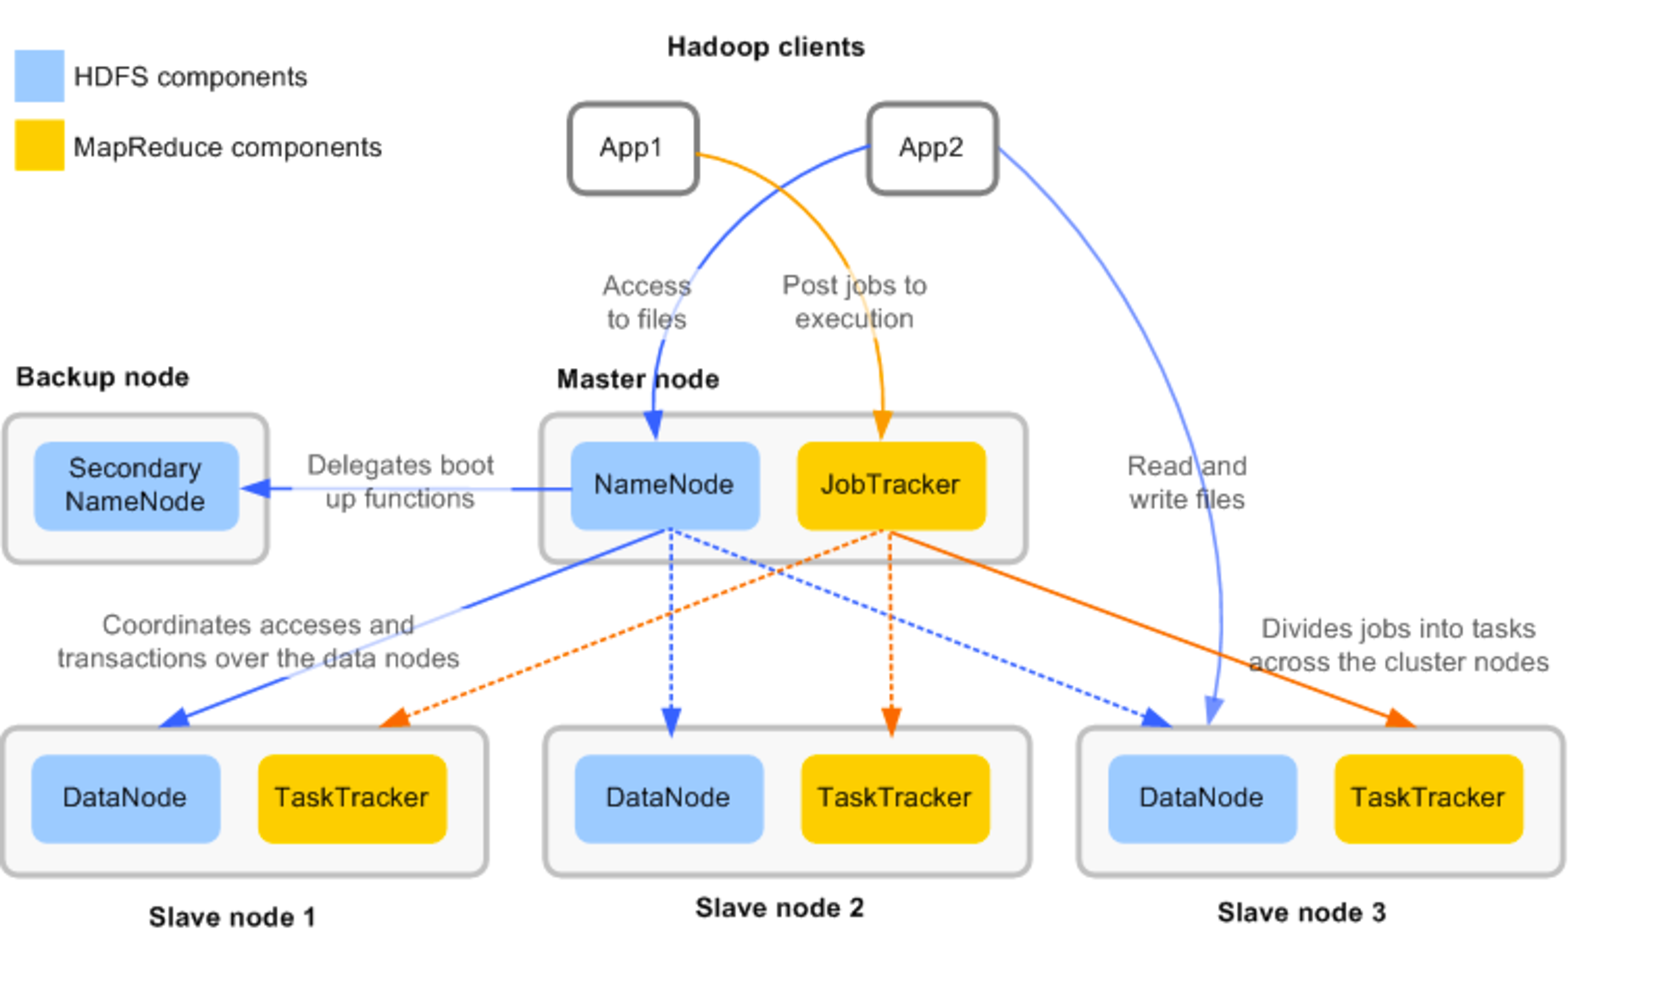
\includegraphics[width=5in]{hadooparch.pdf}
  \caption{Hadoop系统架构}
  \label{fig:hadooparch}
\end{figure}

在这个启动过程中,Hadoop集群中的每一台服务器都需要载入配置参数。这些配
置参数并未维护在一个集中的位置而是存储在每一台服务器上。用户通过手动的
同步操作将配置文件同步到集群的所有服务器上。在每一台服务器上,
\textit{NameNode/DataNode}会首先启动,在本地配置文件在进程空间里生成
一个Configuration对象,紧接着\textit{JobTracker/TaskTracker}启动,生成
JobConf对象。当用户编写一个在Hadoop上运行的MapReduce应用程序的时候,
都需要生成一个JobConf对象并且传递给\textit{JobTracker},此JobConf中的
配置会覆盖掉之前\textit{JobTracker}加载的JobConf对象;最后,当用户的任
务已经提交给\textit{JobTracker},那么集群中的\textit{TaskTracker}都会
通过信条协议向\textit{JobTracker}请求最新的可执行的任务,当获得任务后
将根据其种类(Map任务或Reduce任务)来启动对应的任务,启动的过程中会生成
一个JobConf对象,该对象加载\textit{TaskTracker}本地的配置文件以及用户
提交的JobConf中的数据。

事实上,动态的对于那些已经加载到Hadoop运行时系统中的参数进行修改非常困难。比如参数
\textit{mapred.job.tracker.handler.count}值会决定\textit{JobTracker}中
启动的服务线程的数目。而这些服务线程是在\textit{JobTracker}启动的时候开辟的
线程池。因此即便我们在运行时修改了这个参数,也不会对当前运行中的系统行为产生任何影
响。本文中,对Hadoop集群参数的修改是通过将新生成的参数写入到本地配置文件中,
在下一次启动的时候让Hadoop自动加载实现的。

\section{基于模糊逻辑的配置算法}

\subsection{运行时数据搜集}
我们通过修改Hadoop源码以及分布式的资源检测工具来获得集群的历史运行数据
和所有服务器的硬件指标。并且使用这些信息作为模糊逻辑方案的输入数据来来
计算参数。

\begin{enumerate}
\item 所有节点的Map运行时间的平均值和本节点Map任务执行时间的差
\item 所有节点的Reduce运行平均时间和本节点上Reduce任务执行平均时间差
\item 服务器在执行任务过程中的CPU平均负载
\end{enumerate}

同时我们也需要集群中服务器的硬件指标,包括:
\begin{enumerate}
\item 服务器的CPU频率,以及核心数目。
\item 服务器的内存容量
\item 服务器的硬盘参数
\item 服务器的网络带宽以及接入机架信息
\end{enumerate}
    
\subsection{模糊控制器的实现}
\subsubsection{隶属度函数}
我们使用了混合的隶属度函数来描述Hadoop集群的各种硬件信息,其中包括高斯
型隶属度函数、梯形隶属度函数。梯形隶属度函数能够更好的体现离散输入的特
点,比较适合Hadoop集群中服务器硬件指标数据。

三个隶属度函数分别为:
\begin{equation}
  \label{equa:likelyhoods}
  \begin{split}
    y_{Slow} = gaussmf(x, [sig, c])[sig=2, c=0]\\
    y_{Average} = trapmf(x, [a, b, c, d])[a=3, b=4.5, c=5.5., d=6.2]\\
    y_{Flat} = smf(x, [a, b])[a=4.5, b=9]
  \end{split}
\end{equation}
其中高斯和梯形隶属度函数的表达式如下:
\begin{equation}
  \label{equal:two}
  \begin{split}
    f(x;\sigma,c) = e^{\frac{(x-c)^2}{2\sigma^2}}\\
    f(x;a,b,c,d)=max(min(\frac{x-a}{b-a},1,\frac{d-x}{d-c}),0)
  \end{split}
\end{equation}

实际使用中,服务器CPU频率的变化范围设定为[0,16GHz]。当前主流的CPU为4核,
单核频率2GHz,因此8GHz作为中间值,超过16GHz的单服务器计算能力称为
\textit{很快}的CPU。模糊子集分别为\textit{Slow, Average, Fast},其隶属
度函数在Matlab中可以表示为图\ref{fig:cpulikelyhood}所示。单机CPU频率无
上限,因此使用S型隶属度函数来描述\textit{Fast}。

\begin{figure}[h!]
  \centering
  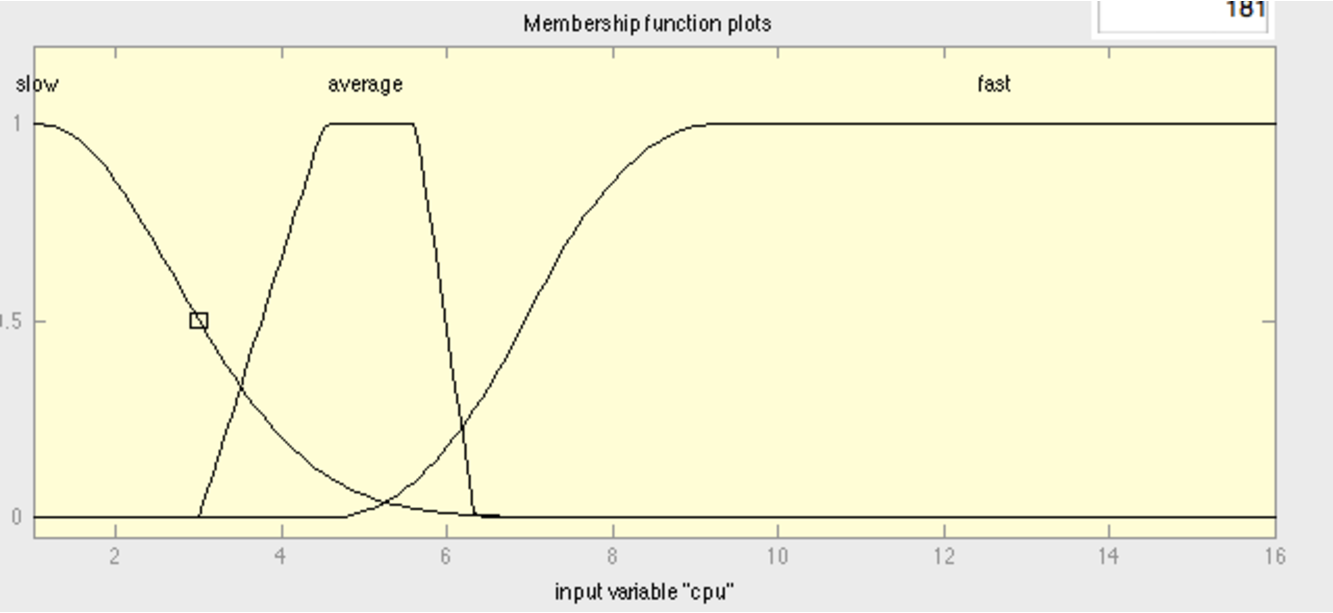
\includegraphics[width=5in]{cpulikely.pdf}
  \caption{对CPU建模的隶属度函数分布图}
  \label{fig:cpulikelyhood}
\end{figure}

分别对内存,网络进行建模,生成如下隶属度函数图
(\ref{fig:memlikelyhood}和\ref{fig:networklikelyhood})

\begin{figure}[h!]
  \centering
  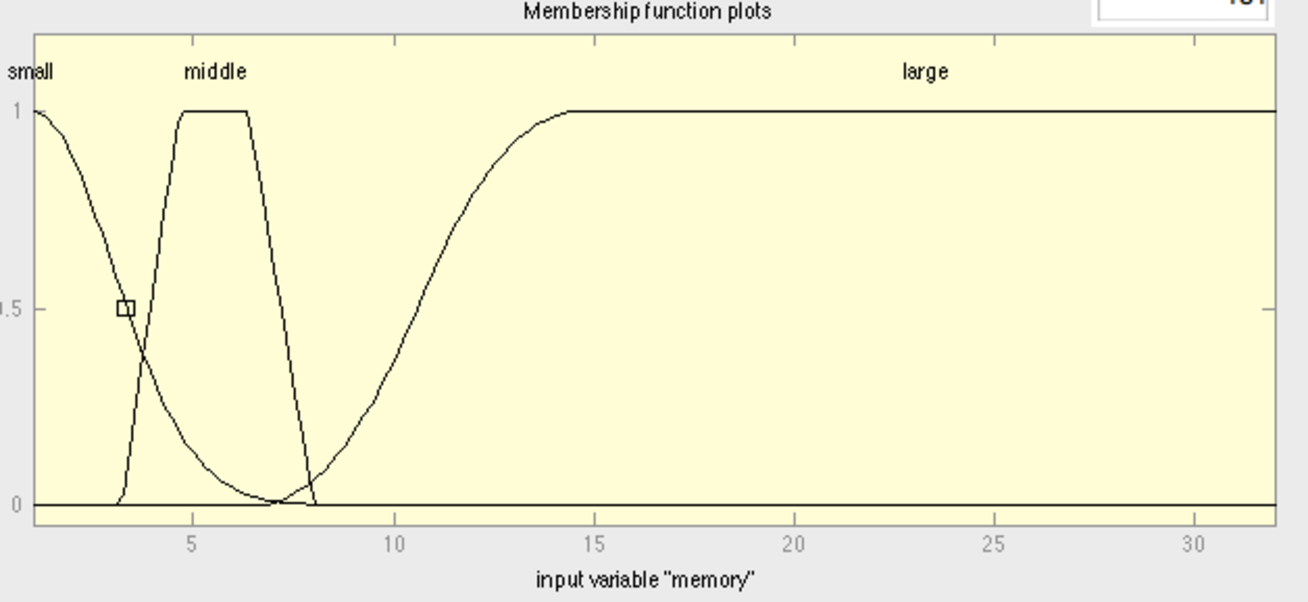
\includegraphics[width=5in]{memlikely.pdf}
  \caption{对内存建模的隶属度函数分布图}
  \label{fig:memlikelyhood}
\end{figure}

\begin{figure}[h!]
  \centering
  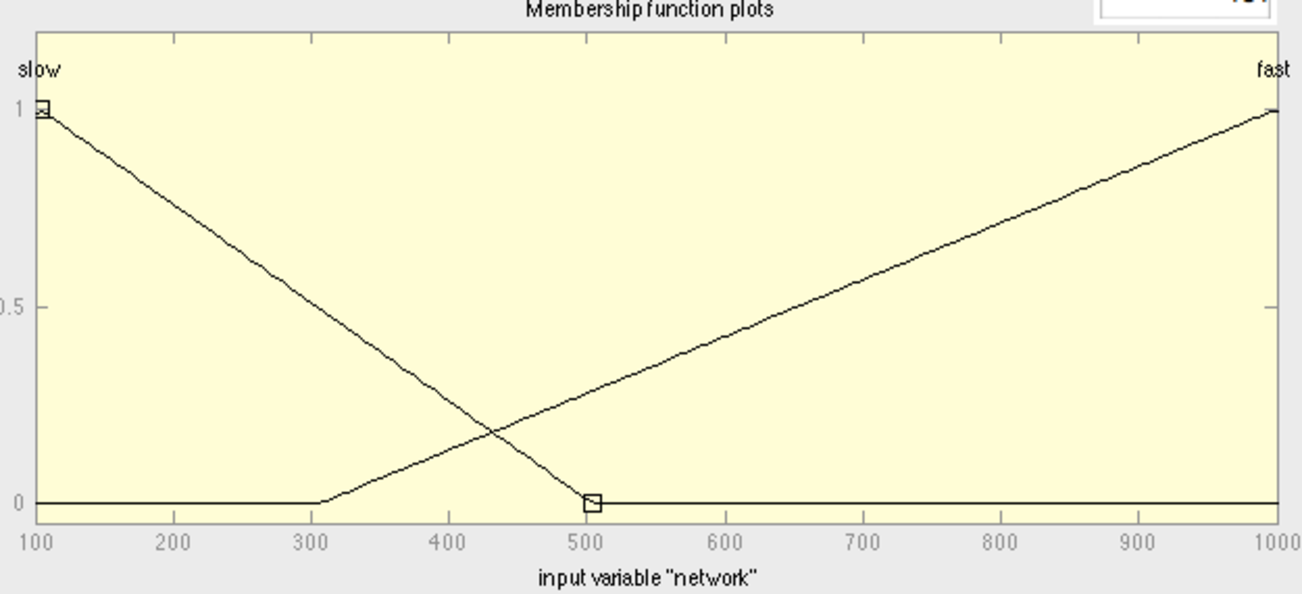
\includegraphics[width=5in]{networklikely.pdf}
  \caption{对网络建模的隶属度函数分布图}
  \label{fig:networklikelyhood}
\end{figure}

另一个输入来源就是执行的历史信息。在本文中我们认为任务执行的历史信息是
由多种原因造成的,特别是临时的错误,调度器的优先级等。因此它们并不适合
作为参数直接来影响模糊推理的结果,我们用它们作为最后的微调参数。

模糊逻辑的输出值为Hadoop配置参数中的值,我们在这里考虑了10个对系统性能
影响较大的参数\cite{hadoopconfexample, hadooptuning, speeduphadoop}.

\begin{table}[h!]\small
  \caption{模糊逻辑输出参数列表}
  \label{table:outputvars}
  \centering
  \begin{tabular}{|l c|}
    \hline
    \textit{参数名称} & \textit{取值范围} \\
    \hline
    io.sort.mb & 10-48-96-192-384-768 M \\
    \hline
    io.sort.factor & 10-40-80-120-240\\
    \hline
    io.sort.split.percent & 0-0.2-0.4-0.6-0.8-1.0\\
    \hline
    mapred.reduce.parallel.copies & 1-5-10-15-20\\
    \hline
    mapred.min.split.size & 64-128-256-512 M\\
    \hline
    mapred.tasktracker.reduce/map & \\
    .task.maximum & 1(1)-2(3)-3(5)-4(6)-5(9)\\
    \hline
    dfs.block.size & 64-128-256-512 M\\
    \hline
    mapred.map.tasks.speculative.execution & False -> True \\
    \hline
    mapred.reduce.task.speculative.execution & False -> True\\
    \hline
    mapred.job.shuffle.merge.percent & 0-0.2-0.4-0.6-0.8-1.0\\
    \hline
    mapred.job.shuffle.input.buffer.percent & 0-0.2-0.4-0.6-0.8-1.0\\
    \hline
  \end{tabular}
\end{table}

\subsubsection{模糊推理规则}
通过系统的调研Hadoop邮件列表中关于优化配置的参数和场景,我们为模糊算法
设定了合理的模糊规则。由于输入变量数目较多,输出变量更多,我们仅仅列出
其中一个模糊规则作为示例。\textit{io.sort.mb}指Hadoop的MapReduce任务执行过程中
对键值对进行排序时候可以使用的内存buffer的容量,单位为MB。
\textit{io.sort.mb}的隶属度集合如图\ref{fig:iomblikely}所示。

\begin{figure}[h!]
  \centering
  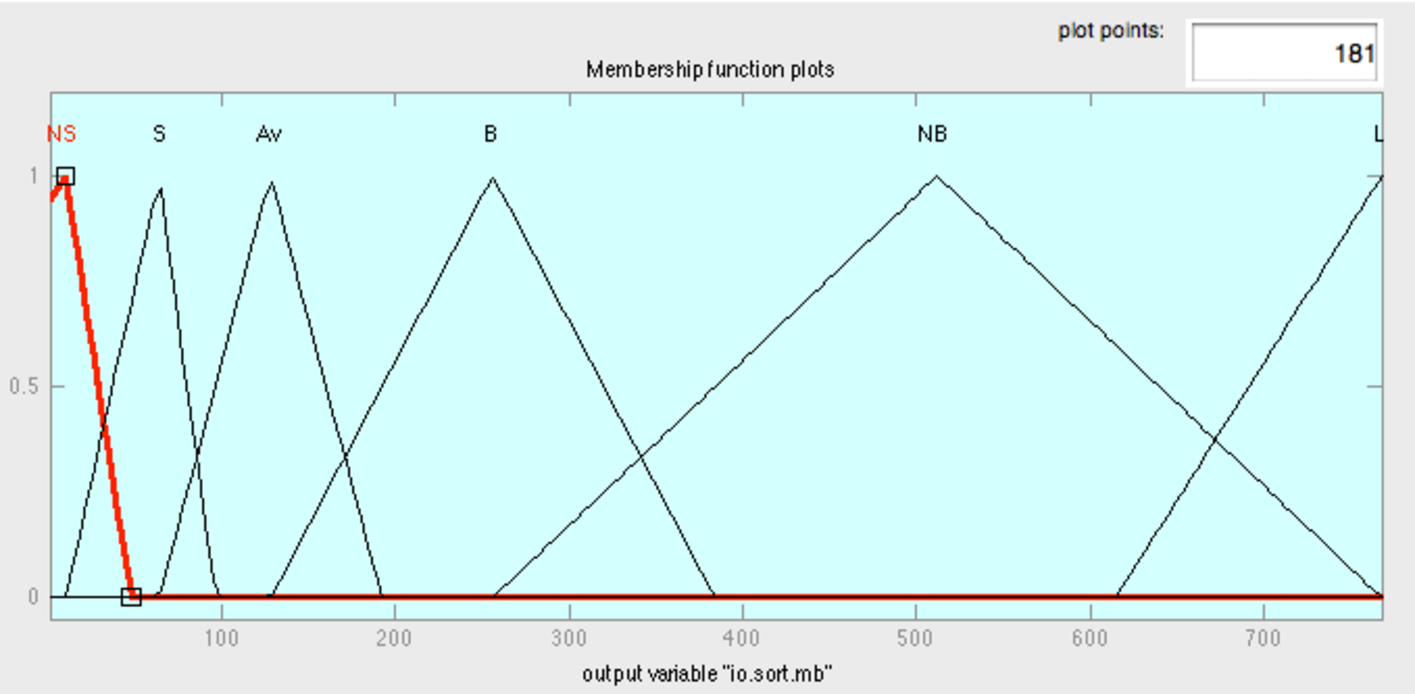
\includegraphics[width=5in]{iomblikeley.pdf}
  \caption{\textit{io.sort.mb}的隶属度函数}
  \label{fig:iomblikely}
\end{figure}

其对应的规则如图\ref{fig:iombrule}所示。

\begin{figure}[h!]
  \centering
  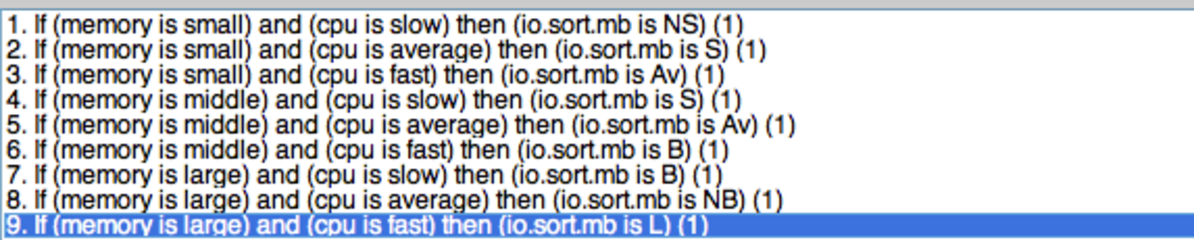
\includegraphics[width=5in]{iombrule.pdf}
  \caption{对\textit{io.sort.mb}的模糊规则表}
  \label{fig:iombrule}
\end{figure}

\section{实验和分析}
\subsection{Matlab仿真}
利用Matlab实现的模糊控制系统架构图(FIS)如下图\ref{fig:fis}所示。
\begin{figure}[h!]
  \centering
  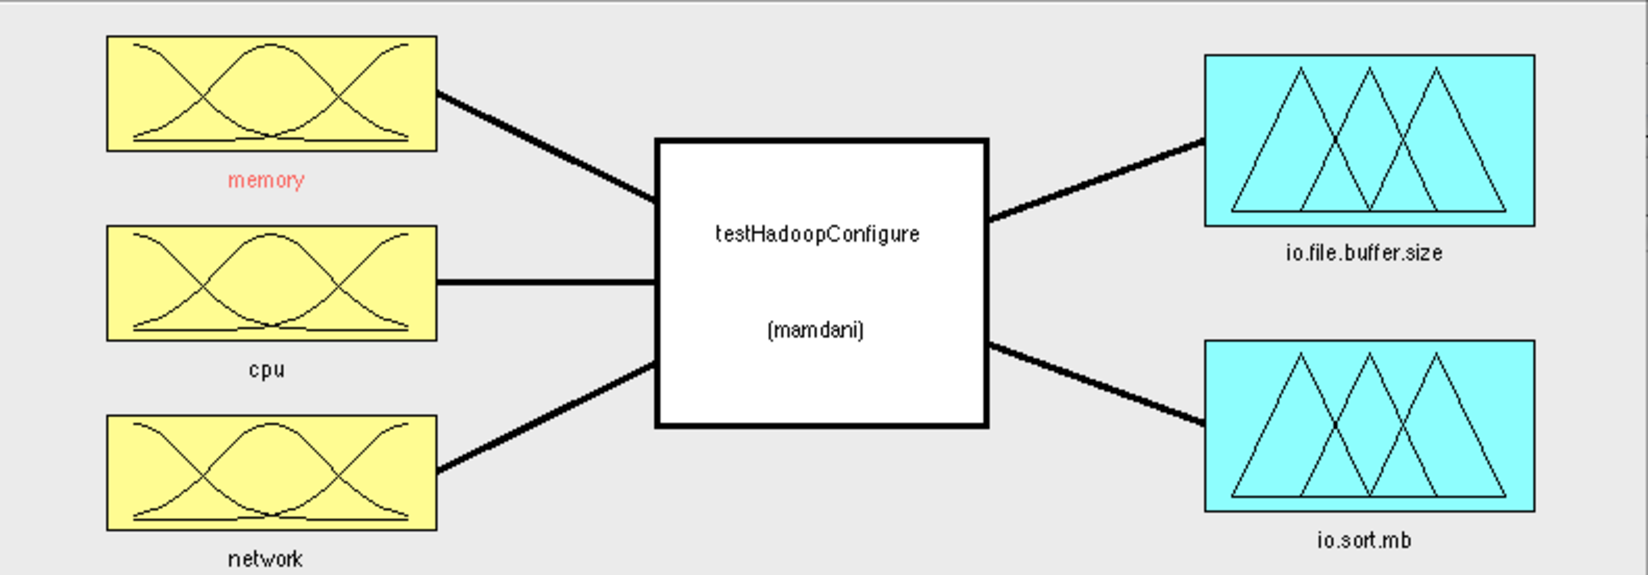
\includegraphics[width=5in]{fuzzyfis.pdf}
  \caption{系统的模糊控制系统总体图(仅列出了三个输入参数和两个输出参数)}
  \label{fig:fis}
\end{figure}
利用sufview可以得到\textit{io.sort.mb}和服务器中内存、CPU参数的输出曲
面,图\ref{fig:matlab}所示。
\begin{figure}[h!]
  \centering
  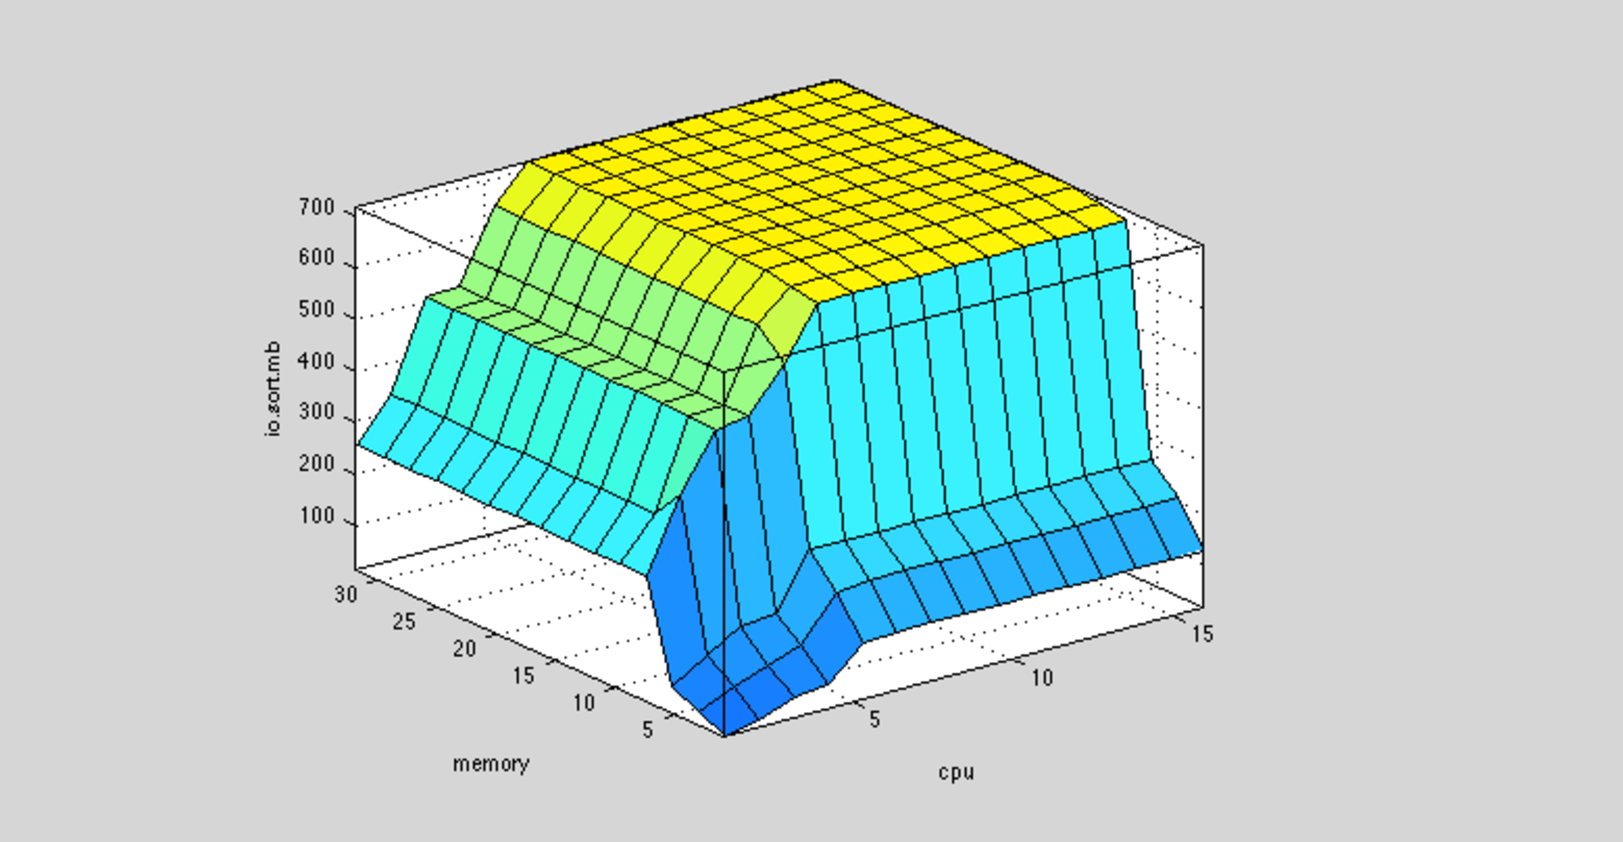
\includegraphics[width=5in]{matlab.pdf}
  \caption{参数\textit{io.sort.mb}的模糊规则输出三维示意图}
  \label{fig:matlab}
\end{figure}

\subsection{Hadoop集群实验}
通过修改Hadoop的源代码,我们为\textit{JobTracker}和
\textit{TaskTracker}实现了自动配置代码,通过检查历史运行数据来判断是否
需要重新配置,并将根据模糊逻辑生成的参数写入到本地配置文件中。

\subsubsection{同构环境实验}

所有的实验在一个由4台服务器构成的Hadoop集群上进行,其中3台slave节点,
一台master节点,所有节点性能配置如表\ref{table:machines}所示。

\begin{table}[h!]\small
  \caption{同构集群的节点参数}
  \label{table:machines}
  \centering
  \begin{tabular}{|c|c|}
    \hline
    \textit{属性} & \textit{参数} \\
    \hline
    CPU & Xeon W3530 2.53GHz\\
    \hline
    Memory & 6G 1066MHz ECC\\
    \hline
    Disk & 1T SATA Raid 1\\
    \hline
    Network & 100MB Ethernet\\
    \hline
  \end{tabular}
\end{table}

实验基于Hadoop发行版中自带的Terasort应用。使用默认配置参数运行该引用之后,再次使用自动化配置后得到的参数
运行Terasort,多次实验(每个实验执行10次)平均后比较性能。输入数据为25GB,最后结果如表\ref{table:tera1}所示。

\begin{table}[h!]\small
  \caption{运行25G Terasort所花费的时间}
  \label{table:tera1}
  \centering
  \begin{tabular}{|c|c|c|}
    \hline
    & \textit{Default} & \textit{Autoconfigured}\\
    \hline
    & 44min & 19min,40s\\
    Tera-Sort & &\\
    & 376maps, 16min & 94maps, 1min\\
    & 1reduce, 43min & 3reduce, 19min\\
    \hline
  \end{tabular}
\end{table}

采用默认配置的Hadoop集群运行一次任务需要2640s,
其中共运行了376个map任务共耗时960s,一个reduce任务,耗时2580秒。采用我
们的模糊推理得到的参数运行同一个任务只需要1180s,其中公允性了94个map任
务耗时60秒,3个reduce任务,耗时1140秒,加速比为2.23.此实验结果表明使用
模糊逻辑配置的工具能够得到较好的集群性能。


\subsubsection{异构环境实验}
通过人为降低集群中某一台服务器的内存,并且使其只启动一个CPU核来构
造异构的环境,该服务器的配置如下表\ref{table:m2}所示。

\begin{table}[h!]\small
  \caption{同构集群的节点参数}
  \label{table:m2}
  \centering
  \begin{tabular}{|c|c|}
    \hline
    \textit{属性} & \textit{参数} \\
    \hline
    CPU &  OneCore  2.53GHz\\
    \hline
    Memory & 2G 1066MHz ECC\\
    \hline
    Disk & 1T SATA Raid 1\\
    \hline
    Network & 100MB Ethernet\\
    \hline
  \end{tabular}
\end{table}

同样使用Terasort作为基准测试,并且和之前同构环境下测试时生成的
配置文件进行比较。执行10次后平均时间如表\ref{table:tera2}所示。

\begin{table}[h!]\small
  \caption{运行25G Terasort 同构和异构配置的性能对比}
  \label{table:tera2}
  \centering
  \begin{tabular}{|c|c|c|}
    \hline
    & \textit{homo-configured} & \textit{heter-configured}\\
    \hline
    & 33min & 27min\\
    Tera-Sort & &\\
    & 94maps, 11min & 94maps, 7min\\
    & 3reduce, 31min & 3reduces, 25min\\
    \hline
  \end{tabular}
\end{table}

结合表\ref{table:tera1}和\ref{table:tera2},我们可以得出结论,采用同构
环境下计算出来的结果来配置异构集群会使得集群性能降低,并且这个性能降低
(从19min到33min)远远超过了一台服务器性能折半带来的性能降低。这说明了在
异构环境下使用正确的参数配置的重要性。通过实验结果也可以看出来,采用异
构配置的集群其性能明显优于同构的配置参数。

\section{小结}
本研究使用模糊逻辑的方法对大规模部署的异构Hadoop集群进行参数
配置,并且通过试验证明了本方法能够明显的提高Hadoop集群中MapReduce任务
执行的速度。然而面临着不断出现的对系统反应时间有着更高要求的应用,
Hadoop和MapReduce模型本身的设计上的限制决定了其无法适用于这类应用。从
下一章开始,我们将介绍新型的分布式存储系统以及新的计算模型来进一步应对
实时应用的需求。

  \chapter{基于内存的分布式键值存储系统}
\label{chapter:sedna}

\section{引言}
云计算平台上的存储系统和传统的网络存储系统不同,它不仅仅要对外服务接受来自客户端的读写请求,更重要的是为云计算平台中运行的分布式任务提供并发的数据读写能力。图\ref{fig:app}展示了一个典型的云计算环境下,数据中心内部存储的架构图:存储通过大量的廉价个人计算机构成,存储系统不仅仅接受来自外界的读写请求,更需要支撑数据中心内部运行的应用程序的读写请求。

\begin{figure}[h!]
\centering
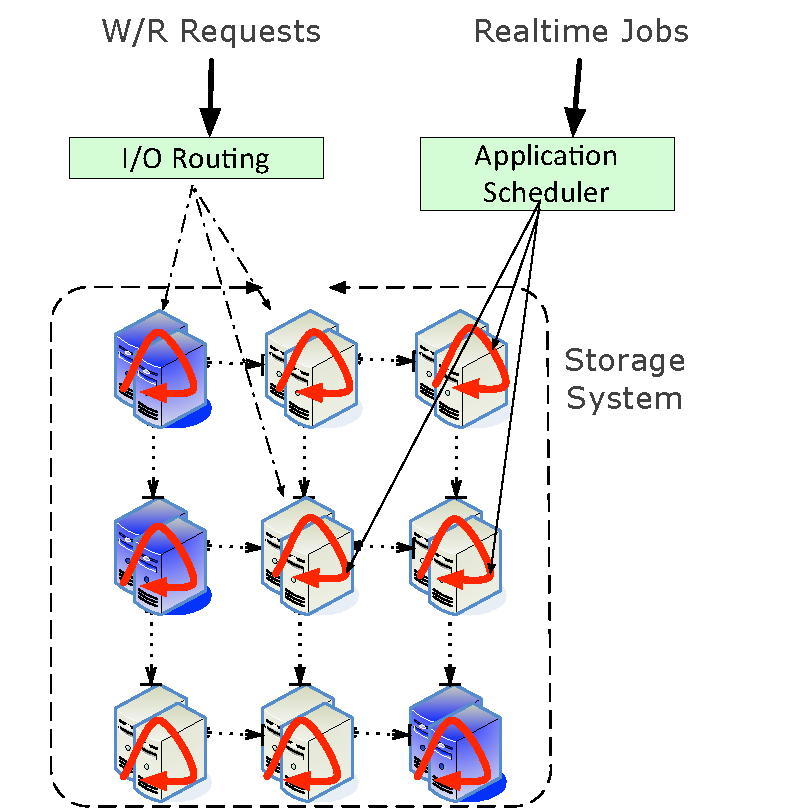
\includegraphics[height=3in, width=3.5in]{../figures/app.pdf}
\caption{典型的云计算环境下数据中心中存储架构图}
\label{fig:app}
\end{figure}

为了存储各种不同类型的数据并支撑不同类型的应用程序,云计算领域出现了多种分布式存储系统。早期以Google File System\cite{Ghemawat2003}为代表的块式存储多用来存储只会被追加写的较大的文件,因此适合连续的对数据块进行读取。这类存储系统最早出现在搜索引擎相关的系统中,主要是由于通用搜索引擎对廉价集群上进行海量数据存储的需求。后来以Dynamo\cite{decandia2007dynamo}为代表的分布式的键值存储系统开始出现。这类存储系统专用于存储较小的数据且支持对这些数据进行随机读写。在键值存储系统的基础上,出现了被称为NoSQL\cite{nosqldatabase}的海量结构化存储系统,如Bigtable\cite{chang2008bigtable}、Cassandra\cite{lakshman2010cassandra}等,这类存储系统多用来存储具有结构化信息的数据,数据按\textit{表}组织,表中每一个单元存储的数据都较小并且支持随机的读写。

这些存储系统虽然在存储的数据类型以及所支撑的应用类型上有区别,但它们都是基于硬盘(Hard Driver)构建的持久分布式存储系统。在对读写性能要求苛刻的场景下,它们的性能是不能接受的。比如Facebook网站的后台数据中心每秒需要承担10亿次随机读\cite{nishtala2013scaling},在这样的负载要求下,数据中心内部需要部署像Redis\cite{redis},Memcached\cite{memcachedproject}这样的分布式内存缓存来提高读写速率。分布式缓存系统通过在内存中构建非持久的哈希表为应用提供高速随机访问能力。不过作为缓存系统,其不能脱离一个持久存储系统独立存在,更无法保证数据的持久性。2009年提出的RamCloud\cite{ousterhout2010case}在完全基于内存的基础上为数据提供了持久性保障以及快速数据恢复能力,可以作为独立的高速分布式存储系统使用。

从分布式存储的发展路径可以看出,随着社交网络,电子商务,在线广告系统的发展,小的、零散的原始数据现在已经成为应用程序最主要的数据来源,云计算环境下的存储系统也在向高速读写、随机访问、海量小数据的方向发展。在本章中,我们将介绍另一个完全基于内存实现的持久化的分布式键值存储系统——Sedna。该系统通过引入新的集群架构、节点管理算法、以及新的API进一步提高了海量内存存储系统的存储容量、随机访问速度、数据一致性等方面的性能,并通过为用户提供了一个简单、有效的实时API来支持各类实时应用。\ref{section:relevant}节介绍现有存储系统上的相关工作,以及内存存储的合理性和主要挑战。\ref{section:techs}节详细描述Sedna的架构和实现细节,\ref{section:exp3}节通过实验着重分析了Sedna的读写性能,\ref{section:con3}节对本章进行了小结。

\section{相关工作简介}
\label{section:relevant}

\subsection{相关分布式存储系统介绍}
Google File System由Google公司与2003年提出的使用海量廉价个人计算机实现的基于块的大规模分布式文件系统,其基本架构如图\ref{fig:gfsarch}所示,包括一个master和多个chunkserver组成。文件系统的层次结构和名字空间都存放在GFS Master节点中,客户端应用程序首先通过查询GFS master来获得欲访问的文件所在节点信息(chunk location),然后通过向特定的节点发送读写请求来完成数据传输过程。

\begin{figure}[h!]
\centering
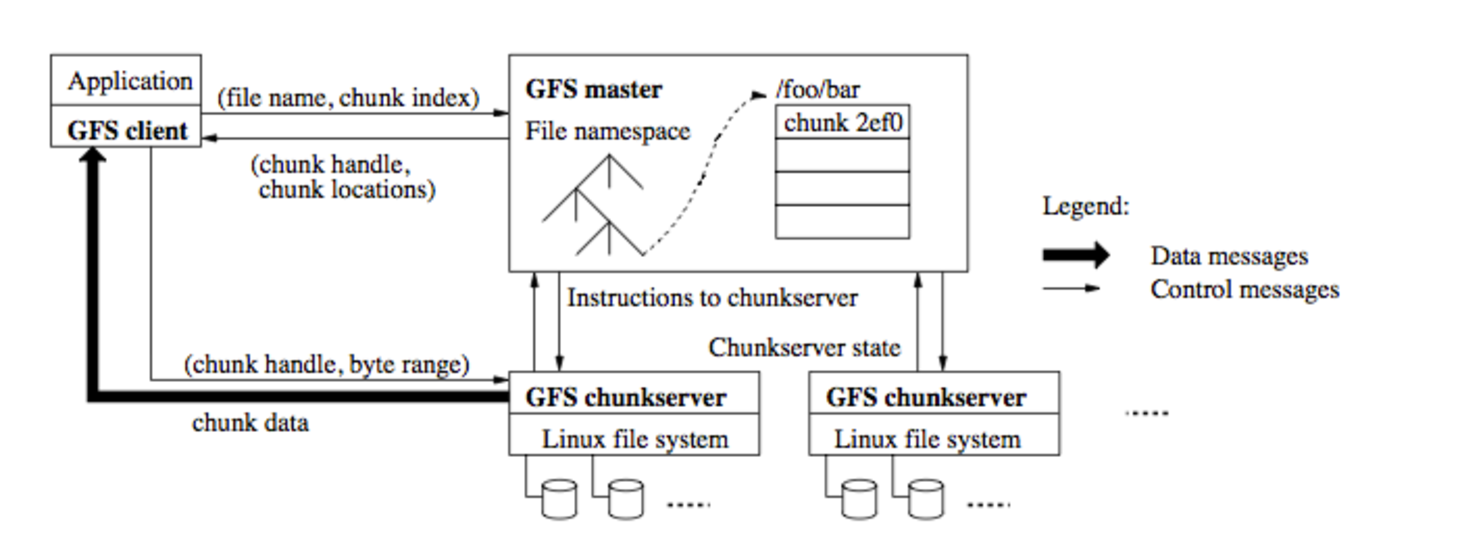
\includegraphics[width=6in]{../figures/gfsarch.pdf}
\caption{GFS文件系统的架构}
\label{fig:gfsarch}
\end{figure}

Hadoop Distributed File System(HDFS)是Apach基金会基于GFS实现的一套开源分布式存储系统。如图\ref{fig:hdfsarch}所示,HDFS中NameNode和DataNode分别对应了GFS中的Master和Chunkserver。类似GFS,任何一个文件都由预定义大小(默认64MB)的块组成,这些块被冗余存储于多个DataNode上(默认情况下,每一个块会存储在三个节点中)。由于HDFS运行在由海量个人计算机构成的数据中心中,节点失效和网络故障比较常见,通过多备份实现了系统的可用性和容错性。每一个DataNode需要和NameNode维持一个周期心跳用来检测节点是否失效以及网络是否可用,当NameNode发现某节点失效的时候会利用备份节点的数据来提供服务,并且尝试恢复失效节点,以维持每一个数据块多备份的状态。由于每一个客户端在访问HDFS中的数据时都需要向NameNode查询相关数据所在的DataNode位置信息,为了保证多个客户端程序读写的性能,HDFS的实现中会将所有的命名空间信息都存放在NameNode的内存中。

\begin{figure}[h!]
	\centering
	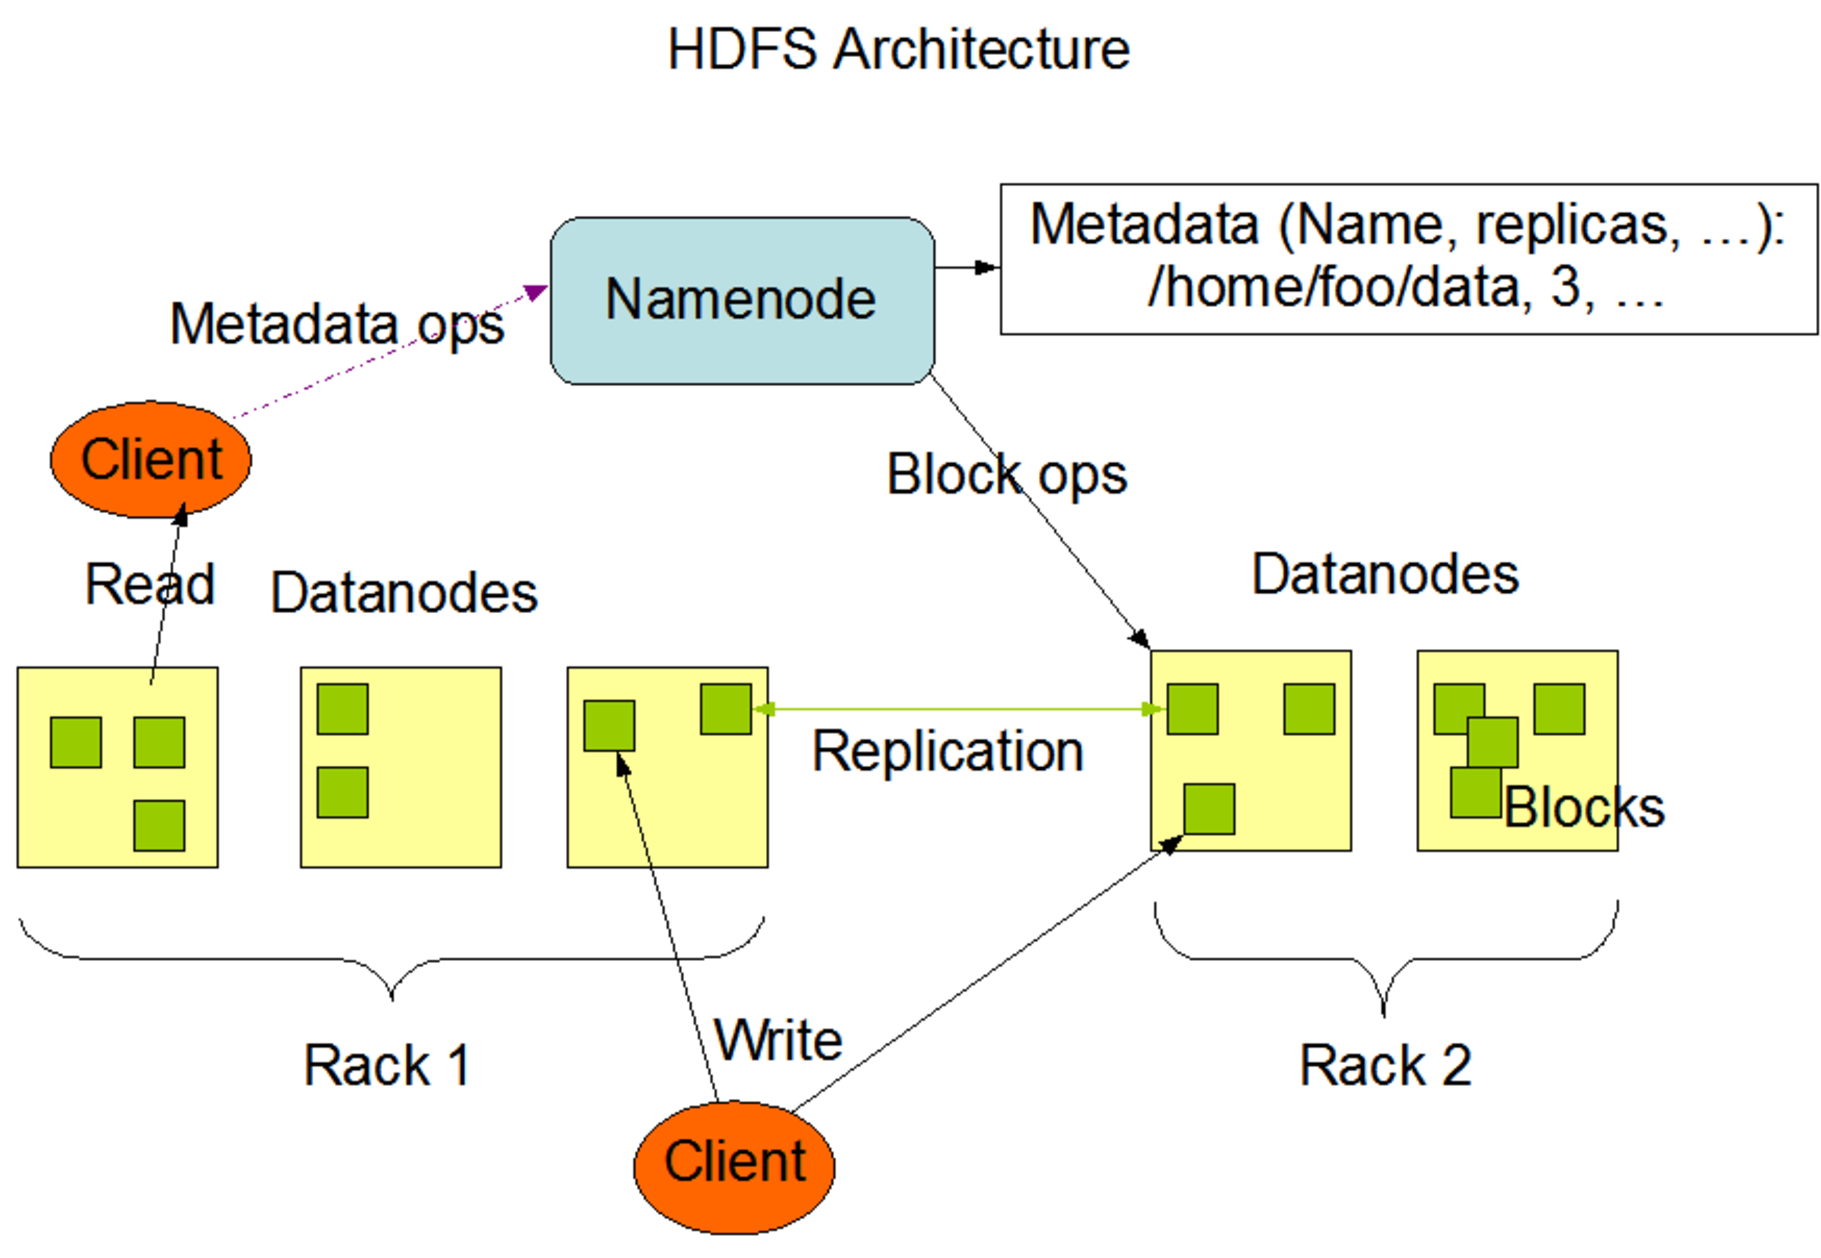
\includegraphics[width=5in]{hdfsarchitecture.pdf}
	\caption{HDFS文件系统架构图}
	\label{fig:hdfsarch}
\end{figure}

HDFS这种以数据块为基本单元的方法提高了系统对于海量文件的存储能力。通过单个NameNode可以管理成千上万服务器构成的存储集群。但是这种方案同时也带来了一些很明显的问题,其中两个比较典型的是:NameNode的单点故障和集群存储容量受限于单台服务器性能。

对于单点故障问题,2011年Borthakur\cite{borthakur2011apache}提出了使用AvatarNode代替NameNode和SecondaryNameNode的方案,系统架构如图(\ref{fig:avatar})所示:HDFS集群包含两个avatar节点,active avatar和standby avatar。任一个avatar节点实际上都是一个正常的NameNode的包裹。HDFS文件系统镜像和日志都存放在NFS中,而不是本地。活动的avatar节点将所有的事务写入在NFS中的log文件中,与此同时,standby avatar节点将从NFS中打开相同的log文件,读入并且不断的将新写入的事务应用到本地存储的命名空间中,从而使得本地的命名空间和当前活跃avatar节点上的命名空间保持尽量一致。所有的DataNode不仅仅和active avatar节点交流还会和standby avatar节点交流,这样就使得standby的avatar节点时刻保持着最新的块位置信息。在active avatar失效的时候,standby avatar节点能够在一分钟内开始提供服务。

\begin{figure}[h!]
\centering
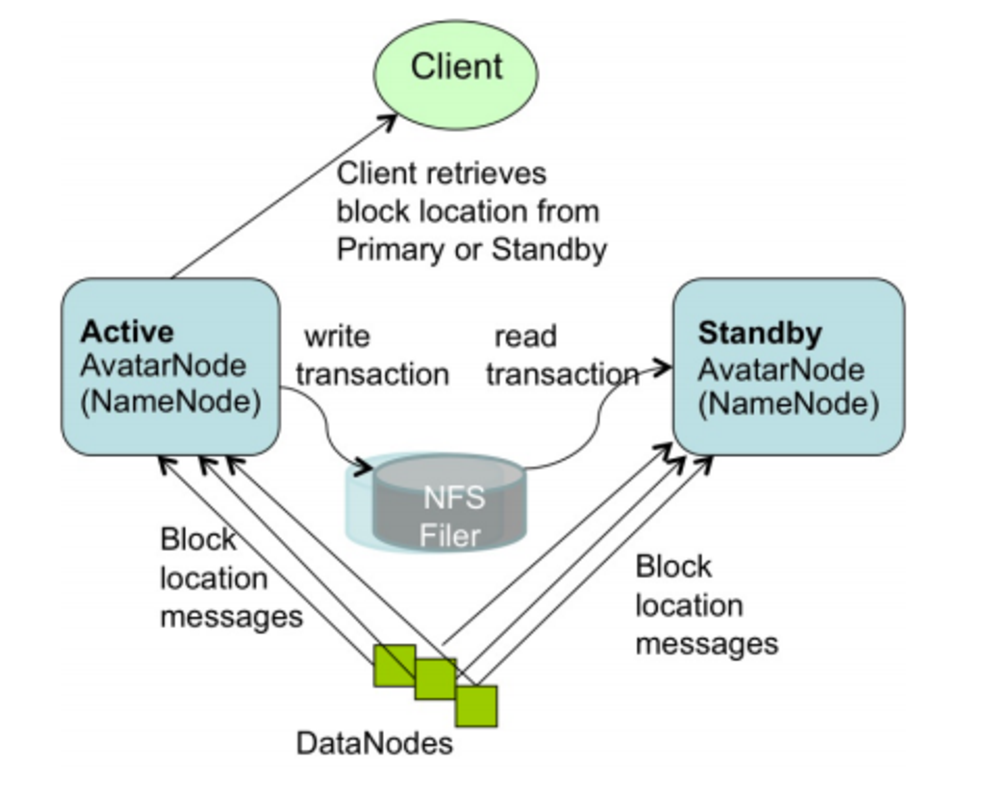
\includegraphics[height=3.5in]{../figures/avatarfb.pdf}
\caption{Avatar Node架构}
\label{fig:avatar}
\end{figure}

容量瓶颈问题同样严重,Konstantin V. Shavachko的论文\cite{shvachko2011apache}详细探讨了HDFS文件系统的瓶颈。通过对当时最大的HDFS集群的实际运行数据的搜集和分析,得到了单个NameNode服务器上内存容量和整个HDFS集群存储容量上限的关系:假设每一个块的位置信息都需要在NameNode中占据超过200个字节的内存,而在一个文件平均包括1.5个块的集群中,每一个文件就大概需要600个字节的内存空间。这样,如果要存储超过1亿个文件,那么NameNode至少就要有60GB的内存。如果该HDFS集群中每一个块为128MB,并且备份三分,那么总的存储空间就是60PB(NameNode需要60GB内存),这也就意味着HDFS的架构不具备线性扩展性。论文\cite{mckusick2009gfs}提出了一种新的GFS Namespace 服务器的架构。这种新的架构包含了数以百计的Namespace服务器,每一个服务器上最多支持超过1亿个文件。由于NameNode容量的提高,每一个文件可以被划分为更加细粒度的块(由64MB可以减少到1MB),用以支持小数据存储。

由于块式存储系统在随机读写上性能较差,出现了多种针对小数据随机访问模式的键值存储系统。Dynamo\cite{decandia2007dynamo}是2006年Amazon公司提出的一种高可用的键值存储系统。从存储内容来说,Dynamo是一种存储键值对的存储系统;从应用场景来说,Dynamo主要应用于\textit{永远可写}的场景中。比如在Amazon网站的购物车应用中,用户任意一次的\textit{加入购物车}动作都应该成功,不管这次请求时数据中心内部是否发生了错误。从架构上来说,Dynamo彻底抛弃了GFS的单中心节点架构,提出了一套基于对等网络的P2P架构。所有的节点都等价的提供服务,节点和节点之间松耦合,单个节点失效不会影响到别的节点。为了提供高可用,高速随机写的能力,Dynamo整合了一系列分布式系统技术:采用动态哈希表和一致性哈希来进行数据划分和复制备份;使用多版本和矢量时钟技术来提供一致性;多副本之间的一致性由仲裁算法来保持一致性;采用反熵(anti-entropy based recovery)的恢复策略;采用基于gossip的分布式故障检测及token协议等。

Megastore\cite{baker2011megastore}是由Google于2011年公开的跨数据中心存储系统。它在保证扩放性的前提下,提供了传统RDBMS具备的易用性,包括强一致性保证、高可用性,并且在细粒度的数据分片中提供了ACID的语义。Megastore通过允许应用程序细粒度的管理数据分片和本地性,从而避免了CAP\cite{gilbert2002brewer}的限制。在Megastore中以EntityGroup作为基本的独立数据集合,一个EntityGroup中的数据并且会在不同的数据中心间同步复制。除此之外,Megastore还使用Paxos\cite{lamport2001paxos}协议避免了之前所提到的分布式主节点需要将写前日志(write-ahead-log)复制到多个节点的耗时操作。

\begin{figure}[h!]
\centering
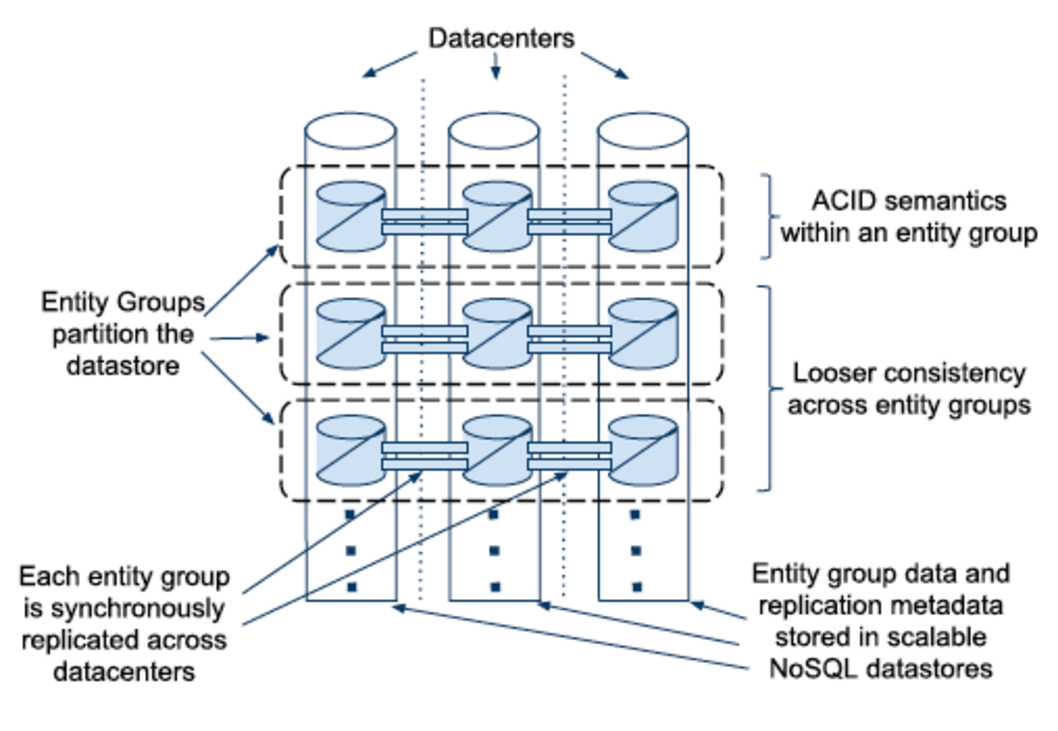
\includegraphics[width=4in]{../figures/megastore.pdf}
\caption{Megastore架构图}
\label{fig:megastore}
\end{figure}

图(\ref{fig:megastore})展示了EntityGroup的结构以及它们是如何在不同的数据中心之间进行复制的。在一个EntityGroup内部的所有操作都依赖于Paxos算法来确保其ACID的语义,而跨EntityGroup的操作则依赖于比较笨重的两阶段提交协议。在一个数据中心内部,Megastore使用Bigtable来做基础的容错存储。Megastore的创新点主要体现在下面几个方面:1)设计了EntityGroup方案给应用程序提供了足够的灵活性;2)使用Paxos算法来保证EntityGroup内部数据的强一致性。3)将分布式存储系统Bigtable和传统SQL模型相结合。

\subsection{内存存储的可行性和相关系统介绍}
实时应用在大规模数据处理应用中比重越来越大,得益于半导体技术的发展使得数
据产生的速度越来越高,数据存储的成本越来越低。实时应用对数据实时性的敏感度较高,
需要存储系统能够提供更高的读写速度。传统的基于磁盘的存储系统在随机读写上的局限性越来越明显。因此在实际应用中,多使用内存缓存系统在磁盘存储系统之上提供高速随机读写的能
力。比如世界上最大的社交网络Facebook,大量使用Memcached作内存缓存。以2009年8月的数据来看\cite{ousterhout2010case},大约其所有在线数据的25\%是保存在Memcached集群的内存中的,缓存提供了96.5\%的平均命中率。如果再算上数据库服务器的内存缓存,那么整个数据集(除去图片)大约有75\%的数据是存放在内存中的。从Facebook数据在内存缓存的比率来看,海量数据的场景下,使用内存来作为唯一的在线存储是可能的。

使用内存缓存系统似乎能够在较高的命中率的基础上以较少的内存代价(如在Facebook中,25\%的数据存储在内存中提供了96.5\%的命中率)来提供较高的平均访问时间。然而,由于磁盘和内存之间处理时间之间差超过1000倍,使得一次未命中会导致非常明显的访问延迟,这往往是不可以接受的。而且缓存机制带来的冷启动、数据抖动都埋下了性能急剧降低的隐患。

\begin{figure}[h!]
  \centering
  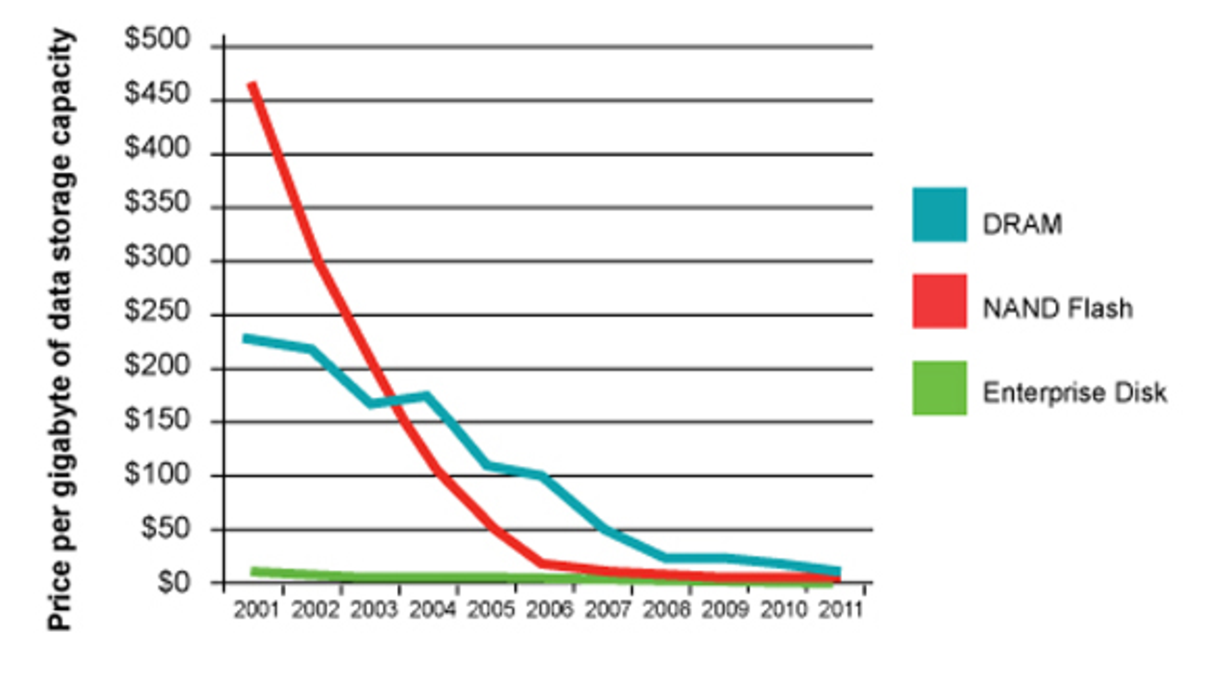
\includegraphics[width=3.5in]{../figures/mp.pdf}
  \caption{最近十年(2001-2011)内存,磁盘,Flash单位Gb的价格趋势分析。}
  \label{fig:price}
\end{figure}

因此在数据中心内部完全使用内存作为主要的存储介质,将硬盘(Hard Disk)作
为备份存储介质逐渐成为提高存储系统性能的主要手段。使用内存作为海量存
储的主要介质的可能性随着内存价格的逐步降低已经越来越大,图
\ref{fig:price}展示了十年来存储每Gb的数据,需要的成本对比图,从图中
我们可以看出来,随着半导体技术的发展,DRAM的成本有了一个极为明显的下降
过程,按照这个趋势,单位GB内存价格将持续走低,未来单机大规模内存会成为
主流。结合表\ref{table:price2}除去数据中心中网络和机架
成本,仅仅计算DRAM的成本,到2020年,我们可以通过假设4,000台服务器的集
群来提供超过1PB内存数据存储能力,而每GB的存储成本只有\$6。


\begin{table}[]\small
\caption{2012年完全使用内存构造海量存储的成本以及2020年的预估\cite{ousterhout2010case}}
\label{table:price2}
\centering
\begin{tabular}{|p{108pt}|c|c|}
\hline
\textbf{} & \textbf{2010} & \textbf{2020}\\
\hline
\textit{服务器数目}& 2,000 & 4,000\\
\hline
\textit{单服务器容量}  & 24GB & 256GB\\
\hline
\textit{总存储容量} & 48TB & 1PB\\
\hline
 \textit{总体成本} & \$3.1M & \$6M \\
 \hline
\textit{每GB成本} & \$65 & \$6 \\
\hline
\textit{每秒操作数} & 2*$10^9$ & 4*$10^9$\\
\hline
\end{tabular}
\end{table}

图\ref{fig:ramcloud}展示了基于内存的RamCloud机群的结构。一个RamCloud实例包括大量存储服务器,每一台存储服务器包含两个部分:1)主(Master)服务负责在内存中管理RAMCloud对象,并且负责处理客户端的请求;2)备份(Backup)服务存储了来自主节点的备份数据,并且将其存放到磁盘和Flash中。每一个RAMCloud实例同时包括一个协作者(Coordinator)服务器,负责管理配置信息,比如存储服务器的网络地址,以及存储对象的位置信息。协作者将对象放置到不同的存储服务器。RamCloud是一个键值存储系统,数据按照键来分布到不同的服务器存储。一个连续的键值组织成一个表,数据量较小的表会存放在一个存储节点中,较大的表会被分割并且存储与多个节点。客户端程序不会控制表的配置,协作者负责存储表和存储服务器之间的映射信息,RAMCloud客户端库将会保存一些缓存信息以减少对协作者的访问。

\begin{figure}[htbp]
	\centering
	\subfloat[RamCloud架构图]{
		\label{fig:ramcloud}
		\begin{minipage}[t]{0.5\textwidth}
			\centering
			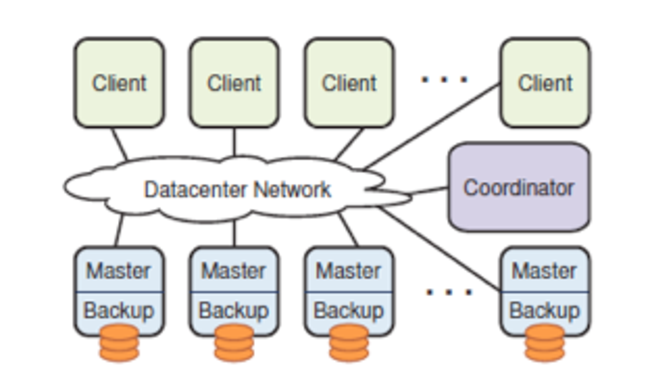
\includegraphics[width=2.8in]{ramcloud.pdf}
		\end{minipage}
	}
	\subfloat[RamCloud Log访问的结构图]{
		\label{fig:ramcloudlog}
		\begin{minipage}[t]{0.5\textwidth}
			\centering
			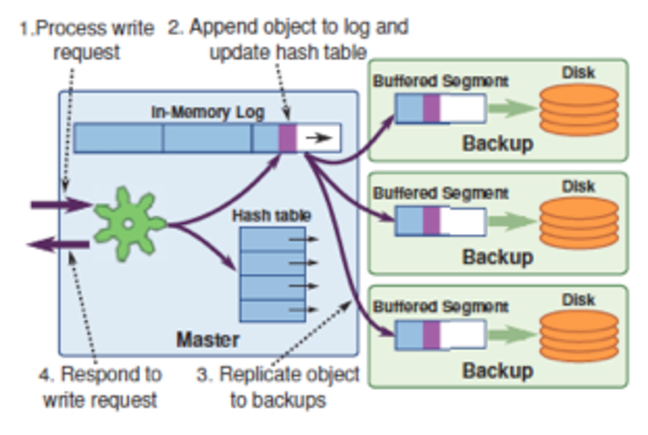
\includegraphics[width=2.8in]{ramcloudlog.pdf}
		\end{minipage}
	}
	\caption{RamCloud系统图示}
\end{figure}

RamCloud通过写备份的方式来保证数据的持久性\cite{ongaro2011fast},如图\ref{fig:ramcloudlog}所示,当一个存储节点中的主服务收到一个写请求的时候,它将首先更新自己内存中的哈希表,并将新的数据转发到多个备份节点中。备份节点将数据缓存在它们的内存中,最终写入本地磁盘。备份节点必须使用备份电源来确保即便在断电时,缓存中的数据也能被写入到本地磁盘中。基于内存在随机访问上的优势,RAMCloud能够极大的降低系统的访问延时,提高吞吐量,非常适应实时应用对存储系统的要求。

\subsection{前人工作的不足}
磁盘作为持久存储介质能够保证服务器在断电或重启后数据不会丢失,内存作为易失性介质,在掉电后所有的数据都会消失。因此基于内存的存储系统第一要解决的问题就是如何持久存储数据。这个问题上,RamCloud提出了一个有效的策略,它将内存中的数据备份到别的节点的内存和磁盘中,并且设计了一套快速恢复的策略,使得数据丢失后能够在几秒的时间内完全恢复。除了数据的持久性问题之外,我们认为还存在几个重要的基础性问题需要解决:
\begin{enumerate}
  \item 扩放性问题。由于单机内存的存储容量远远小于磁盘,内存集群若
    要达到和磁盘集群同样的存储能力需要更多服务器。因此,分布式内存存储
    系统需要具有更好的扩放性。单点故障和单点存储容量瓶颈都是不可以接受的。
    
  \item 读写效率问题。之所以使用内存作为存储介质是希望获得更好的数据
    访问效率从而满足实时应用的需求。传统的数据访问接口对于实时数据改
    变不够敏感,因此我们需要一个对数据改变响应更快的数据访问能力。
\end{enumerate}

\section{基于内存的分布式键值存储系统}
\label{section:techs}
面向实时应用的分布式存储系统应当具备的特点:
\begin{enumerate}
  \item 能够存储海量的小数据。小的、零散的原始数据现在已经成为云计
    算下应用程序最主要的数据来源。比如Twitter这个流行的微型博客系统,
    主要存储的就是不超过140个字符的短消息,在Twitter当前规模下,每
    天都会有超过4亿用户从世界各地提交超过超过三千五百亿条短消息。因此
    一个实时存储系统应该有能力存储下如此多的小数据。
  \item 高速写入速率。依然以Twitter来举例,其每天数以千亿
    计的新消息需要存储,除此之外还包括海量的用户交互信息,要保存并且处理这些不断产生的数据需要非常高的写入效率。
  \item 高速随机读速率。任何时候新的数据写入到存储系统的时候,我们需
    要马上对它们进行处理,这样才能满足实时应用的要求。
  \item 能够帮助开发人员实现实时应用。典型的实时应用需要对用户动作快速产生响应。这一般包括了一系列复杂的分布式计算过程,因此我们希望存储系统能够为编写这样的应用提供更加简洁的接口。
\end{enumerate}

为了应对上面所提出的对存储系统的要求,我们设计并实现了Sedna。相比较传统的基于磁盘的文件系统,Sedna能够提供更快的数据存储和访问速率;相比较现有的内存系统,Sedna在保证数据的持久的基础上,提供了更好的扩放性,并且通过引入触发器的机制为用户提供了更加简单的编写实时应用的数据访问接口。

一个分布式存储系统至少应当包括几个部分:1)元数据管理模块,负责管理所有数据的位置信息、访问历史信息等;2)数据持久化模块,负责保证数据持久存储到磁盘中;3)数据备份恢复模块,负责确保集群中部分节点失效时,数据能够安全恢复;4)节点管理模块,负责自动感知节点的加入和退出动作并进行管理;5)对外的数据访问接口。除此之外,一个完整的生产环境下的存储系统还应当具备状态检测、数据均衡、错误检测、错误恢复、并发管理等等模块。Sedna作为一个原型系统,我们将主要描述其核心的概念和设计,包括:元数据管理模块即数据分割策略、数据备份恢复模块、集群节点管理模块、数据持久化策略以及数据访问接口的设计和实现。在Sedna在很多实现模块上依赖ZooKeeper服务,因此我们在本章中也会单独介绍ZooKeeper的相关实现细节。

表\ref{table:sednatech}展示了Sedna中使用的一些核心的技术及其优点,在后面的几节中将详述它们。


\begin{table}[h!]\small
\caption{Sedna存储系统使用的主要技术列表}
\label{table:sednatech}
\centering
\begin{tabular}{|c|c|c|}
\hline
\textbf{问题} & \textbf{Sedna的解决方案} & \textbf{优点}\\
\hline
数据分割& 带虚节点的一致性哈希 & 更好的扩放性\\
\hline
备份 & 最终一致 & 更高的读写速率\\
\hline
节点管理  & ZooKeeper子集群管理 & 无单点故障\\
\hline
 读写 & 读触发器 & 使用推送提高数据处理速度 \\
 \hline
 容错和错误处理& 心跳协议和读恢复策略 & 较低的错误发现时间\\
\hline
 数据持久化策略& 周期Flush或RamCloud方案 & 提供灵活的持久化方案\\
\hline
\end{tabular}
\end{table}

\subsection{Sedna总体架构}

图\ref{fig:sedna}展示了Sedna存储系统的总体架构图。客户端应用以及集群内部应用都会对Sedna产生请求。外部客户端请求通过请求路由进行负载均衡,内部请求则直接由应用所在节点处理请求。请求的处理过程牵涉到Sedna中两类不同的节点。位于上层的子机群服务器(ZooKeeper Cluster),它们运行着子集群管理服务;以及位于下层的数据节点,它们负责在内存中存储数据。

\begin{figure}[h!]
\centering
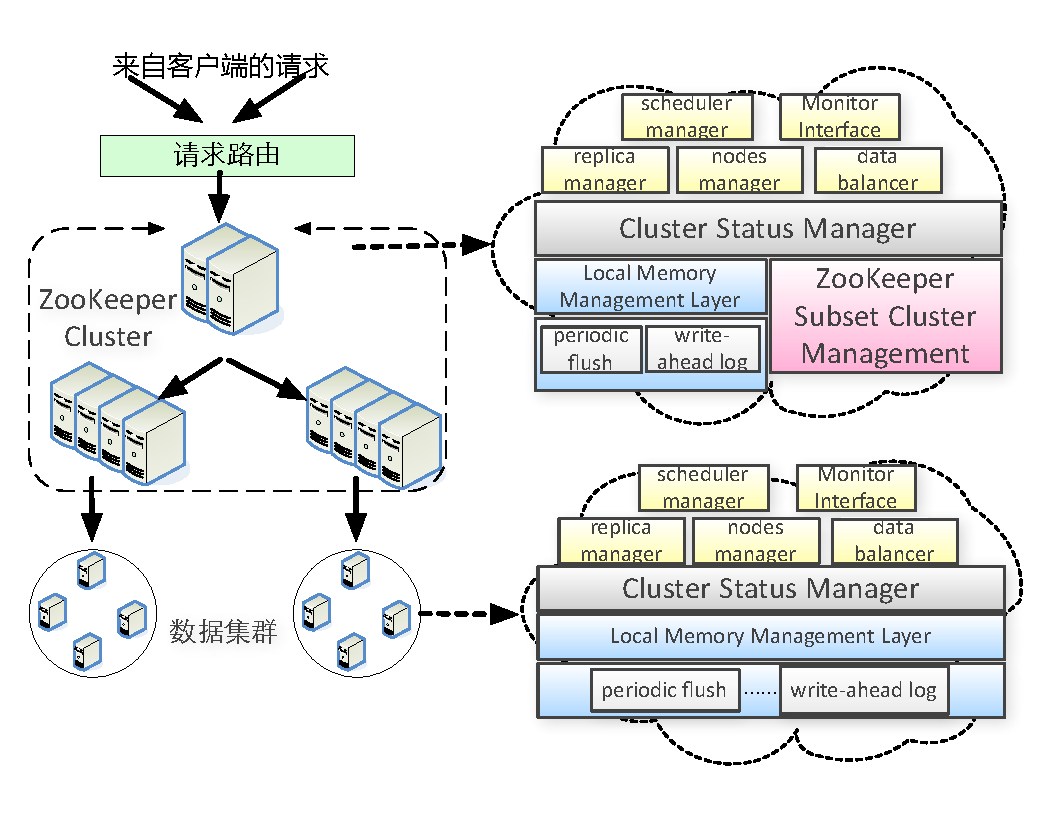
\includegraphics[width=4.5in]{../figures/logic-structure2.pdf}
\caption{Sedna机群的总体架构}
\label{fig:sedna}
\end{figure}

如图\ref{fig:sedna1},一台服务器上运行的一个完整的Sedna实例可以从逻辑上被分为本地部分(local memory store)和分布式组件(Sedna service)部分。本地部分包括本内内存管理层以及持久化存储层,分布式部分则包括了基于ZooKeeper机群一致性信息管理组件。图\ref{fig:sedna}中右侧图中,最上面的层次放置了不同的可插入组件,用来实现Sedna的可扩展的功能,比如接入不同的备份管理策略,或者接入不同的数据同步策略。

\begin{figure}[h!]
\centering
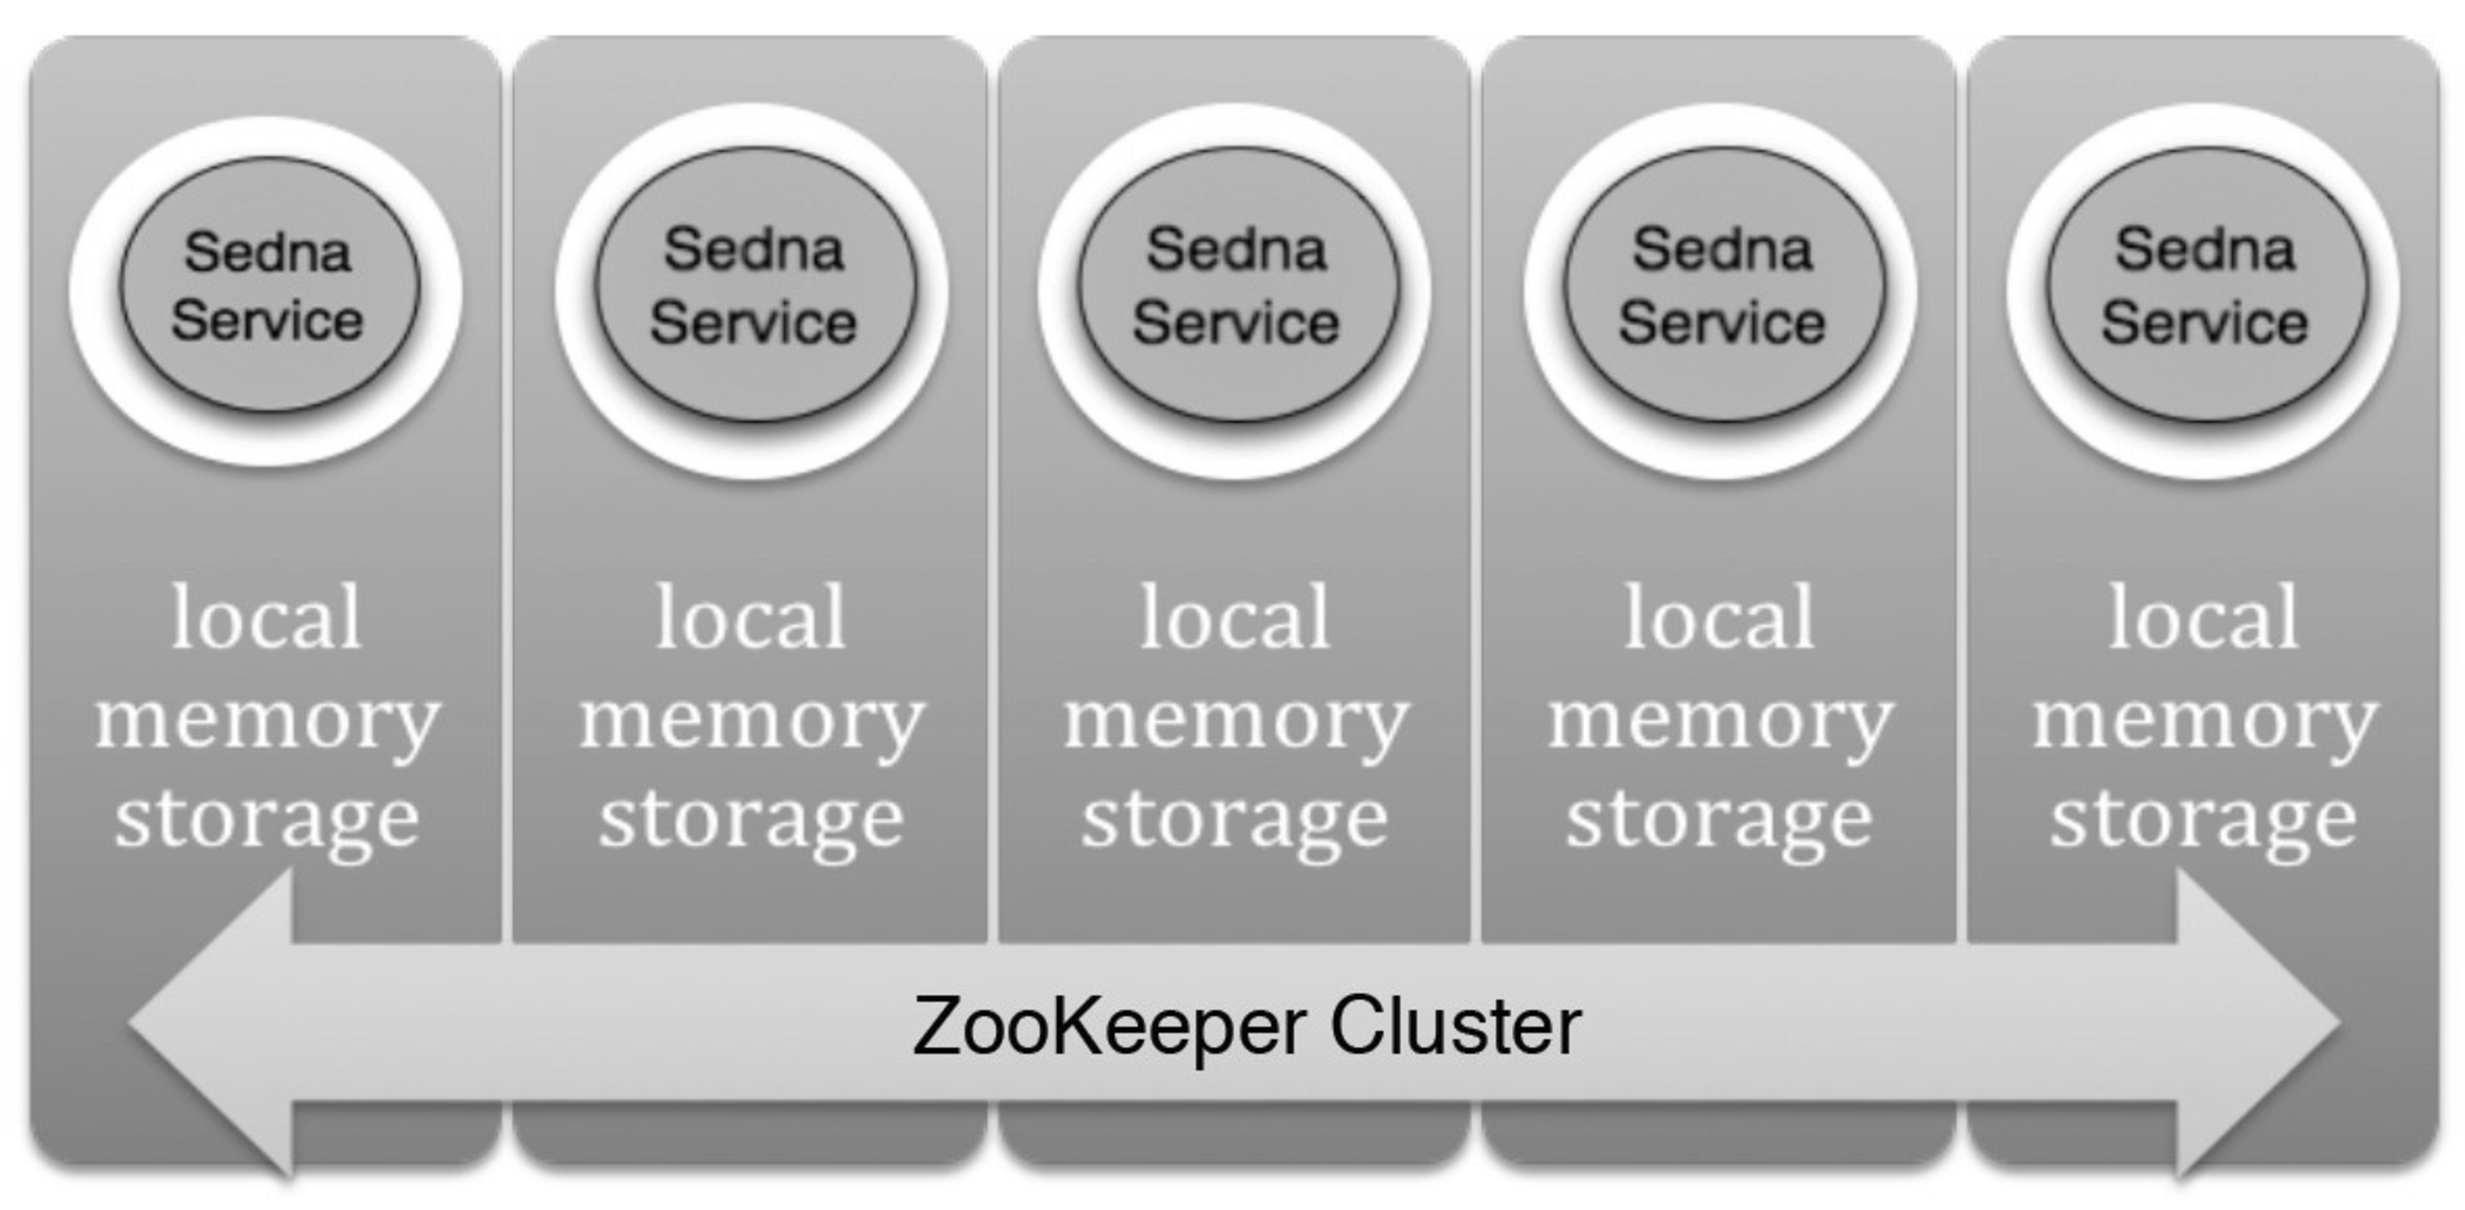
\includegraphics[width=3.5in]{../figures/SednaArc1.pdf}
\caption{每台Sedna服务器内部逻辑结构}
\label{fig:sedna1}
\end{figure}

ZooKeeper子集群是一个运行了ZooKeeper服务的集群,该集群中每一台服务器都选自Sedna集群。该子集群为Sedna提供了强一致性的分布式服务,后面我们会更详细的介绍ZooKeeper以及其在Sedna中实现的优化。总体来说,Sedna需要在下面功能处使用ZooKeeper提供的服务:
\begin{enumerate}
  \item Sedna集群在首次冷启动的时候,使用ZooKeeper的锁服务来选举一个主节
    点进行所有的初始化工作。
  \item 保存Sedna中所有虚节点和物理节点之间的对应关系。每一个物理节点都会在ZooKeeper中新建一个\textit{znode},并且将其所存储的虚节点信息写入该\textit{znode}。
  \item Sedna中物理节点的心跳信息通过ZooKeeper来维护。所有节点上的Sedna实例在初始化时都会向ZooKeeper注册一个临时\textit{znode}节点,并且向ZooKeeper维持心跳联系。当节点丢失后,ZooKeeper能够提醒Sedna处理。
  \item 所有需要多节点同步的状态都通过ZooKeeper维护。
\end{enumerate}

\subsection{数据分割}
数据分割是指将数据空间按照某种规则分割存储到分布式集群中的某一台机器的行为,它也是所有分布式存储系统首先要解决的问题。比如GFS类的存储系统可以为数据指定任意的存储节点,并且在主节点上持久的存放该位置信息,以便之后读写的时候能够找到数据的位置。在无中心节点的分布式架构中,通常使用分布式哈希算法来进行数据分割,主要原因是分布式哈希能够有效降低由于节点加入、离开系统对数据分割造成的影响。分布式哈希有多种实现方式,一致性哈希是其中典型的一种方法。经典的一致性哈希算法,如Chord\cite{stoica2001chord}中的一致性哈希算法,通过将所有的键(Key)看做是环上连续的段,将段与段的交接点看做实际的物理节点,来指派每一个物理节点存储落在它顺时针方向的端内的数据。这样,当节点加入或者退出系统的时候,都只会影响到它相邻的两个物理节点的数据存储情况。这种一致性哈希算法在集群中节点频繁变化的场景下往往会产生极度的数据分割不平衡。

Sedna是一个键值存储系统,所有的数据都以键值对的形式存储(通过对键的结构进行扩展,Sedna可以支持一定程度的数据空间划分),那么键(Key)就用来进行数据分割。Sedna使用变种的一致性哈希算法进行数据划分。该方案使用带虚节点的一致性哈希算法,并且将虚节点信息在分布式的子集群中进行集中化管理,从而极大的提高了数据分割的灵活性和节点间负载均衡度。

如图\ref{fig:vnode}所示,Sedna使用一致性哈希算法首先将整个键哈希后的区间分为数以百万计的大小相等的区间。整个哈希后的值空间为整数区间,分割后的每一个小区间都代表了一个连续的整数集。这个连续的区间称为\textbf{虚节点},每一个虚拟节点都有一个序列号。当一个键值对到来的时候,首先根据键值(Key)哈希为一个整数并且指派给某一个虚拟节点。每一个虚节点的数据都统一存储在一个服务器中(\textbf{$r1$}),并且被备份到另外两个物理节点中(如图\ref{fig:vnode}所示的\textbf{$r2$, $r3$}中)。一台服务器可能存储多个虚节点中的数据。集群中所有的物理节点被称为\textbf{实节点},以便和虚节点对应起来。

\begin{figure}[h!]
  \centering
  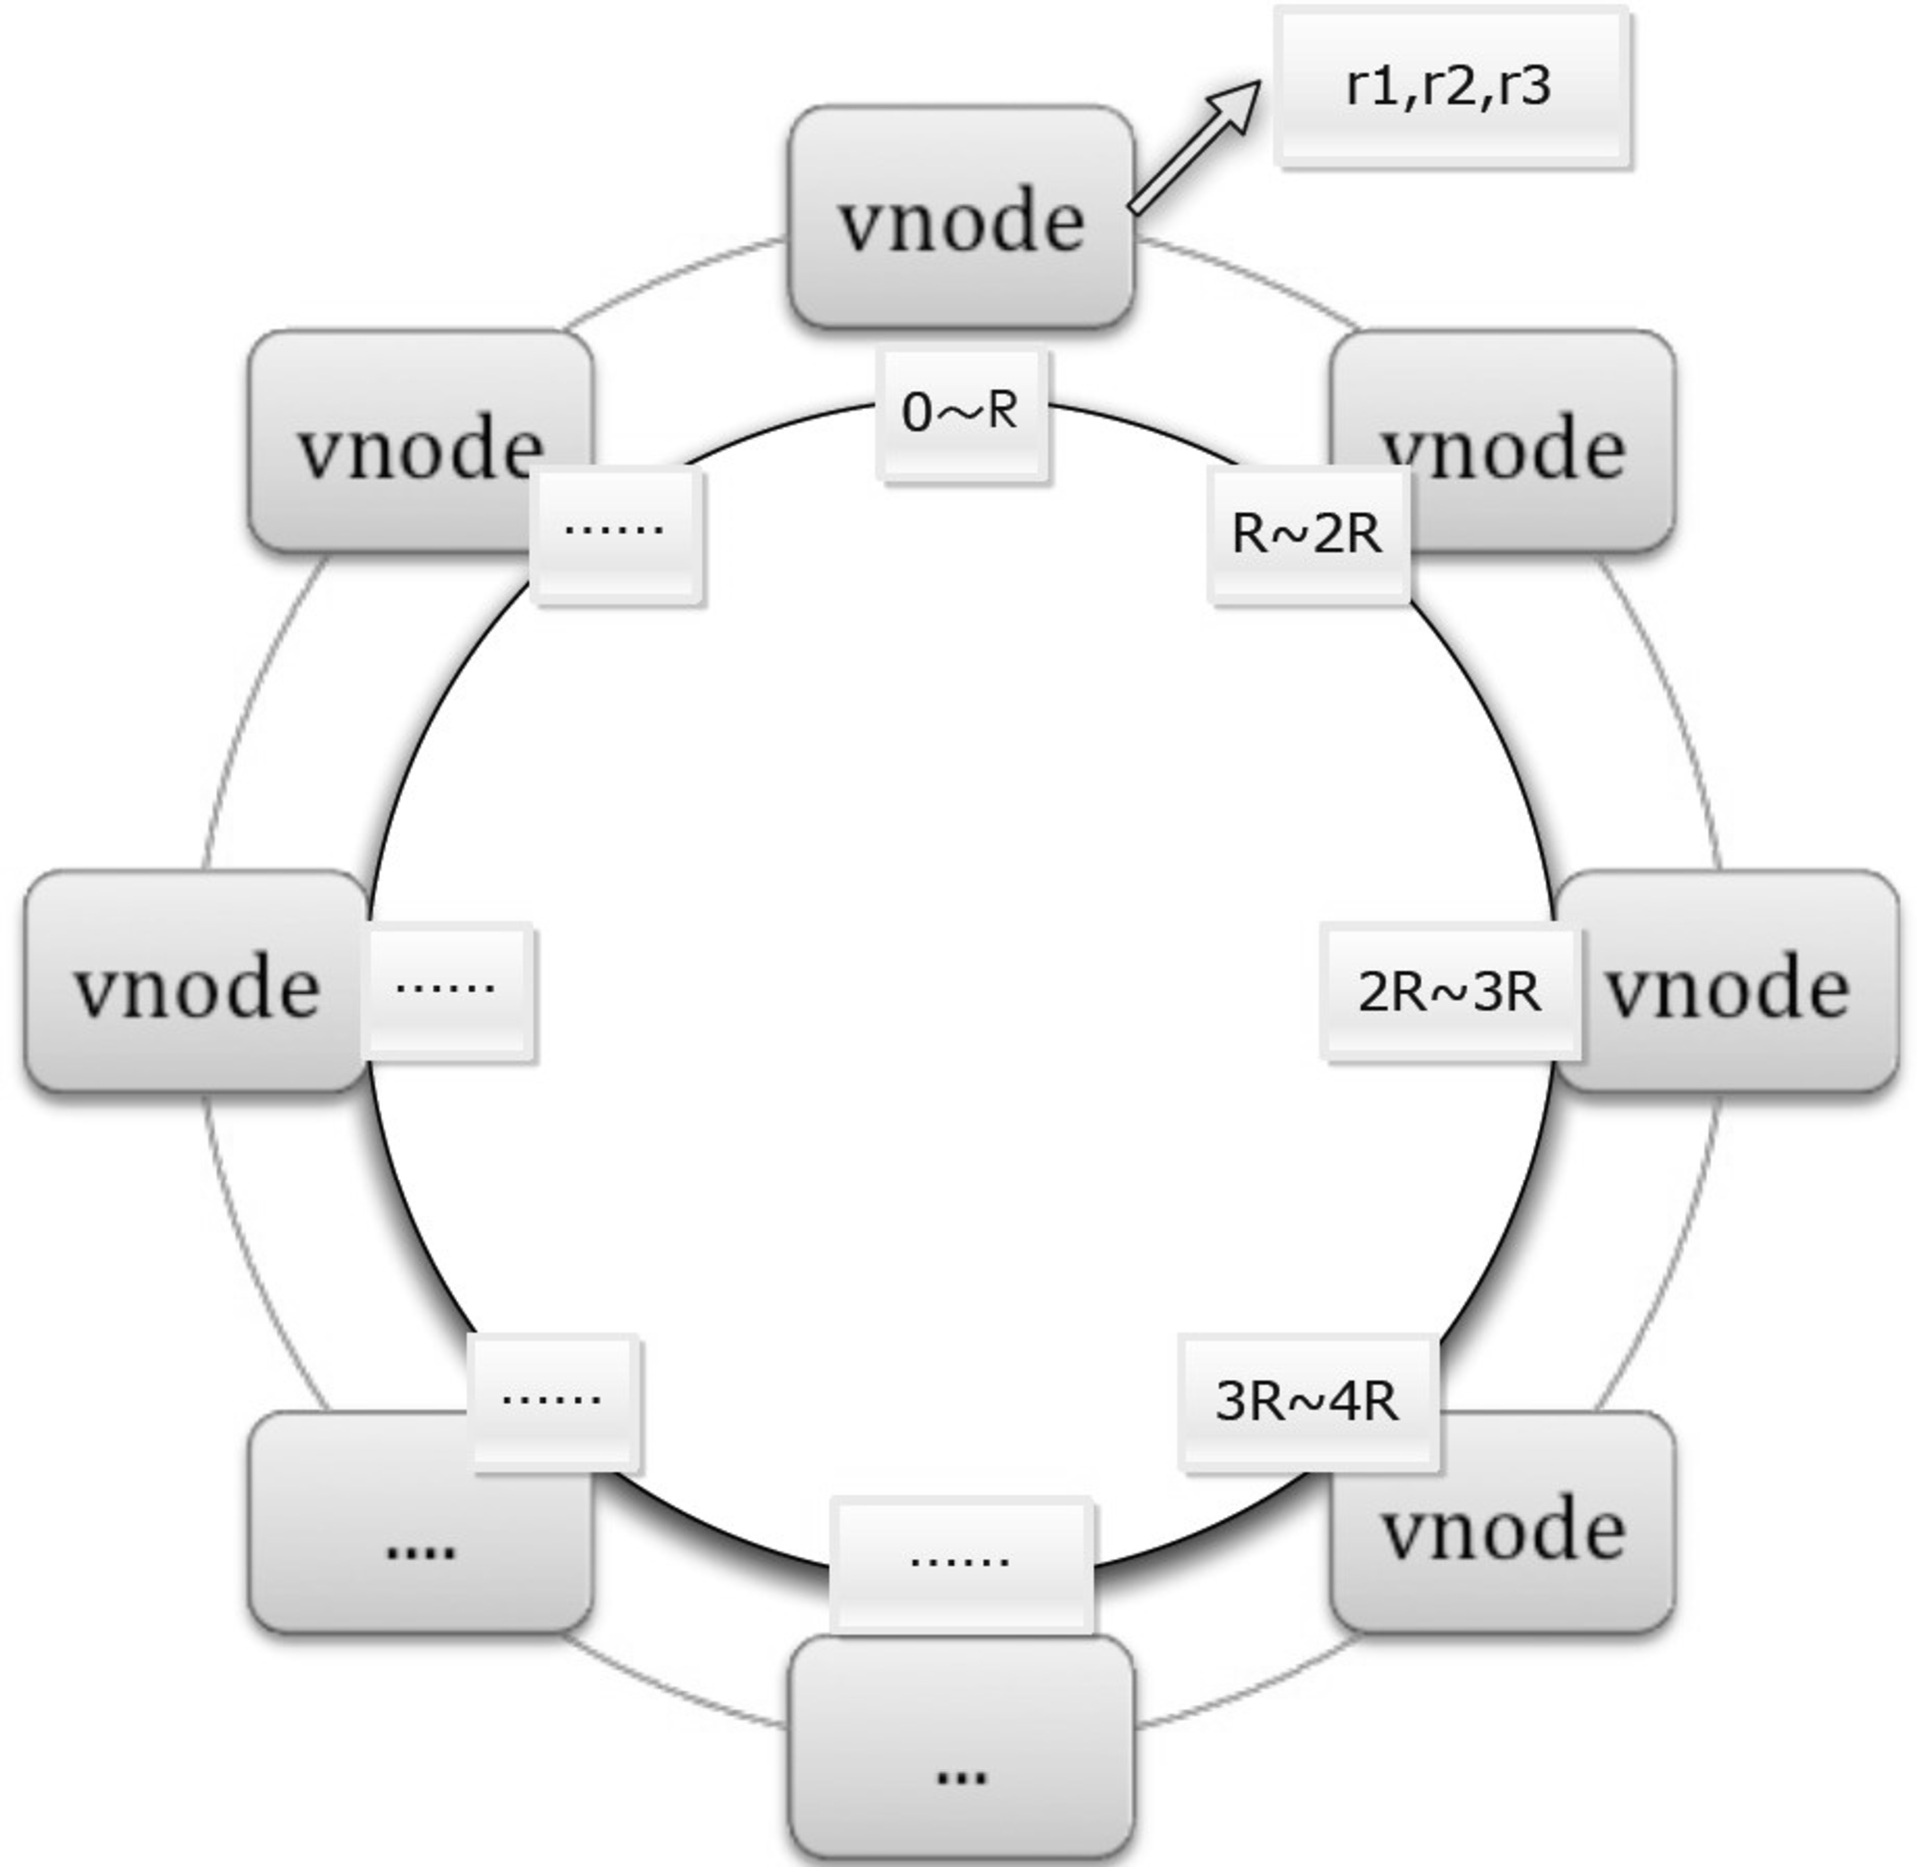
\includegraphics[height=3in]{../figures/vnode.pdf}
  \caption{Sedna虚节点环结构。其中存储着$0-R$的数据的虚节点被存储到实节点$r1$,$r2$和$r3$上}
  \label{fig:vnode}
\end{figure}

如之前所描述,基本的一致性哈希算法当面临节点不断加
入或者离开集群的时候,会导致节点之间存储的数据范围有很
大差别,从而使得集群性能不均衡,这对于构建基于有限内存的的存储集群来说问题更明显。Sedna中使用虚节点策略能够有效减少集群中数据的不均衡性:虚节点作为数据存储的最小连续块,其与访问相关的数据都会被记录下来,比如它当前存储的实际数据的容量、读写的频率等。这些信息被用来计算形成一个全局一致的实节点负载表。该负载表记录了所有存储这些虚节点的实际物理节点的负载情况。根据这个负载表,我们将数据以虚节点为单位进行数据迁移或者将新的虚节点存入负载较轻的实节点中。在Sedna中,该负载表存储与ZooKeeper子集群中,考虑到分布式读写的性能问题,均衡表不需要每次系统进行读写数据之后就更新,更新首先都是在每一个物理节点本地进行,所有的更新在本地经过计算和分析后,最终周期性的更新到负载表中。

Sedna的数据分割算法结合了一致性哈希算法和集中式的元数据管理。后者主要体现在Senda对虚节点到实节点映射信息的集中管理。Sedna中虚节点和实节点的对应关系并非像之前介绍的一致性哈希算法那样,通过在环上进行顺时针指定,该映射关系是动态可变的,可以动态改变意味着更简单的负载均衡策略,同时也意味着映射信息需要集中的存储和管理。在Sedna中,这些信息保存在图\ref{fig:sedna}所示的ZooKeeper Cluster中。这部分数据的存储和读取对系统性能影响很大,我们将在后面具体介绍它的设计和优化,并且通过实验证明该方案对系统性能的影响可控。

\subsection{数据备份}
数据备份是分布式存储系统中常用的提高数据可靠性的方法。通过将数据保存在多个服务器上,系统可以在部分节点失效的情况下继续提供数据读写服务。由于内存中的数据在掉电后无法重建,因此数据多节点备份在基于内存的分布式存储系统中更加重要。

Sedna系统中每一个数据都至少包括两个备份以保证数据的可靠性。多个备份之间由于节点崩溃,网络延迟等原因,存在不一致的可能,在Sedna中我们使用基于议会选举(quorum)的最终一致性来维护不同拷贝之间的一致性。

\begin{quotation}
假设分布式系统中,每一个节点有$N$个备份,并且假设当我们从这个$N$个备份中读取到超过$R$个一致的数据的时候,我们才认为读成功,并且返回给用户;当从$N$个备份中写入成功$W$个,才认为写成功返回。那么当$N,R,W$满足下面公式(\ref{equa:quorum})的时候,我们就可以保证每次成功读写都得到一致的结果。比如,如果每一个数据有三个备份(这也是通常情况下数据中心中备份的情况),设置$R=2$,$W=2$,此时公式\ref{equa:quorum}得到了满足,那么在这种情况下,如果一次写成功,那么就意味着至少有两个节点上已经写入了正确的结果,如果此时发出读请求,由于至少在两个节点上得到一致的结果才会返回,那么一旦返回的时候,我们可以确定返回的是刚刚写入的值。

\begin{equation}
  \label{equa:quorum}
  \begin{split}
  R + W > N  \\
  W > \frac{N}{2}
  \end{split}
\end{equation}

\end{quotation}

Sedna中的读写都是通过一个协调节点实现的,如图\ref{fig:sednareplicas}所示。来自客户端或者内部应用程序的请求通过路由器会被发送到Sedna机群中任意一台服务器,此时这台服务器就成为这次读写请求的协调者。协调者负责查询所需要的数据所在的物理节点所在的位置,并发的向存有这些数据的实节点发送请求,根据请求返回的数据的时间戳来判断是否有足够数目的一致结果。在得到足够数量的一致结果之后马上返回结果给调用者。使用协调节点能够有效的均衡客户端请求带来的压力,并且协调节点除了负责执行Quorum算法外,更重要的是还要负责起数据恢复和最终一致性的功能。

\begin{figure}[h!]
\centering
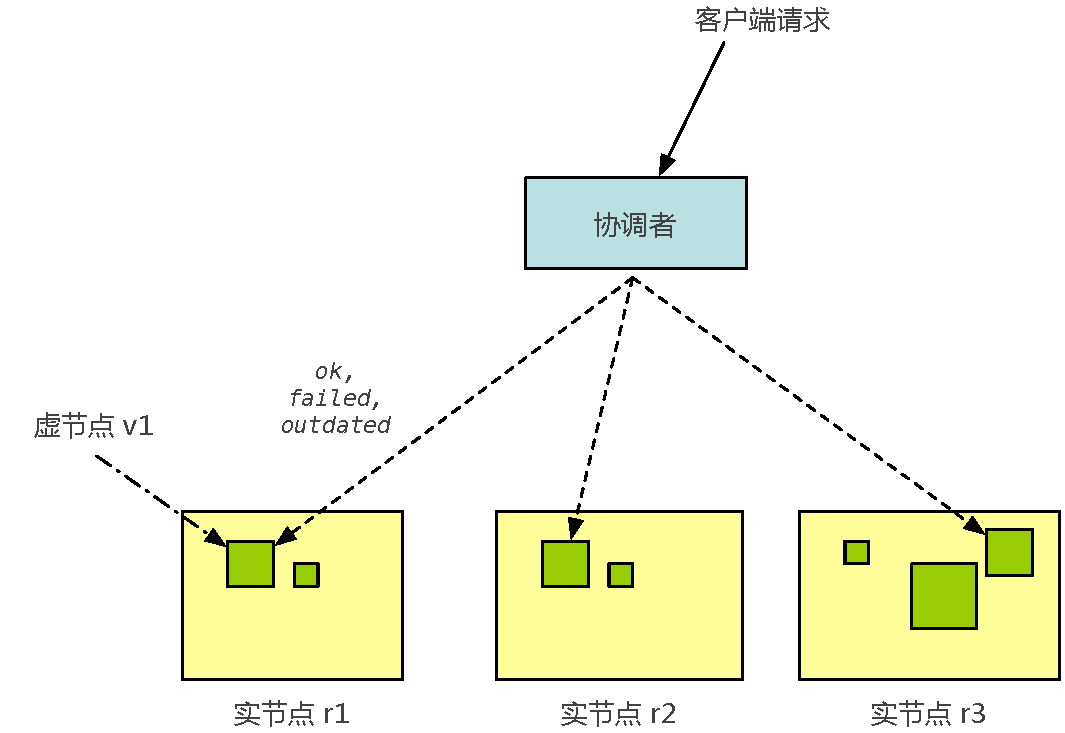
\includegraphics[width=5in]{../figures/sednareplicas.pdf}
\caption{Sedna使用协调者进行多备份读写过程}
\label{fig:sednareplicas}
\end{figure}

为了保证数据的可靠性,Sedna中每一个数据保持了多个备份。对一个集群来说,服务器离线重启再上线的情况会经常发生,因此系统中经常出现备份不足或者备份之间数据不一致的情况。Sedna并不强制要求每一次读写过程中所有的数据都一致,而是采用了最终一致的策略:对于那些数据不一致的节点,Sedna会启动异步的过程对其中数据进行强制同步,这个修复过程发生在\textit{数据读}的过程中,我们称为\textit{读恢复}。读恢复发生在协调节点上。当协调节点向多个备份发送读请求的时候,那些离线或者崩溃的节点会出现超时的情况(如图\ref{fig:sednareplicas}所示)。按照Quorum算法的要求,对于达到了公式\ref{equa:quorum}的读写请求,但仍有部分节点返回不一致的数据的情况,协调者在返回给客户端正确的请求数据之后会开始数据恢复工作。

对于超时或者拒绝服务的返回值,协调节点会再次向ZooKeeper集群确认该节点是否离线或仅仅是协调者本身出了问题。如果确认对方节点确实已经离线,协调节点会异步的启动一个数据备份任务,将数据从已存的物理节点中拷贝到新制定的节点中去,并且在拷贝完成之后修改数据的映射信息。

\subsection{节点管理}
节点管理主要包括:1)对集群中的现有节点的状态进行监控,及时发现节点失效的问题,并采取对应的措施;2)对新加入集群的节点进行管理,进行数据迁移,维持集群的负载均衡;3)对由于软硬件错误离开集群的节点进行管理,维护集群的稳定性。

Sedna对于节点加入和退出都是自动处理的。如果集群中新加服务器,只需要在其上启动Sedna实例即可。如流程图\ref{fig:sednastart}所示,每一个刚启动的Sedna实例都首先启动本地的内存管理模块,之后申请连接ZooKeeper Cluster来同步状态。如果ZooKeeper服务还没有初始化完成,这意味着整个Sedna集群还没有启动,该Sedna实例会申请一个全局锁,并初始化整个集群。对于ZooKeeper已经成功启动的情况,所有新加入的节点都会通过在ZooKeeper的$real\_nodes$目录下创建一个临时Znode节点($ephemeral$)来表明自己的存在;完成后,本地会启动一定数目的线程(根据及其性能来配置)来从当前负载较高的服务器上请求虚节点数据,并且存储到本地。当该动作完成后,它会改变集群中虚节点到物理节点的映射关系。因此它需要最后向ZooKeeper子集群申请修改这部分数据。在Sedna中,虚节点的数目是在集群启动前写入到配置参数中的,一旦集群启动后,不能够更改。节点在加入系统之后会启动一定数目的线程来从别的物理节点拉取数据,这个线程数目可以根据虚节点的数目进行调整。

\begin{figure}[h!]
\centering
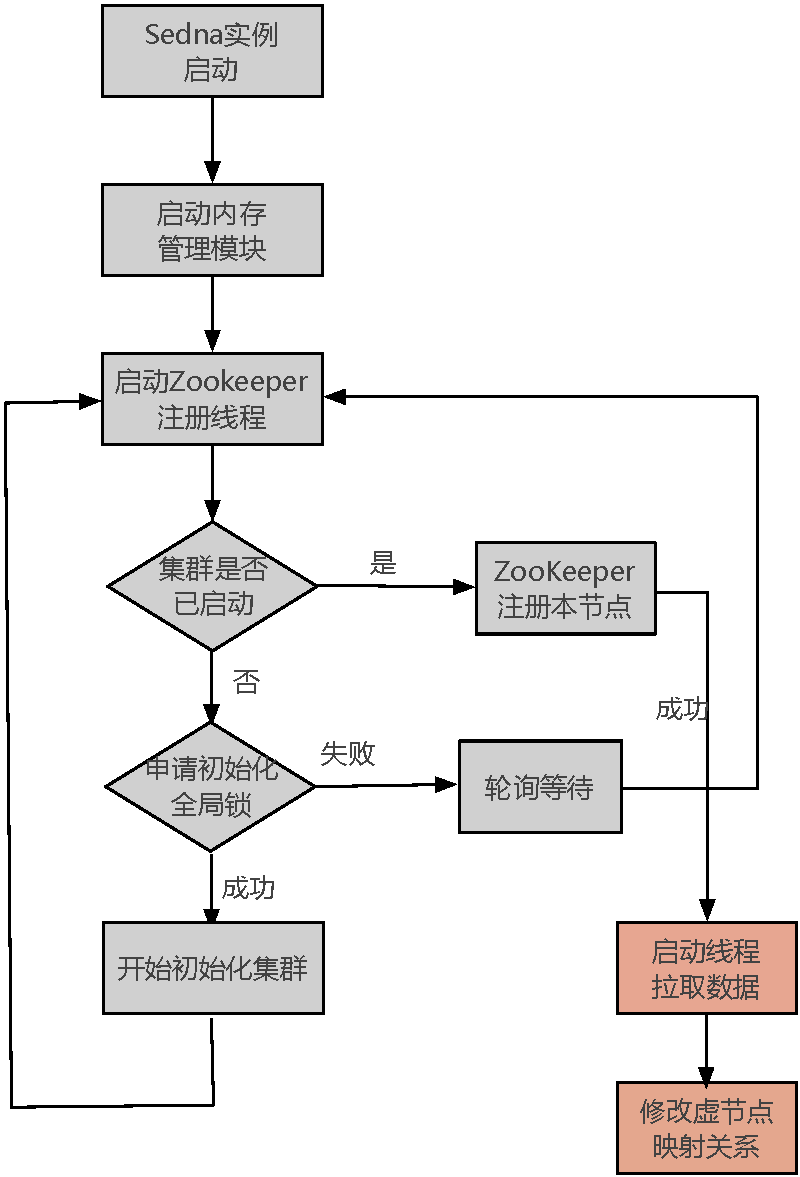
\includegraphics[height=4in]{../figures/sednastart.pdf}
\caption{Sedna中节点加入服务的流程图}
\label{fig:sednastart}
\end{figure}

当一个节点意外的离线或者崩溃的时候,之前维持的节点和ZooKeeper集群之间的心跳信息丢失。这个动作会提醒ZooKeeper有节点离线了。此时Sedna集群并不会立即做出反应,节点丢失的恢复工作主要由读操作的时候指派的协调者来执行。

\subsection{ZooKeeper子机群}
Sedna使用Zookeeper\cite{hunt2010zookeeper}子集群来实现分布式锁及元数据管理。Apache Zookeeper是一个开源的用于开发大规模分布式程序中分布式协调的组件。它是一个中心化的服务,可以用来存放全局一致的配置信息、名字空间信息、提供分布式的同步或者组服务。ZooKeeper是基于ZAB(ZooKeeper Atomic Broadcaset)\cite{junqueira2011zab}协议的,ZAB是一种类似Paxos的分布式一致性协议,其性能好于现有的Paxos\cite{lamport2001paxos, lamport2006fast}实现。

ZooKeeper服务会在Sedna集群的一部分节点上运行,这部分节点就构成了图\ref{fig:sedna}中的ZooKeeper Cluster。该子集群中节点的数目可以根据Sedna集群规模变化而变化。ZooKeeper Cluster在Sedna中的作用非常重要,本节中我们将分析Sedna中ZooKeeper的使用,并且针对性的设计优化的策略。

图\ref{fig:zkper}展示了ZooKeeper版本3.2运行在拥有双核2Ghz的Xeon以及双SATA磁盘上的性能图。读请求共1K个,写请求也为1K,服务器(Servers)表明了Zookeeper所管理的服务器数目,除了这些ZooKeeper服务器外,试验中采用了超过30个额外的的服务器模拟客户端请求。

\begin{figure}[h!]
  \centering
  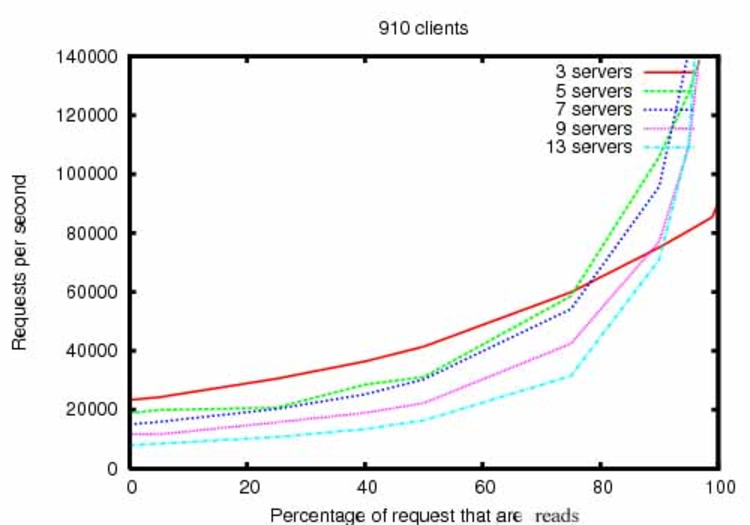
\includegraphics[width=3.5in]{../figures/zkp.pdf}
  \caption{ZooKeeper性能随着读写比率变化图}
  \label{fig:zkper}
\end{figure}

通过上述试验我们给出ZooKeeper的性能特点总结:

\begin{enumerate}
\item 请求中读占的比重越大,ZooKeeper集群能够响应的请求数目越多。
\item 对于读请求,ZooKeeper的性能随着服务器数目的增加而提升;对于写请求,性能反而会随着服务器数目的增加而降低。
\end{enumerate}

这两点很容易理解,因为客户端读数据的时候仅仅需要连接ZooKeeper集群中任意一台服务器即可。但是写请求需要传播到ZooKeeper集群中的多台机器,从而使得效率较低。根据上面优缺点可见ZooKeeper本身是一个写效率较低而读效率较高的系统,因此在Sedna中对ZooKeeper将尽量使用读而不是写,需要写的主要有两种情况:

\begin{enumerate}
  \item 当Sedna集群首次启动的时候,所有的物理节点都需要向ZooKeeper创建代表自己的\textit{znode}。除此之外,负责初始化的节点首先还需要单独向ZooKeeper写入代表所有虚节点的\textit{znode}。典型的Sedna配置中可能包括数百万条虚节点,因此这些动作会产生大量的写操作。
  
  \item 当物理节点加入或者离开集群的时候,Sedna会自动更新系统中表示物理节点的znode的数据。当我们因为数据均衡或者数据一致性需要对数据进行迁移的时候,需要修改虚节点和物理节点之间的对应关系,这是通过写ZooKeeper中数据实现的。
\end{enumerate}

前一种情况虽然非常耗时,但是由于其只会在集群启动的时候执行一次,因此我们不会将其作为性能瓶颈来考虑。后一种情况在系统运行时会时有发生,但是以ZooKeeper毫秒级的写速度,这种情况即便发生也不会对Sedna的性能产生明显的影响,这在实验中也得到了验证。

ZooKeeper的读性能是Sedna的另一个性能瓶颈。为了避免这个瓶颈,我们使用了如下三个策略:1)大量使用本地缓存。Sedna中协调者进行读写操作的时候优先从本地缓存中获取数据,当缓存数据被证明失效的时候才会从ZooKeeper中更新新的数据。2)为了减少由于缓存失效带来的长时间延迟,我们在每一个Sedna实例中还会启动一个周期线程负责从ZooKeeper中更新数据的映射信息。该线程执行的周期称为\textit{租约时间}。租约时间是不断变化的:当最近对于ZooKeeper中的数据有写入,那么租约时间就会减半;如果在上一个租约时间内ZooKeeper中没有数据改变,那么下次租约时间就会延长一半。3)每次对ZooKeeper中数据进行更新的时候,系统会将其记录在单独的\textit{znode}目录下,这样无论在写入和读出的时候都能够避免锁,其次在ZooKeeper中我们关闭监控(watch)功能以防止因为大量的节点监控同一个znode节点,导致的该节点上任何一个改变引发大量线程突然启动的惊鸿效应。

\subsection{基本数据访问API}
\subsubsection{写操作}
由于在web2.0应用中,随机写是一种非常普遍的操作,Sedna存储系统允许来自不同客户端对相同的键进行无锁并发写操作。Sedna中所有的键值对数据都有时间戳的保护,并且每一个键所对应的值都不是单一的一个值,而是一个列表,列表中保存了来自不同的协调者所写入的最新的值以及当时的时间戳,列表的第一个元素则维护着来自不同的协调者写入的所有数据中时间戳最新的那个值。Sedna为写操作提供了两个不同的API:\textbf{write\_latest()}和\textbf{write\_all()},他们两个都是无锁写。

用户调用\textbf{write\_lastest()}函数时,Sedna会将请求的时间戳和当前该数据最新的时间戳进行比较,对于试图以较旧的时间戳更新当前较新的数据的请求会返回一个$outdated$,而那些具有更新时间戳的写请求将直接覆盖当前数据,并且返回给用户$ok$。而如果用户调用\textbf{write\_all()},那么Sedna只会将请求的时间戳与该数据上次来自相同协调者所写的版本号做比较。如果当前请求比较新的话则会更新那个来自,否则返回$outdated$。

任何程序调用写API都会得到三个不同的返回值(如图\ref{fig:sednareplicas}所示):$ok$代表当前数据被成功写入并且覆盖原有数据;$outdated$表示当前数据比较老,未能覆盖掉原有数据;$failure$表示由于网络等原因写失败。

\subsubsection{读操作}
键值存储系统的读API都非常简单,给定一个键,返回当前键对应的数据。由于Sedna中所有的值都根据它们来源和时间戳进行管理,我们也对应提供了\textbf{read\_latest()}和\textbf{read\_all()}两个API给应用程序快速的获取值。如字面意思所示,\textbf{read\_latest()}会返回最新的数据,不管当前读操作所在的协调者是什么状态;而\textbf{read\_all()}则会返回当前键对应的来自不同协调者写操作的所有数据,这些数据被维护成一个列表发送给客户端。如何处理这些数据的不一致将是客户端软件的工作。

\subsection{持久化策略}

Sedna实现了两种不同的持久化策略:周期刷新和写前日志。写前日志不是默认的持久化方式,它只是对于特定的应用可以启动,用来应对非常严格的数据持久化要求,而周期刷新作为日常情况下数据的持久化策略,已经足够保证Sedna中数据的高可用性。

我们首先分析一下周期刷新策略的可用性。在一个有$n$个服务器的集群中,假设所有的节点都有相同的MTBF\cite{mtbf}值为$m$,那么每一个服务器在时间间隔$t$内发生失败的概率为$\frac{t}{m}$。如果当前Sedna集群中共有$v$个虚节点,那么从某一个虚节点中读取数据的概率为:$\frac{1}{v}$。假设周期刷新的周期为$T_{f}$,以及整个Sedna集群
的读写的带宽为$tp/s$.

Sedna出现丢失数据的条件是比较苛刻的,它要求:1)一个数据的三个备份都在短时间内发生故障;2)其次这个时间段内没有发生过任何数据刷新到磁盘的动作;3)并且这个时间段内也没有任何来自客户端的对该失效节点上任何一个虚节点进行访问。那么发生这三个事件的概率是可以计算的:

\begin{displaymath}
P_{f} = (1 - \frac{1}{v})^{tp* T_{f}}(\sum_{i=3}^{n}  (\frac{T_{f}}{m})^{i} (1- \frac{T_{f}}{m})^{n-i} ( 1 - \frac{C_{v}^{ik} C_{ik}^{k}\cdots C_{2k}^{k}}{(C_{v}^{k})^{i}}))
\end{displaymath}

根据上面的公式所示,$P_{f}$是一个非常小的数。假设一台服务器的
$m=50,000$小时,$n=1,000$,并且$T_{f}=600$,那么$P_{f}$小于
$2e^{-20}$. 因此我们认为在Sedna中使用三个备份,并且周期性的将数据刷新到磁盘中的方案在统计意义上来说是足够保持数据的可靠性的。


\subsection{Sedna实时数据访问接口}

Sedna是为实时应用设计的分布式存储系统,除了将数据完全放入内存中来提高系统的读写速度外,设计了新型的基于层次的存储架构来提高系统的扩放性外,更重要的是Senda实现了一套实时数据访问接口帮助用户编写复杂的实时应用。

为了支持用户多种多样的实时应用的需求,Sedna增加了基于触发的API作为其基础功能。触发适合实时处理的关键在于,它对于数据的更新极为敏感。每当数据发生变化的时候,触发快速执行需要的动作,能够很快的给出用户需要的结果。触发机制在数据库中作为辅助工具已经广泛使用多年,这些功能在数据库中往往是作为确保数据完整性、合法性检查而出现的,不过我们在Sedna中设计的触发API和数据库中的触发器还有所不同,主要差别体现在Sedna运行在大规模的分布式集群中,其面临着更加复杂的调度和管理任务:不断执行的多个触发之间如果有相关性的话如何在存储层进行控制,如何帮助上层应用进行负载均衡等。

一个基于Sedna的触发API实现的典型的实时应用程序通常包含了若干个对数据的触发访问来完成计算任务。如图\ref{fig:triggers}所示,我们用三个触发器A、B、C来构成一个计算任务。触发器A会监测初始数据集的并且产生中间结果写入Sedna系统中,这些中间结果的改变会触发触发器C执行,C执行的结果会导致触发器B执行,而B最终将再次触使A执行。以此往复。A、B、C共同构成了一个循环任务的三个子部分。

\begin{figure}[h!]
  \begin{center}
    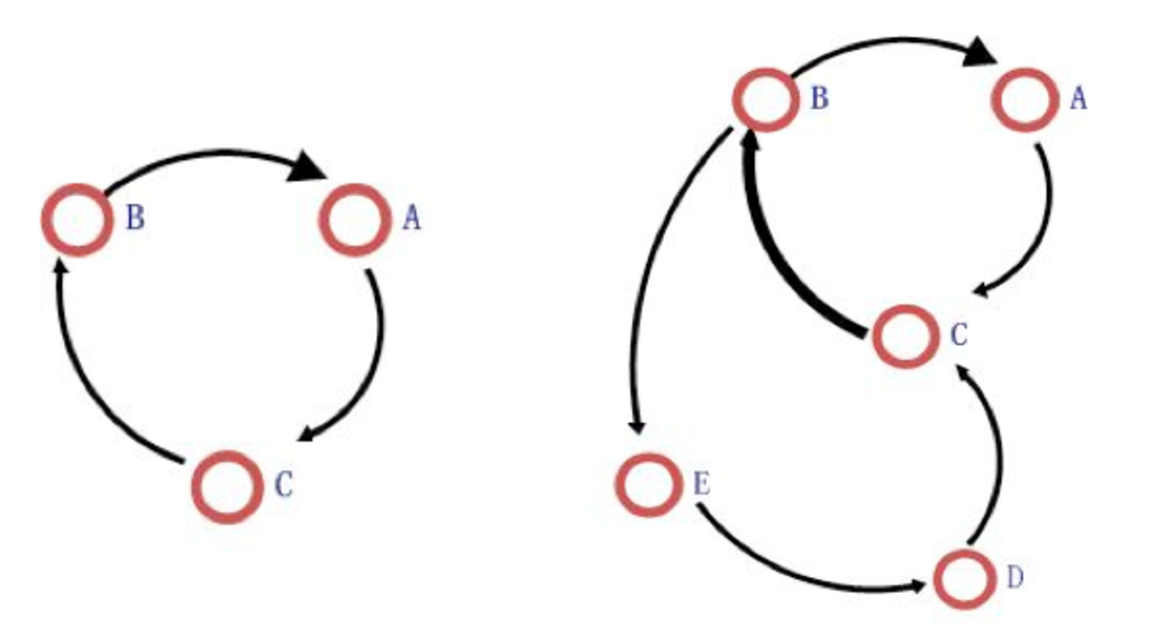
\includegraphics[width=4in]{../figures/domino.pdf}
    \caption{Domino提供的基于触发的实时数据访问接口的典型应用实例}
    \label{fig:triggers}
  \end{center}
\end{figure}

\subsubsection{流控制}
Sedna中基于触发的API简单易懂,然而在一个分布式存储中广泛的提供这种API却面临着种种问题,其中最重要的挑战在于如何解决由多个触发API调用带来的可能的涟漪问题。我们依然使用图\ref{fig:triggers}来描述这个问题。图\ref{fig:triggers}中右图展示了Sedna之上的应用调用了A-E共5个API,我们称应用使用了5个触发器A-E。执行过程中,A、D两个触发后执行的结果一步激活了触发器C,而C的执行结果反过来又导致A和D的执行,由触发器相互激活形成的环可以用来支撑一些复杂的应用,然而在本例中,一旦循环开始,每一轮下来所有触发器被激活的概率都会提高一倍并且最终将整个集群的资源占完。并且由于Sedna是作为一个存储系统存在的,多个独立的用户会共同使用同一个集群,由于互相之间并不了解对方的应用,因此出现这种情况的概率就更高了。我们通过在Sedna的触发API中引入token机制来平衡触发执行的速率。每一个触发器的执行都需要一定的周期来获得token,对于那些在没有获得token的时候数据更新,API将会自动忽略,并且不会返回数据给用户程序。下面的代码展示了如何利用Sedna的实时API编写一个简单的应用(基于Java)。由于Java不是函数语言,所以开发者需要将执行的动作封装成一个简单的Java类,并且提交给Sedna实时API。对于Sedna的实时API来说,每次调用都需要指定API所监控的键或者键的范围,数据发生改变时需要接管的类。每一个传给实时API的类都必须是Action类的子类,其中关键的action函数将获得新写入的数据的值,并且负责进行处理。

\subsubsection{Sedna实时API应用的示意}
\begin{lstlisting}[language=java]

public class myAction extends Action<Key, Iterator<Value>, Result>{

  protected void action(Key k, Iterator<Value> vs, Result){
    //user codes here
  }

  protected boolean filter(){
    //user codes here
  }

  public static void main(String[] args){
    SednaClient instance = new SednaClient();
    instance.ReadTrigger(KeySet, myAction.class);
  }
}
\end{lstlisting}

在上面例子中,首先我们实现了一个Action的子类myAction来负责执行用户逻辑,并且在主函数中调用SednaClient的实时触发API($ReadTrigger$),其中指定了需要处理的键的范围以及执行的动作类。在示例中还有一个filter函数,该函数也是Action基类中的函数之一,用户应该继承它来根据自己的需求设置停止条件。Filter机制基本包括两个方面:其一,filter函数是基于每一个键值对来调用的,Sedna运行时系统会根据filter函数是否返回true来决定是否执行用户动作;第二是filter函数使用的参数中包括了当前改变的数据以及改变前的数据,这样设计使得很多迭代收敛的任务能够更容易的基于Sedna实现。

\section{实验和性能分析}
\label{section:exp3}

本节中我们将对Sedna存储系统的性能进行实验分析。在Sedna中,我们使用了修改版本的Memcached作为本地内存存储,因此它的性能受到Memcached性能的限制。然而通过跟Memcached的性能比较我们可以看出,即便作为一个分布式的存储系统,Sedna依然具有和Memcached可比的性能特征,并且能够提供Memcached这类缓存系统所不具备的持久性、扩放性等特征。在试验中,我们并没有将Sedna和别的基于内存的键值数据库来比较,比如MemBase\cite{membase},主要原因是这些系统的并非基于Sedna所依赖的Memcached实现的,并且设计的主要目标也不同,使得这种比较不够公平。我们相信,通过和广泛应用与业界的Memcached性能进行比较,我们能为Sedna系统的性能设定一个标准的比较值。别的系统通过和Memcached性能进行比较就可以相比较出和Sedna的性能差别。

本节所有试验都基于一个有9台物理服务器的实验集群,其中每一台服务器都
使用Xeon双核2.53Ghz处理器以及6GB的内存。所有的物理机器都通过一个GB的以
太网互联,节点之间没有划分机架,所有节点之间的消息传递的时间在毫秒以内。
所有Sedna实例服务器分为两种,一种单纯运行数据存储功能,我们为每一台节
点预先开辟4GB内存作为本地数据存储;另外一种节点构成了ZooKeeper子集群,
因此其上还需要运行Zookeeper服务,我们为每一台节点开辟3GB内存存储本地数
据。同时我们还使用Memcached在相同的实验集群上配置了相同的内存容量来进
行比较

\subsection{单客户端性能}

在本测试中,系统中只有一个客户端分别对Sedna集群和Memcached集群来进行
读写请求。所有要存储的键值都非常小,因为数据的大小并不是影响Sedna系统
性能的核心因素,数据大小仅仅会对网络带宽有影响。为了让所有的测试可比较,
我们每次都随机产生一个20字节的键,比如$test-000000000000000$,以及一个
20字节大小的固定值写入Sedna中。

\begin{figure}[h!]
  \centering
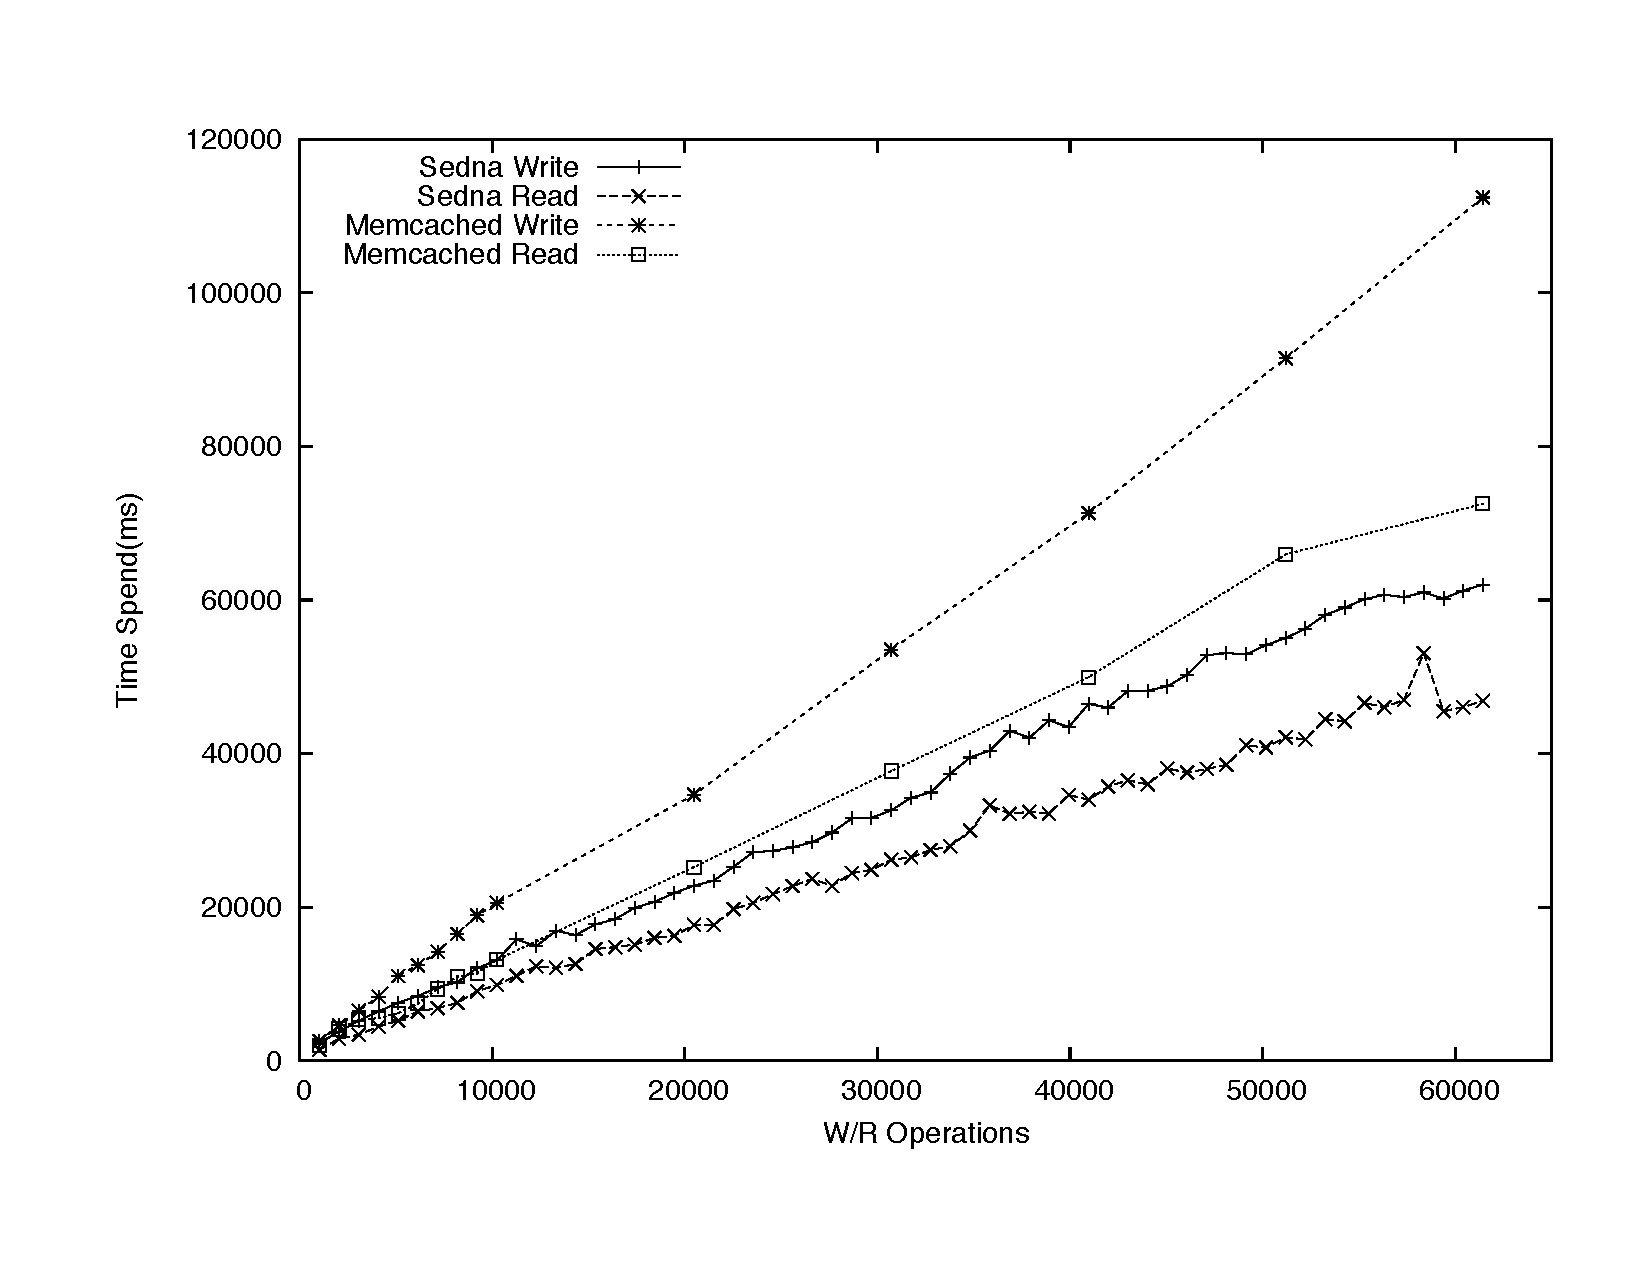
\includegraphics[width=5in]{../figures/compare_one_client_memcached_three.pdf}
\caption{Memcached客户端向不同的节点读写三次数据和Sedna正常读写的性能
  对比}
\label{fig:cp1}
\end{figure}


前面我们也描述了,为了给出比较标准的对比性能,方便与其他存储系统做比较,
所有的试验都以Memcached作为标杆。运行分布式的Memcached集群不需要在服务
器端做任何的配置,很多Memcached的客户端本身就支持以一致性哈希的方法将
数据分割到不同的节点上去。当然了,Sedna本身作为一个支持持久存储的内存
存储系统,它和Memcached这样的缓冲系统还是有一个非常重要且会影响性能的
区别的:Sedna会将一个数据并发的向不同节点写入至少3处,并且在其中2处返
回成功的时候返回。而Memcached只需要写入一份数据即可。为了使得这两个系
统的比较更加清晰,我们先后强制要求Memcached的客户端读写三次数据和读写一次
数据与Sedna读写请求做一次对比,最终的结果如图\ref{fig:cp1}和
\ref{fig:cp2}所示。

\begin{figure}[h!]
  \centering
  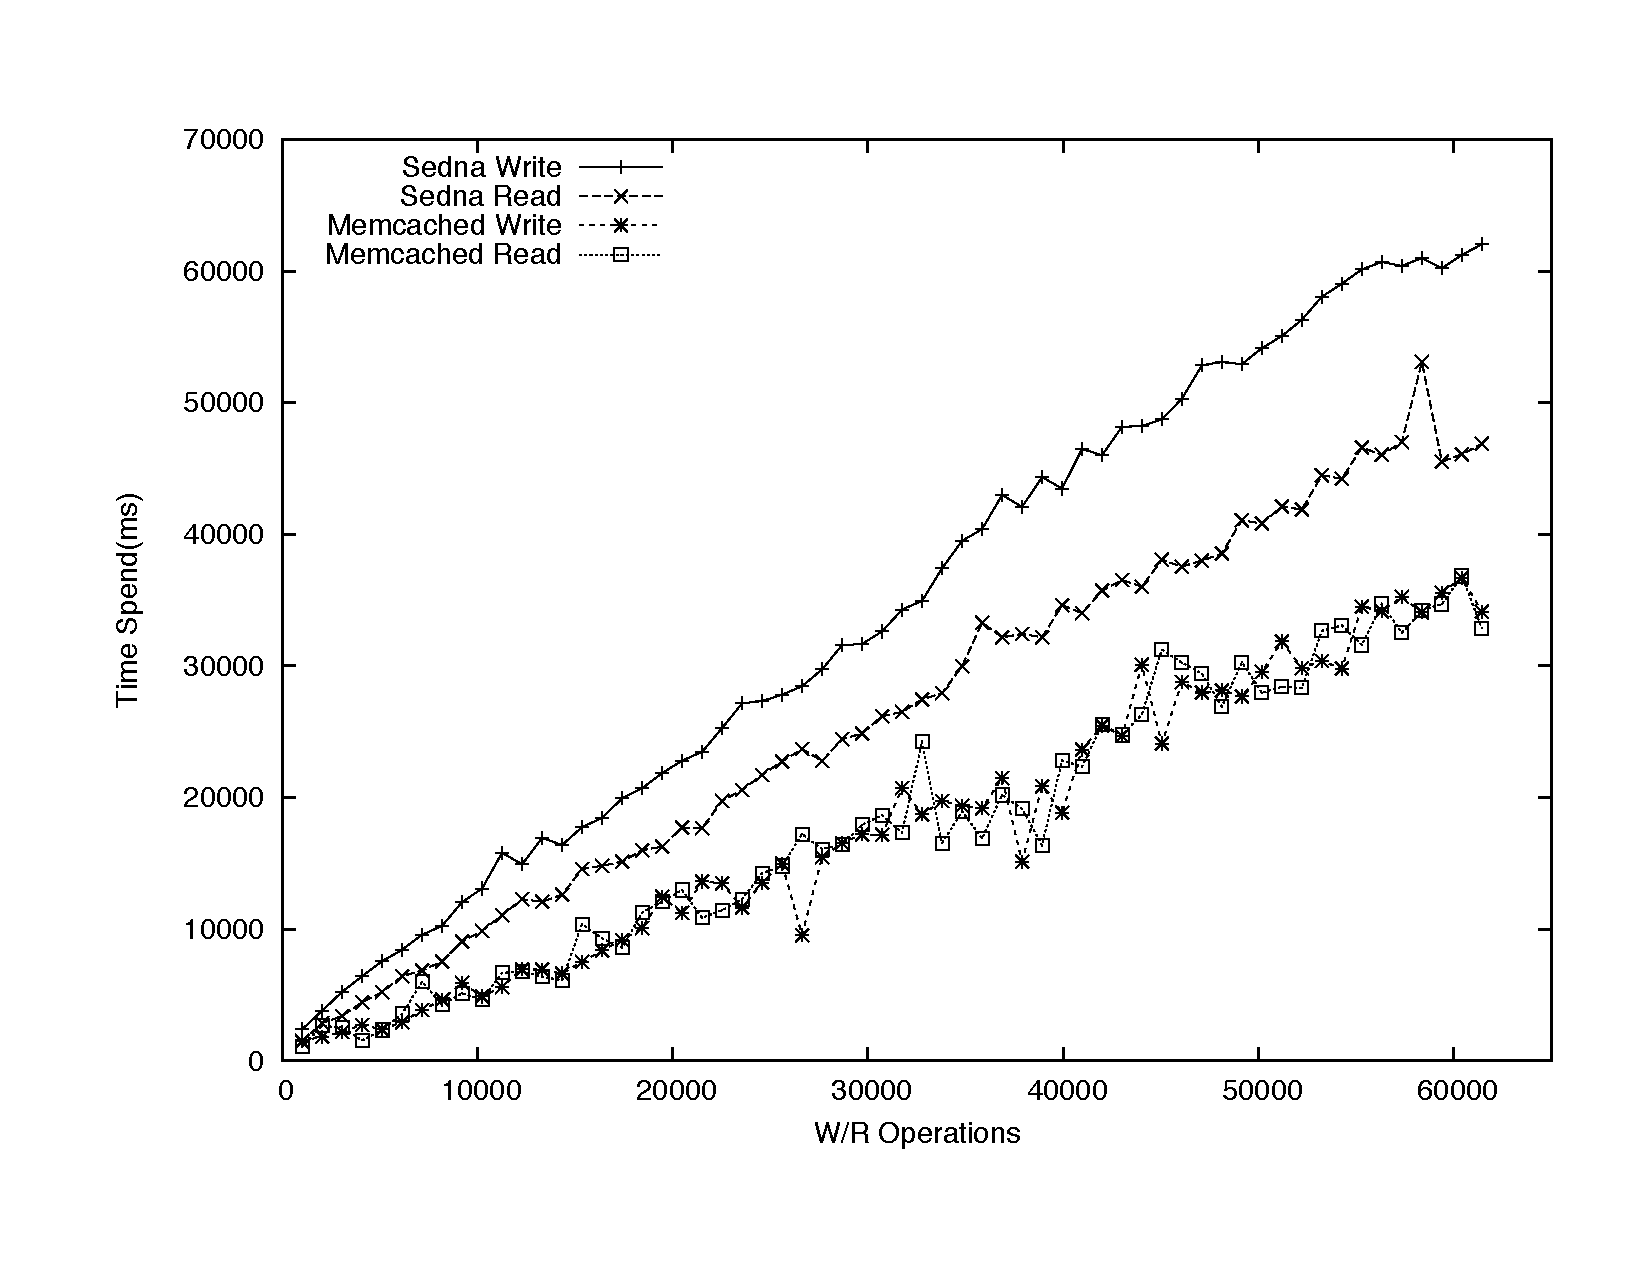
\includegraphics[width=5in]{../figures/compare_one_client_memcached_one.pdf}
  \caption{Memcached客户端向不同的节点读写一次数据和Sedna正常读写的性能
    对比}
\label{fig:cp2}
\end{figure}

尽管从图\ref{fig:cp1}中显示Sedna的读写性能都优于Memcached,实际上这里
面有一些不公平的地方:Memcached的三次读写是顺序进行的,而在Sedna中,我
们使用并发读写,并且使用了Quorum算法使得不需要等待最慢的读写完成,因此
性能要优于Memcached。之所以没有为Memcached设置并发读写,原因主要是如果
用户需要使用多次写入不同节点来保证数据的安全性,在客户端往往是通过依次
写成功来保证的。除此之外我们还在\ref{fig:cp2}中比较了Memcached只读写一
次的性能和Sedna的对比,可以看出来Sedna的性能比较稳定,一直保持高速的读
写能力,并且其速度比单纯memcached缓存系统稍慢,却明显快于在memcached中
用client实现多备份的做法。

\subsection{多客户端性能}

作为一个云计算平台下的分布式存储系统,通常不只一个客户端在进行读写请求,
系统中可能同时存在大量的应用从不同的节点请求读写。本节中,我们将在
每一个服务器上启动一个客户端同时发起读写请求。在这种情况下,网络带宽有
可能成为系统的性能瓶颈,在我们的试验中,所有的服务器都通过1GB以太网互
联。

图\ref{fig:perf}展示了9个客户端同时请求时Sedna的性能,图中的读写次数是
所有客户端读写速率的平均值。我们可以看出随着客户端数目的增加,每一个节
点的IO性能都有所下降。这很容易理解,因为多客户端导致的服务器负载增加,
网络带宽拥塞等。考虑同时有9个客户端在进行读写请求,Sedna系统整体的读写
带宽是远远超过单客户端的。通过这个试验我们也可以看出,Sedna在客户端数
目增加的时候,由于引入了协调者的概念,从而具备了很好的扩放行。

\begin{figure}[h!]
\centering
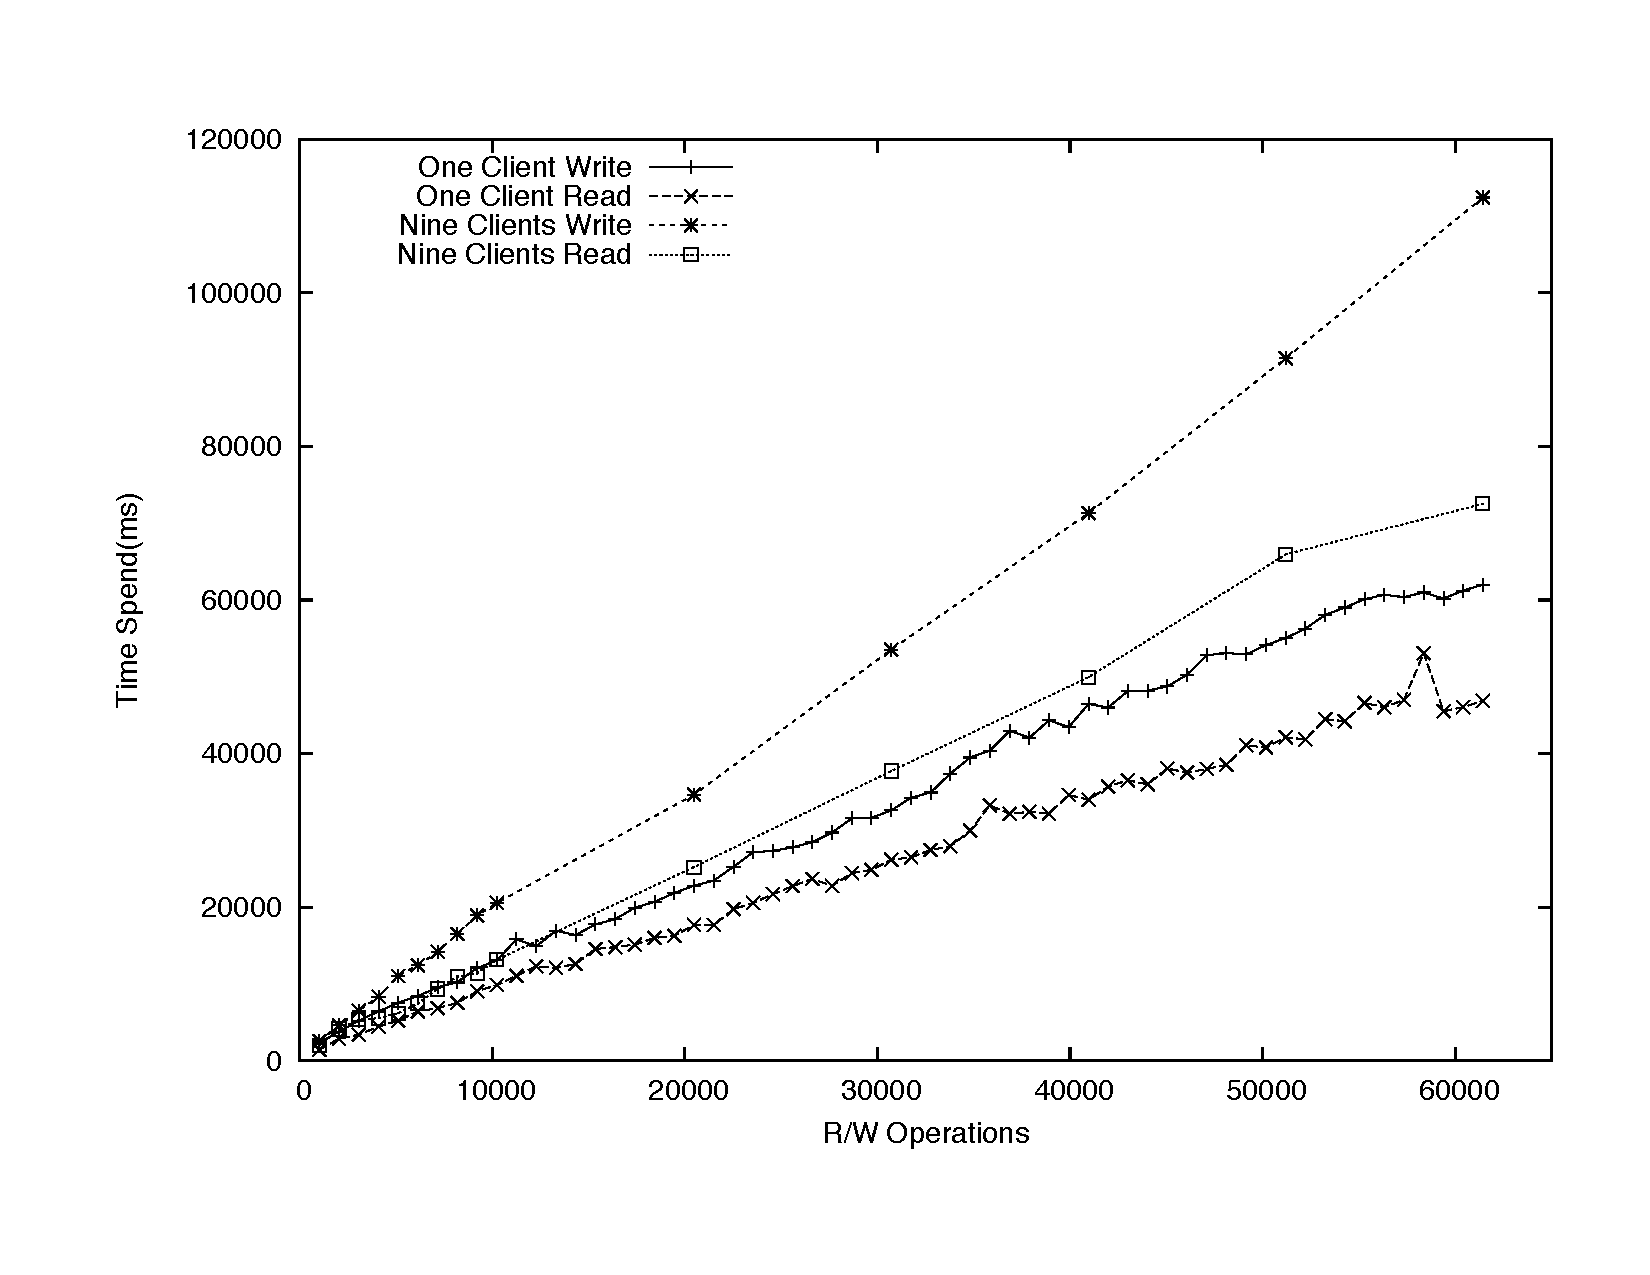
\includegraphics[width=5in]{../figures/sedna_one_client_nine_clients_compare.pdf}
\caption{多客户端和单客户端的读写性能对比(多客户端数据来自所有客户端的
  性能平均)}
\label{fig:perf}
\end{figure}

\subsection{ZooKeeper性能分析}

首先我们对本试验集群中运行的ZooKeeper集群进行一系列性能测试。从图
\ref{fig:zklatency}中可以看出一个同步的写操作在我们的集群中耗费了大约
10ms的时间,并且这个时间随着ZooKeeper节点的增加有所增加但是并不明显。
图\ref{fig:zkrlatency}展示了当ZooKeeper集群中节点数目增加时读延迟的变
化,我们可以看出当ZooKeeper读性能远远好于写性能。

\begin{figure}[h!]
\centering
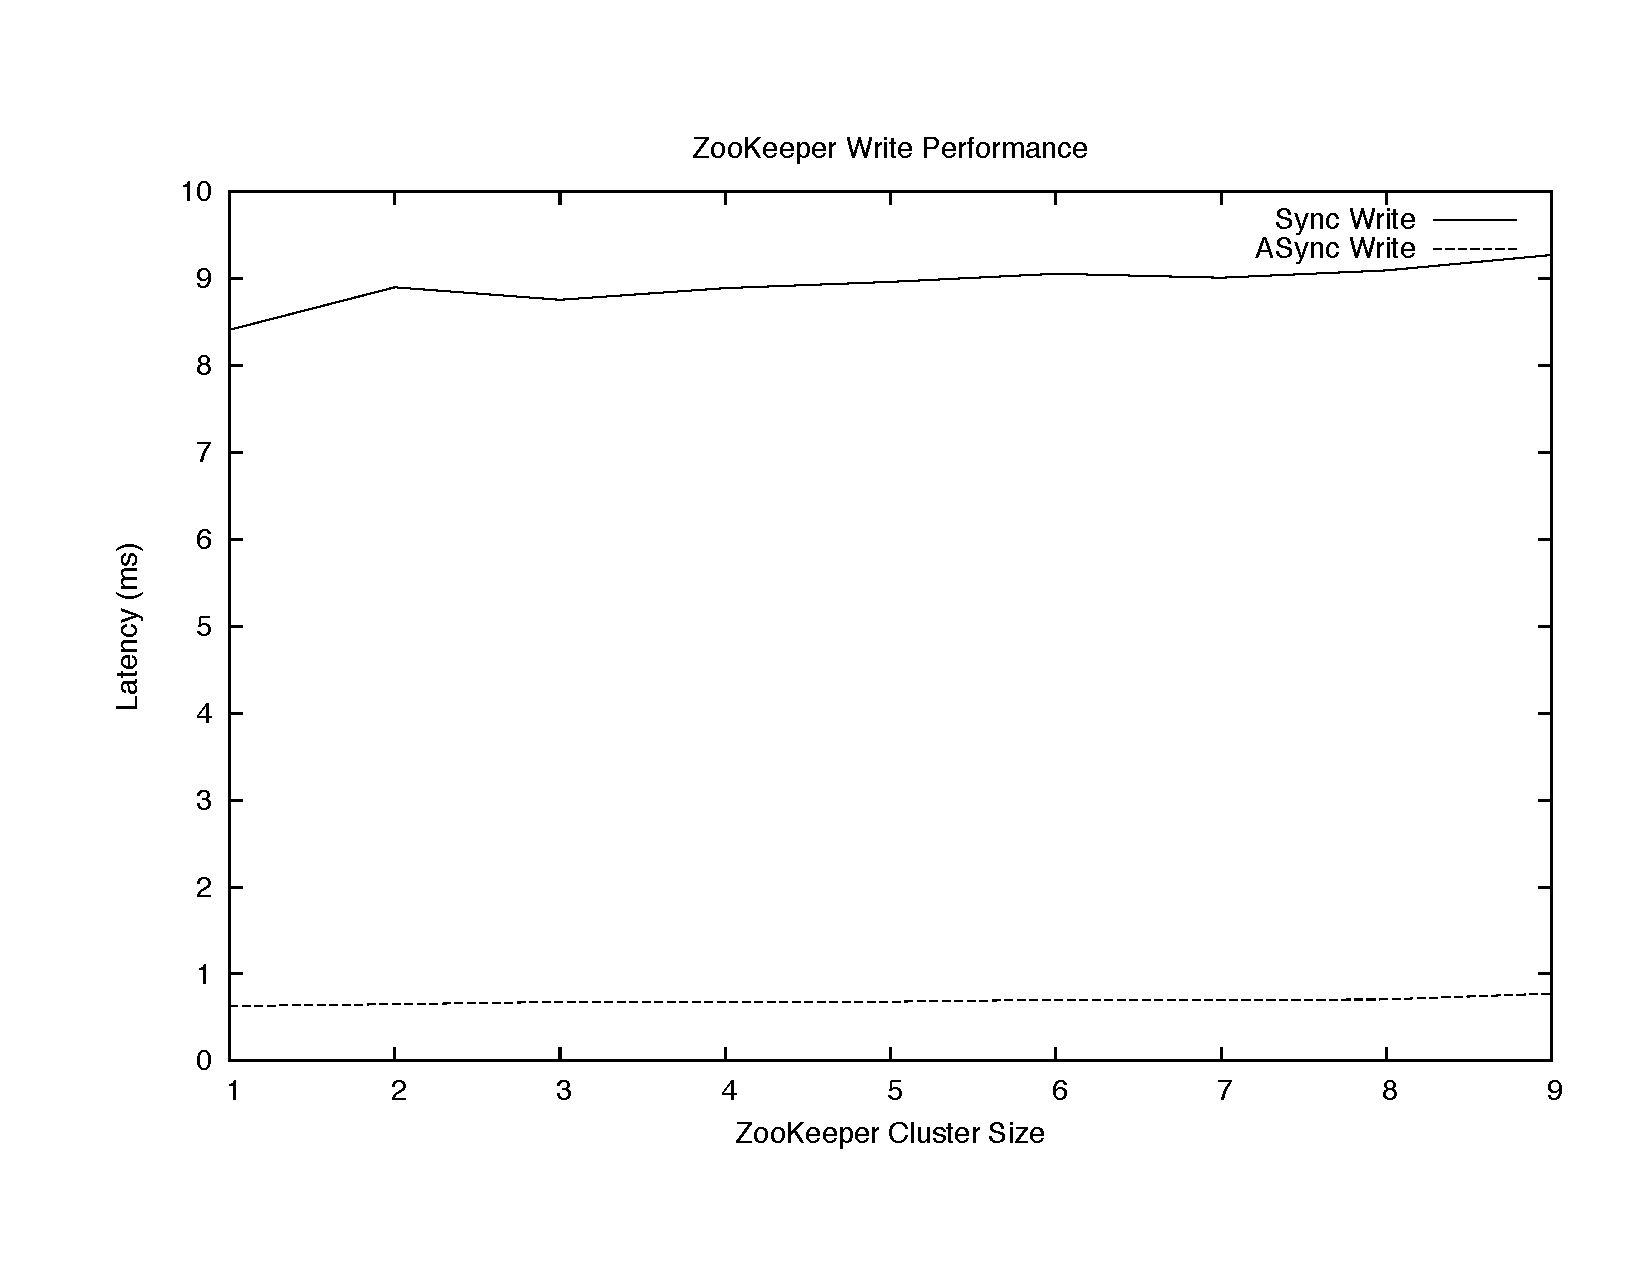
\includegraphics[width=4.5in]{../figures/zklatency.pdf}
\caption{ZooKeeper写延迟随着服务器数目的变化图}
\label{fig:zklatency}
\end{figure}

\begin{figure}[h!]
\centering
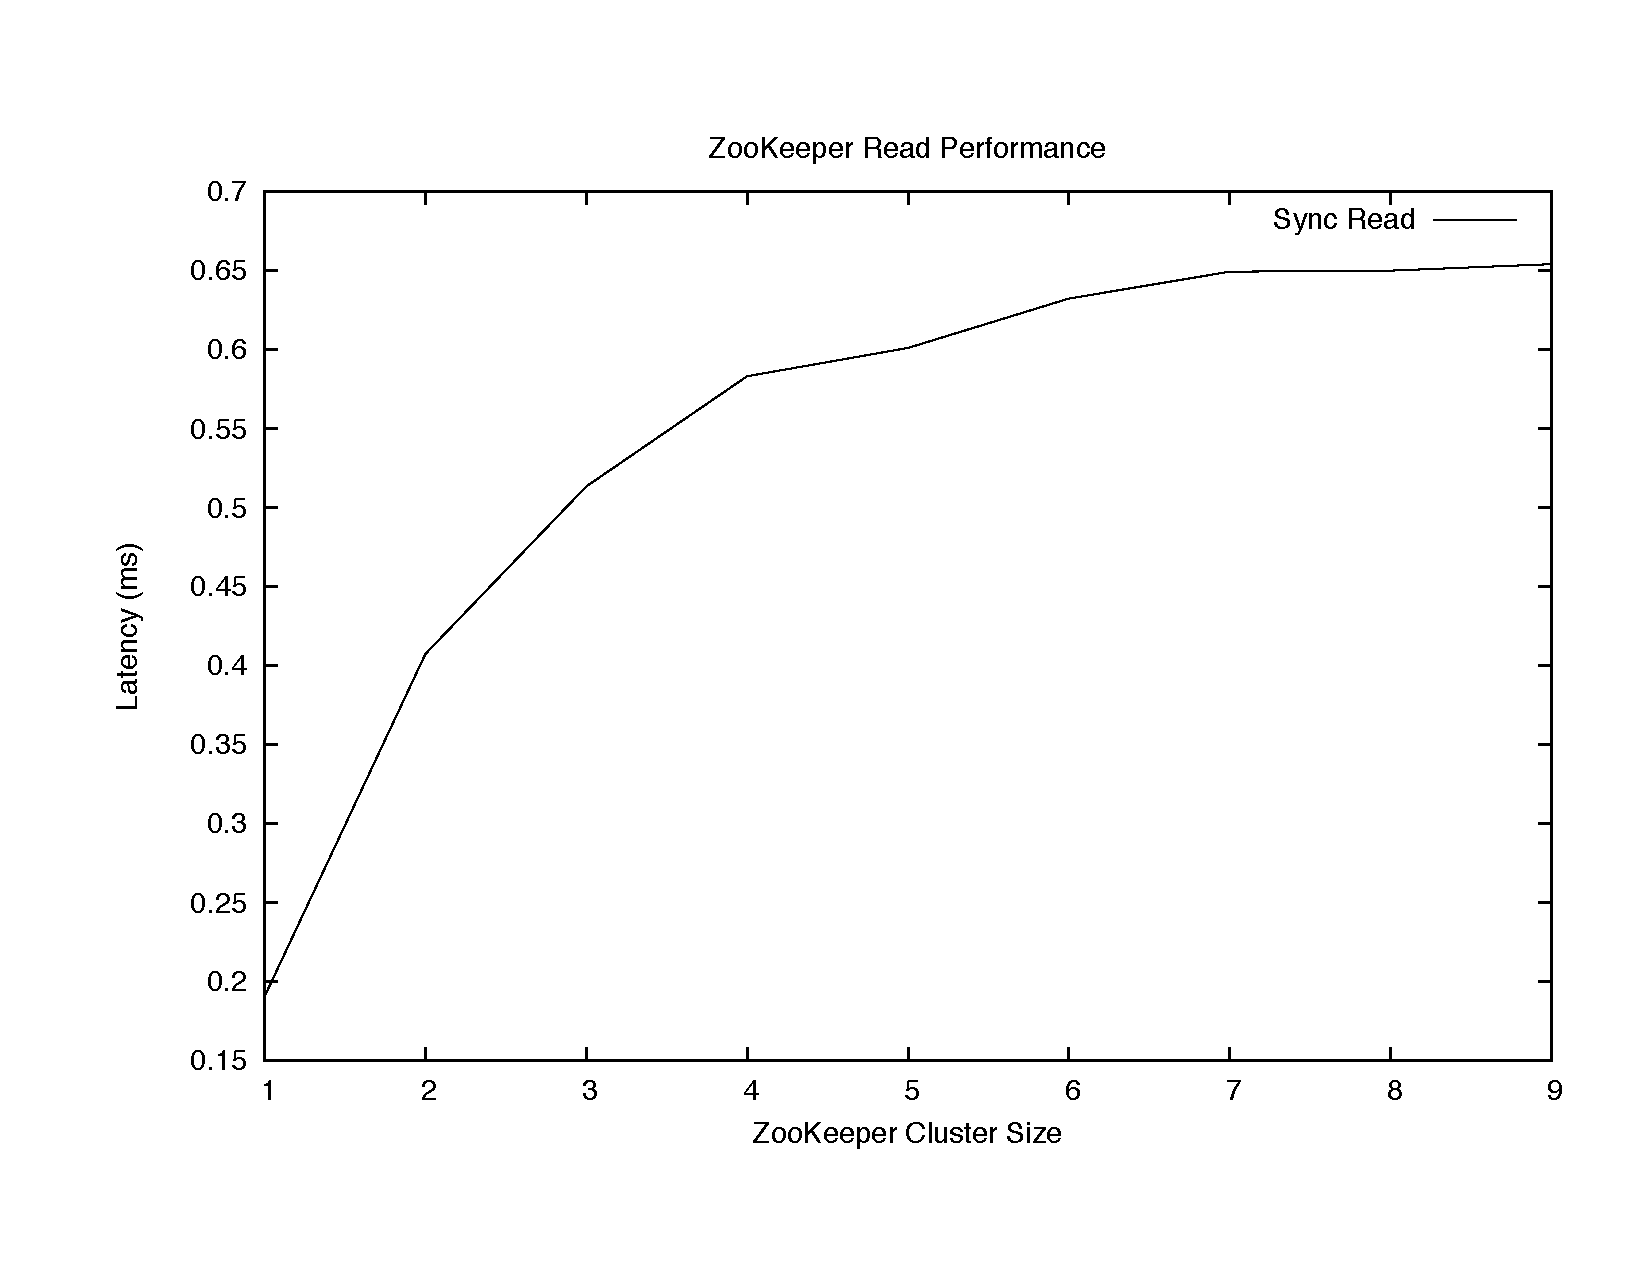
\includegraphics[width=4.5in]{../figures/zkrlatency.pdf}
\caption{ZooKeeper读延迟随着服务器数目的变化图}
\label{fig:zkrlatency}
\end{figure}

\begin{figure}[h!]
  \centering
  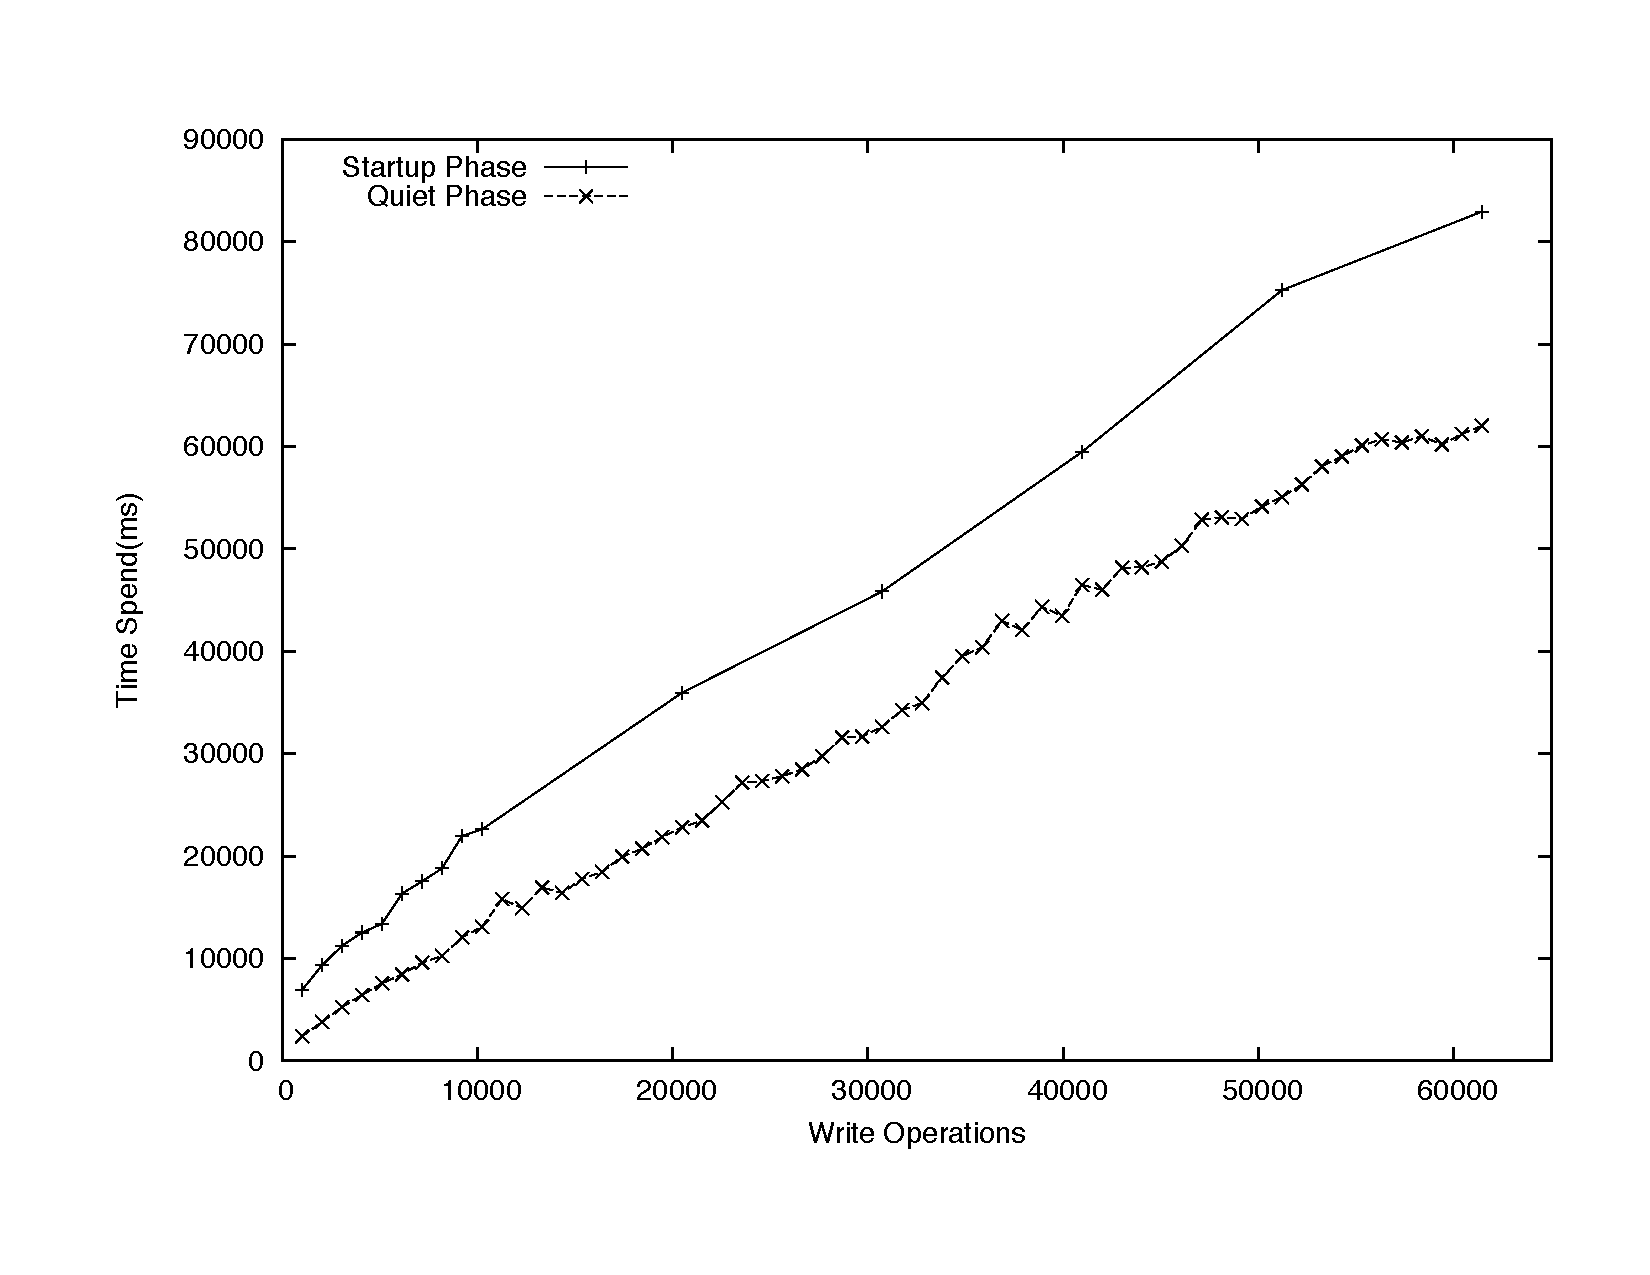
\includegraphics[width=4.5in]{../figures/sedna_write_quiet_startup_compare_one_client.pdf}
  \caption{启动模式和安静模式下单客户端性能对比图}
  \label{fig:zkquiet}
\end{figure}


为了证实ZooKeeper到底对Sedna系统性能的影响,我们在本实验中通过对启动阶
段性能和正常阶段的性能来比较。当Sedna集群第一次启动的时候,我们称这个
阶段为\textit{启动模式}。这个模式下,大部分的虚节点还没有指派给任何一个实节点,
此阶段需要进行虚节点的指派,需要非常频繁的写ZooKeeper。而这些写操作又
必须是顺序的,并且使得所有节点的本地缓存无效。这些动作会极大的降低
Sedna系统的性能。启动模式完成后,Sedna进入\textit{安静模型},在这个模式下,大
部分的虚节点都有了存储位置且相对稳定,且节点的缓存都是有效的,此时读写
性能达到峰值。通过观察这两个阶段的性能差别,我们可以看出最坏情况下,
ZooKeeper是如何影响Sedna系统性能的。从图\ref{fig:zkquiet}中可以看出,
这两个阶段的性能有一个比较明显的区别,不过两条曲线基本上保持了一个比例关系。

\section{小结}
\label{section:con3}
分布式存储系统作为云计算基础软件架构的核心对系统的性能起着至关重要的作用,为了支撑实时的云计算应用,我们设计并实现了一种完全基于内存的持久存储系统Sedna。Sedna能够在保证数据的持久性的前提下,为用户提供接近传统的内存缓存的性能。通过层次化的架构模型使得Sedna能够部署更多的服务器以提供与传统存储模型相同的存储容量。通过提供实时的API,我们进一步丰富了Sedna对实时应用的支持。通过对实时应用下存储系统的研究,我们认为使用内存作为优化只是解决了问题的一部分(提供了更快的数据的访问速度),而实际上我们面对的实时应用需要对数据的更新进行快速的反应,能够处理复杂的应用类型,这就需要计算模型的配合。因此,我们通过设计和实现一种基于触发器的通用编程模型来解决这个问题。

  \chapter{基于触发器的计算模型}
\label{chapter:domino}

\section{引言}

大数据时代的到来,人们每天搜集和存储的数据越来越多。这些数据中包含了各种有用的信息。比如电子商务网站会记录用户浏览历史,甚至浏览时鼠标停留的位置和时间。对每一个用户来说,这些记录的数据量并不大,但是对于通常拥有上亿用户的电子商务网站来说,记录这些数据就需要足够的资金来建立海量存储系统。企业愿意付出巨大成本来记录这些信息,是因为这些数据确实能为公司带来利润。利用这些数据对用户行为进行分析,能够非常准确的识别出每一个用户的特征、喜好、需求,并且针对性的给予商品推荐,从而提高推荐到购买的转化率。当然,除了存储处理这些本身就在赛博空间(Cyber Space)产生的数据之外,越来越多物理世界的数据也开始被数字化、收集并且加以利用,比如实时交通路况数据,街景信息,停车位信息,甚至是热门饭店的排位信息。在这些数据被存储之后,更重要的就是如何处理以利用他们。

大量像Amazon EC2或者Windows Azure等IaaS基础设施服务的出现使得按需获取大规模计算资源成为可能,这也使得利用这些海量的数据成为可能。然而,正如过去几十年计算机的发展所揭示的那样,设计和实现不同种类的可扩放的应用程序依旧非常困难,特别是对于需要大规模计算的领域专家而言,他们除了需要考虑应用本身的分布式实现之外,还需要考虑竞争条件、死锁、分布式状态管理、同步等非常复杂的技术问题。为了把应用开发人员和这些繁琐复杂的分布式问题分隔开来,大量的分布式计算模型开始出现。我们认为一个分布式的计算模型包括编程模型、运行时系统支持、容错恢复、任务调度、多用户管理等几个部分。

在现有云计算平台的多种计算模型的基础上,本章将介绍一种基于触发器的新型云计算平台中的计算模型——Domino。该计算模型包括了编程模型、运行时支持、以及容错恢复等部件,并且通过与现有的云计算存储系统整合,为开发人员提供了一个简单、直观、高效的大规模应用开发的计算模型。Domino通过整合HBase存储系统来为应用开发人员提供了完整的存储和处理基础设施以便用户更加容易的编写那些包含了大规模的迭代和递增处理的应用程序。

我们基于Domino模型实现了一系列示例应用,如PageRank、一些比较典型的机器学习和数据挖掘算法($K$-means, 协同过滤)、分布式的爬虫等。通过这些应用的编写和性能对比试验,我们认为Domino在递增计算场景下具备了比现有的云计算模型更为简单有效的处理能力。相比较传统的MapReduce以及其扩展模型,具有了更高的计算效率和简洁的编程抽象,更重要的是,Domino还为我们的大规模分布式应用程序提供了实时的容错恢复能力,这一点是现有的模型很难做到的。

本章将首先介绍现有的编程模型以及问题,详细的介绍基于触发器的编程模型。\ref{section:intro}节,我们将综合一个分布式爬虫的例子来介绍什么叫做\textit{基于触发器的}编程模型以及为什么使用触发器模型来进行编程;在\ref{section:sync}节,我们将着重介绍Domino中的同步模型;\ref{section:design}节具体的介绍Domino的实际设计与实现的细节;\ref{section:apps}节结合几个典型的应用介绍如何在Domino中实现不同种类的应用;最后在\ref{section:exp}节通过一系列的性能对比来验证Domino本身的性能以及其上运行的应用程序的性能。

\section{相关工作介绍}

\subsection{MapReduce模型及其问题}

MapReduce自从2006年由Google提出,之后由Apache基金会以Hadoop项目开源实现,当前已经成为云计算平台中的标准配置。作为一个批处理的计算模型,MapReduce非常适合于进行日志分析、离线推荐算法。然而MapReduce依旧存在很多问题:
\begin{enumerate}
\item 不能很好的支持小的任务或者交互式任务。来自Google的统计数据,一个MapReduce任务平均需要8分钟的时间来执行,而一个PageRank算法重新运行一轮甚至需要几天的时间。这导致现有的MapReduce十分不适合以下几种任务:实时搜索、在线推荐或者广告系统。可惜的是这些应用恰好是互联网收入的主要来源。再比如,在线推荐系统中,我们需要根据当前用户点击和浏览数据来计算新的推荐数据,这应该在几秒内实现。很明显的,现有的MapReduce是不符合的。

\item 不适合迭代式的数据处理。许多数据分析技术都需要交互式计算,包括新型的PageRank算法,HITS(Hypertext-Induced Topic Search),递归关系查询,神经网络分析,社交网络分析等。这些技术都有一个共同的特点:数据都是被迭代处理,直到计算收敛或者到达停止条件。MapReduce不能很好的支持这种迭代式的数据分析程序,开发人员只能通过编写驱动程序来手动的启动和管理多轮MapReduce工作。而这种开发方式显然不是一个好方法,1),每一轮迭代中,数据必须不断的重新载入,重新处理,这将极大的浪费I/O,网络带宽和CPU资源;2),停止条件或者收敛判断往往还需要一个额外的MapReduce来进行判断,这将引入非常大的延迟。

\item	MapReduce不适合进行数据源不断增加的分析任务。许多数据分析技术都需要对数据集进行递增计算,比如实时搜索引擎使用PageRank算法来对所有抓取到的页面排序,当爬虫爬取到部分新增网页,如果对所有页面一起运行完整的PageRank算法则极大的浪费了计算资源。可惜的是,这正是当前的实际情况。

\item 使用MapReduce的编程框架,应用程序不能在线访问计算的任何中间状态,只能通过将不同的数据流进行聚合来模拟传统的共享内存结构。

\end{enumerate}

为了解决这些问题,人们提出了许多改进和设计,我们将首先介绍其中的典型代表,并最终介绍基于触发器的计算模型。

\subsection{迭代处理模型}

HaLoop\cite{bu2010haloop}是一个基于Hadoop MapReduce模型针对迭代任务的改进版本。HaLoop不仅仅通过扩展MapReduce模型使其支持迭代应用,并且提出了迭代感知的调度器以及引入了迭代任务之间的缓存,极大的提高了迭代应用的执行效率。

\begin{figure}[h!]
\centering
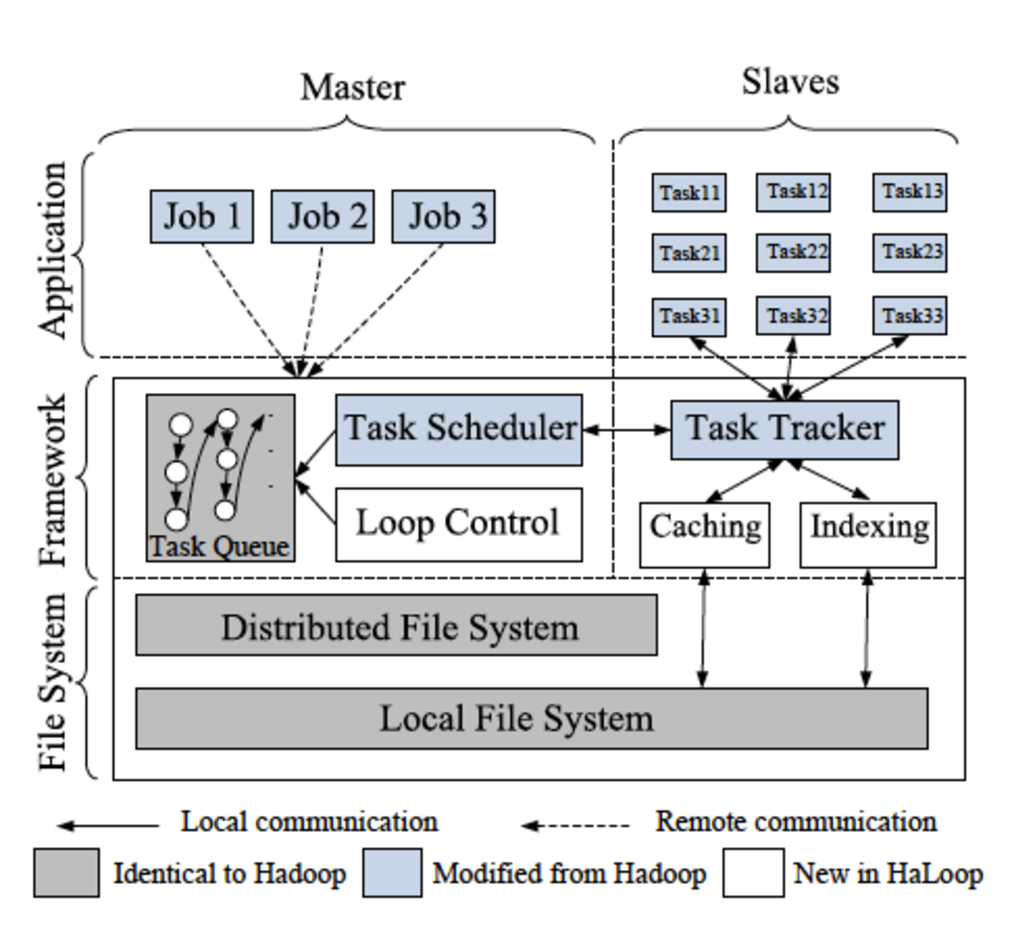
\includegraphics[width=4in]{../figures/haloop.pdf}
\caption{HaLoop架构图}
\label{fig:haloop}
\end{figure}

图\ref{fig:haloop}展示了HaLoop的整体架构。与Hadoop架构非常类似,HaLoop集群中包括了一个主节点和若干个从属节点。客户端向主节点提交任务,对每一个提交的任务,主节点会建立并且调度一系列子任务并发的在从属节点上执行。与Hadoop架构不同主要体现在,HaLoop的主节点包含了一个循环控制模块(Loop Control),能够不断的自动启动用户写入在循环体内的map-reduce任务直到用户指定的循环条件不再满足自动停止;其次,Haloop使用了新的任务调度器,该调度器能够感知到迭代计算的任务,并且通过将数据优先调度到数据所在的节点来提高数据的局部性。最后,HaLoop能够主动的在从属节点中缓存迭代过程中产生的不变量,同时也会缓存reduce的输出以加速下一个迭代的执行速率。

Haloop支持的迭代程序可以用下面的公式来描述:
\begin{equation}
R_{i+1}=R_0 \cup (R_i \bowtie L)
\end{equation}
其中$R_0$代表初始的结果,L代表计算过程中的不变量。

在HaLoop中编写程序时候,程序员应当指定循环体、循环终止条件以及循环不变量。为了帮助编程人员实现终止条件,Haloop提供了一些函数:\textit{SetFixedPointThreashold, ResultDistance, SetMaxNumOfIterations...}来提高编程效率。


Twister\cite{ekanayake2010twister}是另外一个支持迭代计算的MapReduce模型扩展。不同于Haloop,它使用了一种基于\textit{publish/subscribe}的消息传递的架构来进行数据传输和通讯以支持那些\textit{长时间运行}的mapreduce任务。

\begin{figure}[h!]
\centering
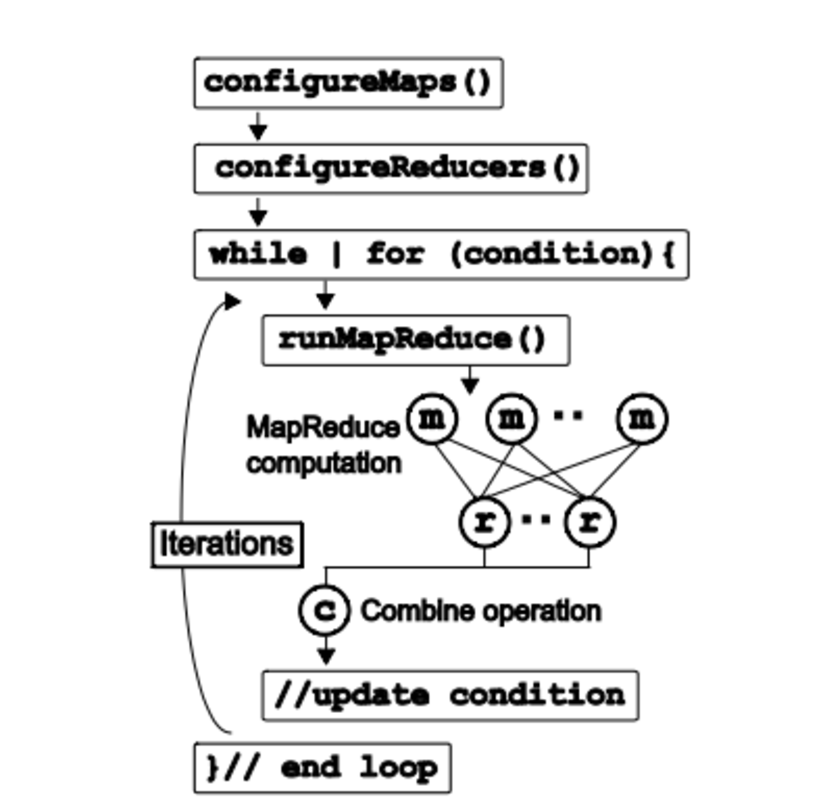
\includegraphics[width=3in]{../figures/twister.pdf}
\caption{Twister下迭代MapReduce编程模型示意图}
\label{fig:twister}
\end{figure}

图\ref{fig:twister}描述了Twister的扩展计算模型。Twister为MapReduce任务引入了配置阶段,在这个阶段里用户可以加载任何的静态数据以供后面的map和reduce阶段使用。那些长时间运行的mapreduce会将这些静态数据加载入内存以供迭代中不断使用。

图\ref{fig:twisterarch}进一步描述了Twister运行时的具体架构,其主要包括三个组件:1)客户端驱动程序,驱动了整个迭代程序的执行;2)所有的worker节点上运行的Twister守护进程;3)Broker网络节点。所有的worker节点启动后Twister守护进程会向Broker网络发起连接请求来接受命令和数据,该守护进程负责管理分配给自己的map和reduce任务,通知节点状态,并且最终需要对控制命令给予合适的响应。客户端驱动程序为用户提供了编程API并且将用户提交的API调用转变为控制命令和输入数据通过Broker网络发送给worker节点。

\begin{figure}[]
\centering
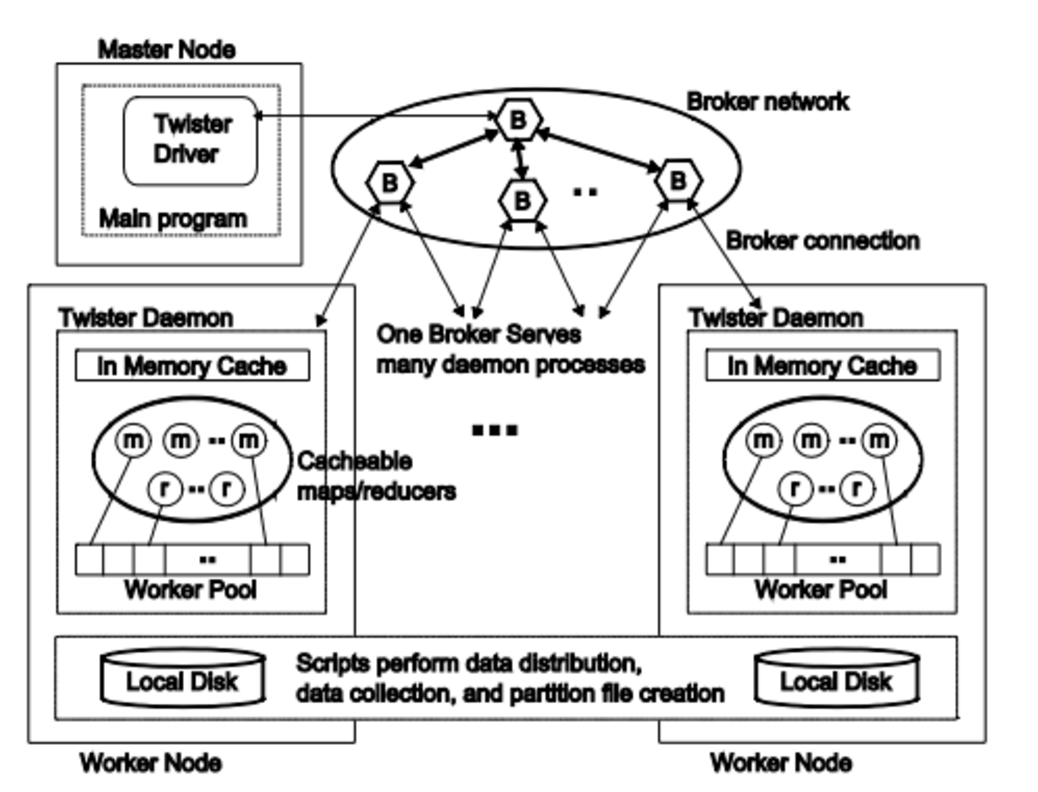
\includegraphics[width=4in]{../figures/twisterarch.pdf}
\caption{Twister系统的总体架构图}
\label{fig:twisterarch}
\end{figure}


\subsection{递增计算模型}

Incoop\cite{bhatotia2011incoop}是一个为了递增计算而修改的MapReduce模型,它不仅仅扩展了MapReduce,还结合了底层分布式文件系统,使得Incoop本身能够检测到输入数据的改变,并且通过一些细粒度的数据重用策略尽量避免不需要的计算,从而提高递增计算的效率。为了达到这个目的,Incoop对Hadoop系统做了几处修改:1)不再使用HDFS来存储输入数据和MapReduce任务的输出数据,Incoop基于一个修改版的Inc-HDFS来存储数据,其能够很好的识别出多次循环执行中输入数据中的相似部分;2)为了控制任务的粒度,尽可能的复用之前的计算结果,Incoop引入了一个新的Contraction阶段;3)Incoop提出了一个基于亲和性的调度算法,以减少task在多次执行过程中数据迁移。

Inc-HDFS改变了之前HDFS使用的基于固定大小进行分块的做法,转而使用基于内容的方式来进行分块。在Inc-HDFS中,引入了maker的概念,一个maker意味着一个特定的模式。当扫描输入数据进行分块的时候,如果当前所扫描的数据符合某一个maker,那么就将块边界定在此处。当然为了避免过大或者过小的块,其也设置了一些大小限制。

Incoop中的MapReduce任务执行至少有3个阶段:Map、Contraction、Reduce。所有的map都会将结果持久存储以来,并且把存放的位置信息和map任务的相关信息存放在单独的备忘服务器中,以供日后重复使用。为了减少Reduce任务的粒度,引入了Contraction阶段。Contraction是基于原MapReduce中的combiner实现的。Contraction阶段的结果可以被更好的重用。

Incoop引入了基于备忘服务器的亲和性调度算法。它试图在尽量提高局部性和减少straggler之间取得平衡。该调度算法为每一个物理节点维护一个单独的任务队列,每一个任务队列都包含了根据备忘服务器的数据而最应该在本节点执行的任务集合。每次取任务都从本节点的任务队列中优先取出,直到为空,方从别的节点“偷取”任务执行。

Percolator\cite{peng2010large}是由Google于2010年提出的一种事件驱动的处理模型,专用于递增计算。Percolator在Google内部被广泛应用于实时搜索引擎业务。通过实际使用,Percolator相比MapReduce方案可以提供相同的数据处理量,而将数据处理的更小效率提高了一倍。

Percolator是专为搜索引擎而设计的。如果爬虫爬取了一部分新的互联网页面,如何处理并且建立索引呢?仅仅因为这一些新数据就重新运行一个完整的MapReduce任务是不合适的,效率太低了,因此递增计算是一个较好的解决方案。Percolator提供了对多达几个PB的数据集的随机访问能力,ACID的事务机制。为了帮助程序员来追踪递增计算的状态,它还提供了观察者机制:一段用来观察指定的数据域改变从而触发执行的代码。一个典型的Percolator程序就是一系列观察者的序列,每一个观察者都可以通过修改数据从而触发下一个观察者。

Percolator最主要的贡献在于它提供了两个非常重要的实现来支持递增计算:分布式事务以及通知机制。在一个可以随机存取的存储系统之上提供ACID事务是非常困难的,而且该事务是跨行的、跨表的。为了提高效率,Percolator中的事务是通过独立快照实现的,他不能提供串行读写保证,但是却更高效。 Percolator主要是通过Bigtable来实现包括独立快照、读写锁等机制的。锁信息存放在Bigtable的某一列中,为了处理由于节点失效可能导致的死锁,Percolator又引入了主锁的概念。通知机制也是Percolator的一个创新,其中的观察者作为Percolator的基本单元以组成一个应用程序。每一个观察者都会完成一个任务并且通知下一个观察者来执行。该通知机制有点类似于数据库中的触发器,但职责不同。Percolator的观察者实现具有几个优化的地方,首先保证多次触发同一个观察者不会导致任务重复执行;其次提供了一个非常有效的方法来寻找表中改变的项目。


\subsection{实时处理模型}
随着Web 2.0站点和移动互联网的兴起,用户开始尝试在互联网上共享更多的数据,而且这些数据的生命期也变得越来越短。对用户提交的新数据进行快速的分析需要能够进行实时计算的编程方法。当然,实时计算的范围相比迭代计算和递增计算可能更宽一点,它有可能包括这两种计算模式中的一部分,然而,实时计算最基本的特点是其对计算时间和计算延迟的关注。

论文\textit{Analytics for the Real Time Web}\cite{grinev2011analytics}中提到了一种扩展已有的Key-Value存储架构以提供实时计算模型的方法。该论文扩展了Cassandra存储系统,加以基于推送的处理协议,增加了对任务执行事务性的特点。总体上来说还是一种基于MapReduce风格的计算模型,不同的是其修改了Reduce函数,变为Reduce*函数。该函数能够递增的接受来数据输入,这也意味着用户可以不断的将数据推送给Reduce*函数,而须一定按照MapReduce框架所规定的那样,只能由Map或者Combiner函数来发送数据。唯一的局限在于并非所有的Reduce函数都可以转化为可以递增计算的Reduce*函数。

\begin{figure}[h!]
\centering
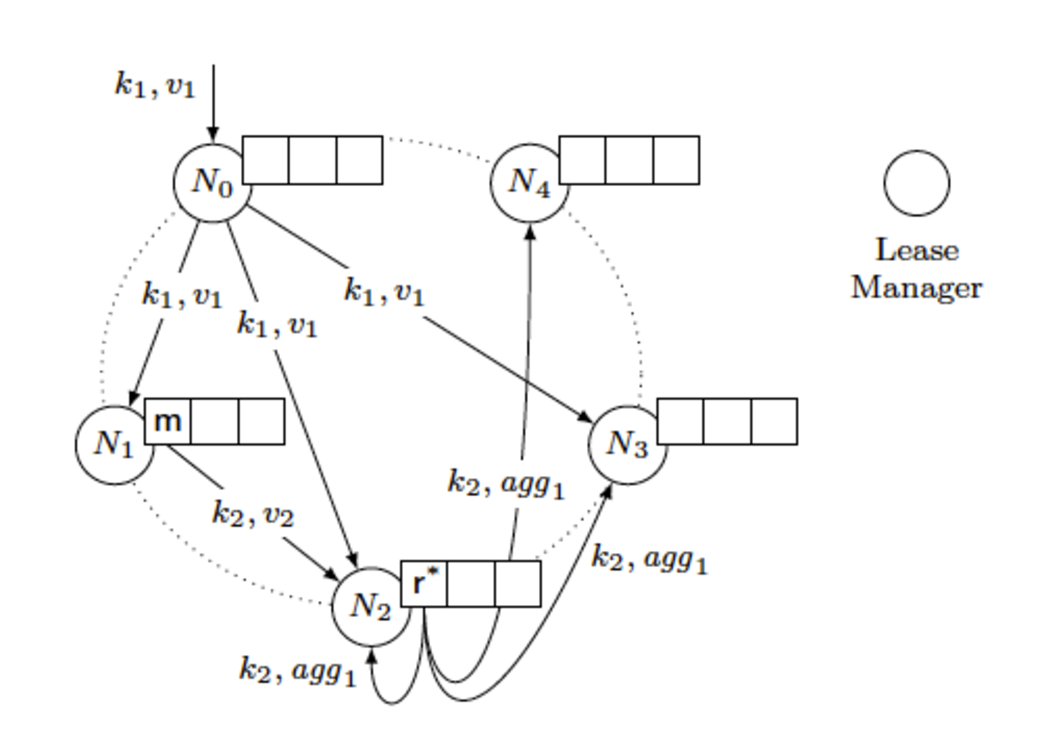
\includegraphics[width=4in]{../figures/realtimep.pdf}
\caption{实时MapReduce模型下map/reduce*的执行流程}
\label{fig:realtimep}
\end{figure}

图\ref{fig:realtimep}展示了一个如何利用本系统进行实时计算的流程。每当一个key-value对被插入到Cassandra系统中的时候,该节点就会执行一个分布式的事务:1)复制该key-value到多个节点;2)选择一个备份节点作为执行map程序的协调者;3)将map任务放入本地的任务队列中。而map任务的执行也是一个分布式的事务:1)将任务从队列中移除;2)将map输出写入到对应的reduce*节点;3)将reduce*任务放入到本地任务队列。而map输出将相同的key值路由到相同的节点中,reduce*的输出会将结果保存到多个节点中。事实上reduce*的执行过程也被视作一个分布式的事务,包括将数据写入多个节点中,以及将reduce*任务正确的从任务队列中移除。

\subsection{前人工作的不足及新的方案}

虽然上一节我们已经简单的介绍了很多分布式计算模型,然而实际上单纯列举已有的分布式计算模型就远远超过了本文的篇幅,我们在这里按照数据访问的模型对他们进行一个简单的分类并且分别讨论他们的缺点和不足。

上面我们所描述的编程模型中很大一部分是同步的数据流模型,这些模型针对的是那些面向数据流,并且对数据流进行同步的多轮处理的应用程序。比较典型的代表如MapReduce\cite{dean2008mapreduce}以及Dryad\cite{isard2007dryad}模型,以及一些基于它们的扩展模型\cite{bu2010haloop,ekanayake2010twister,zhang2011priter}。这些模型非常适合处理那些不需要访问全局共享状态的批处理应用,像\textit{wordcount}或者\textit{sorting}能够被很容易的在该模型下实现,这其中的一些扩展模型能够处理迭代计算,不过MapReduce模型本身的数据流模型使得访问计算中间状态变得非常复杂,这个限制使得这类编程模型在复杂的迭代计算场景下还是显得无能为力。

一些编程模型提供了面向数据的模型,比如Piccolo\cite{power2010piccolo}以及Pregel\cite{malewicz2010pregel},这些模型提供面向对象的数据访问语义,允许用户直接访问任意的数据而不须将数据抽象为数据流来处理。由于没有数据流的概念,为了保证并发执行时数据的一致,该类模型需要引入全局屏障(global barrier)以同步程序的执行。同步的计算模型抽象虽然简单,但是却会极大的提高程序的执行时间,因为每一个阶段的执行时间都是由最慢的执行所决定。

与同步面向数据的模型相对应的是提供了异步语义的面向数据的编程模型,比如Oolong\cite{mitchell2012oolong}以及GraphLab\cite{Low:2012:DGF:2212351.2212354}等,其中GraphLab是一个针对图应用设计的编程模型,用户需要将其需要解决的问题抽象成为图算法来解决,这在某种程度上也限制了其应用范围。

Oolong和Percolator同属于递增编程模型,它们针对递增处理应用而设计,从模型的角度来说很好的解决了递增计算和迭代计算对模型的需求,然而却在同步和错误处理上存在较大的问题。对于数据同步,Percolator选择使用分布式事务来管理程序执行的状态,Oolong则是通过用户提交的聚合函数作为全局屏障来同步程序的执行。Percolator的问题在于大量的事务和锁非常容易使得开发人员写出效率低下的分布式代码;而Oolong使用的聚合函数过于简单,对于稍微复杂的同步需求就无能为力,这类面向递增处理应用而设计的编程模型太过简单,并且非常有针对性,无法作为一种通用的编程模型出现。

面对这些编程模型的问题,我们提出了一种基于触发器的通用编程模型并且基于该模型设计和实现了运行时系统,统称为Domino计算模型。该模型特别适用与对时间要求较高的迭代和递增应用,亦可作为一种通用模型用于多种应用中。该计算模型具备以下几点创新性:

\begin{enumerate}
\item 完善了触发器的基本概念,在分布式环境下提出了将触发器作为通用的基本编程模型的思路和设计方案,能够用于不同的应用程序。

\item 提出了聚合模式对触发器的执行进行聚合,通过引入三种不同的同步模型:完全异步、最终同步、严格同步来支持同步及异步的应用。

\item 提出并实现了一种基于触发器的编程模型上的实时的容错恢复策略,能够有效的降低由于节点失效带来的应用处理速度延迟。
\end{enumerate}

一个典型的Domino的应用是通过组合一系列的触发器实现的。每一个触发器都是由用户编写的代码块组成,并且在特定的事件发生的时候被触发执行。比如在一个电子商务网站中,系统需要根据用户的购买历史和点击评分推荐其最感兴趣的商品,为每一个用户计算推荐商品的过程通常是若干个机器学习算法的组合。由于需要处理的数据量较大,且每一次完整的计算过程复杂度较高,因此通常需要在后台离线的计算,从而无法根据用户当前点击的情况为其推荐商品。然而用户当前的点击情况恰恰最精确和及时的反应了他的购买兴趣。然而使用触发器模型编写的推荐算法,可以通过监测用户点击事件来执行。执行过程中只需要对发生改变的部分数据进行重新计算,从而极大的降低了计算复杂度,能够实时的给出准确的推荐结果。

触发器模型虽然在此类在线复杂应用中效果较好,但是作为一种通用的编程模型却存在一些重要的挑战。这些挑战包括下列两点,我们在后面的Domino系统的设计和实现中将描述这两个挑战是如何在Domino中得到解决的。

\begin{enumerate}
\item 计算的同步问题。触发器模型的动作执行原生上是完全异步的,没有有效的同步控制方法,但是同步多个并行的计算流程却是分布式应用最基本的需求。比如MapReduce应用的Map和Reduce阶段直接天然的形成了同步语义,而MPI/OpenMP等应用中也需要用户显式的插入同步原语来保证不同执行语义的同步。

触发器模型无法简单的套用这类方法,原因如下。假设用户提交触发器$tr$以监测数据集$D_s$,当$D_s$中数据发生改变的时候,在不同服务器上的$tr$就会执行,并且产生需要同步聚合的中间结果。若该触发器程序处理的输入集是不断变化的(递增计算中较常见),那么系统在某一时刻有多少个$tr$会执行是是不可知的,该数目仅仅与当前输入数据集的改变有关。这也就导致我们无法在同步点准确的知道需要等待多少个$tr$的执行结果,因此无法有效的判断同步返回时刻。如果Domino应用不需要处理变化中的数据集,这个问题就可以通过使用传统的同步原语比较简单的解决。

\item 触发器模型将一个大规模的计算任务划分成针对数据改变的小的并发任务。这些并发任务的粒度较小,且并发的运行在大量的服务器中。这引入的一个大问题就是如何对节点的崩溃和任务的异常进行检测、恢复。

由于基于触发器模型的应用程序多需要处理不断流入的数据流并且较快的给出结果,如果触发器的某些节点上的实例由于节点失效而无法处理,就需要快速的恢复策略,而不能像MapReduce模型那样重新提交任务执行。为了支持实时的应用,须在触发器模型上实现更为有效的容错和恢复策略。

\end{enumerate}

\section{基于触发器的编程模型}
\label{section:intro}
\subsection{触发器模型}
触发器的概念在计算机科学中出现已经超过30年了,因为在很多传统系统中,组件需要对刚刚更新的对象进行识别并且针对性的执行一系列的操作。普遍认为这种方式能够提供更好的软件模块化能力,因为更新模块和处理该更新的模块可以独立起来。比如,一个雷达物体扫描程序会不断的更新敌军飞行器的位置,那么我们系统中应该同时有一个基于敌机出现或者位置改变发射火箭进行摧毁的模块来响应雷达扫描程序的输出。通常有两种做法来完成此类工作:一种是该模块不断的检查(\textit{轮询})感兴趣的对象,并且当发现对象发生改变时执行特定的动作。此方案最大的缺陷就是浪费资源,并且响应时间完全受限与轮询的时间间隔,而若设置较小的时间间隔,会浪费更多的资源。另外一种则是模块在某处等待直到感兴趣的对象发生改变才被激活执行特定的动作,我们也称之为触发模型。

从上个世纪90年代起,数据库领域出现了研究主动数据库(Active database\cite{rabuzin2007theory,mccarthy1989architecture, jaeger1999parallel, gehani1991ode,dayal1988hipac,chakravarthy1994composite})的热潮,主动数据库就核心概念就是利用触发器实现的一种面向数据的主动执行的概念。在主动数据库中,数据库操作或者外部的事件在满足一定条件的基础之下都能够触发特定动作执行。从概念上来说,主动数据库中的执行流程满足ECA规则,ECA即Event-Condition-Action。当一个事件发生的时候(On Event),并且特定的条件被满足了(IF CONDITION),然而指定的动作就将被执行(THEN ACTION)。主动数据库后来被广泛实现于商用数据库系统中(一般都是通过触发器或者触发器过程来实现),比如Postgres\cite{stonebraker1988postgres},HiPAC\cite{dayal1988hipac},Sybase\cite{darnovsky1987transact},VBase\cite{andrews1987combining}以及OOPS\cite{schlageter1988oops}等。然而直到今天,我们可以发现,虽然在理论上已经有很多关于ECA规则的研究,然而作为主动数据库理论核心的触发器依然是作为一个保持数据一致性、完整性或者安全检查的辅助工具存在于数据库中,没有成为通用的编程模型,其中主要原因是数据库由于需要支持ACID属性,使得触发器的实现复杂度太高:虽然相比较传统的面向程序的编程模型,基于触发器的编程模型能够在触发器数目较小的情况下提供明显的响应速度提升,并且通过将较大的应用分解成为一个个小的触发器来模块化应用并加以管理,不过,由于触发器对数据库领域最为核心的ACID特性,特别是事务机制的挑战,使得触发器的执行效率非常低。

不过情况在分布式环境下开始发生变化。根据之前介绍的CAP所描述,在一个分布式的系统无法同时提供一致性、可用性以及分割容忍三个特性。而且现有的云环境中,我们更加重视可用性和分割容忍性,因此一致性往往成为我们牺牲的选择。在新的NoSQL或者NewSQL的分布式存储系统中,人们尝试提供最终一致或者仅仅单节点内的原子性等。在这种情况下,分布式环境下,触发器模型也逐渐成为一个好的选择。

\subsection{Domino的编程模型}
Domino严格遵守了ECA模型,它将一个用户程序抽象为:事件监控(Event)、条件判断(Condition)、以及动作(Action)执行三个部分。为了更清楚的展示如何使用Domino模型来编写应用程序的,我们这里使用一个简单的分布式爬虫作为例子来介绍。

\begin{quotation}
\textbf{[分布式爬虫实例]}最基本的分布式网页爬虫非常简单,它开始于几个简单的网页URL地址,不断的将这些网页读取下来并且进行分析,通过分析网页的外链,爬虫将会获得更多的网页URL地址,周而复始直到爬取到某种限额或者整个网络。当然,一个可以工作的网络爬虫不止这么简单,它需要遵守Robots协议,需要考虑到网络带宽,需要考虑页面更新等等。而在我们的这个简单的例子中,我们并不会把重心放在这些功能上,而是更加关注网络爬虫的核心功能:爬取页面,分析页面。

本文实现的爬虫并不爬取互联网上的通用网站,而是爬取一个新型的社交网络上的信息(新浪微博)。微博是一种新型的社交媒体,所有的用户都可以发表公开的不超过140字的消息并且评论、转发他人的消息。由于其简单且交互性强而非常活跃。由于其时效性强,我们希望爬取能够爬取最新的消息,并且希望我们的爬虫可以以更高的优先级爬取那些\textit{更重要}的消息。这里的\textit{更重要}使用评论数加转发数的方式来定义,如果一个消息的评论数和转发数更多,那么它就更加重要。

基于Domino实现的网络爬虫程序的过程主要包括两部分,首先通过编写触发器监控存放微博信息的表,当用户有微博更新的时候,触发动作执行来获取该微博所有的评论或者转发的用户。这些用户我们称为\textit{当前活跃用户},并且记录下来。每次发现新的当前活跃用户,另外一个触发器就会执行,尝试抓取这些\textit{当前活跃用户}最近的微博消息,写入存放微博信息的表中,写入成功就会再次触发第一个触发器执行,以次往复,爬取微博消息。具体来说,触发器\textit{WBContentTrigger}负责监控微博消息表,当其中出现新的微博的时,获取该微博的所有评论或者转发的用户的信息,写入到微博用户信息表中;触发器\text{WBUserTrigger}负责监控微博用户信息表,当该表中某一个用户状态发生改变,意味着最近该用户曾经评论或者转发过别的用户信心的时候,该触发器将负责爬取这个用户最近的微博消息,并且写入到微博消息表中。
\end{quotation}

\subsubsection{事件(Event)}
触发器模型中,首要的元素就是ECA中的Event即事件。事件的种类非常多,按照之前在主动数据库中的分类,事件一般可以被划分为简单事件和复杂事件。其中简单事件主要包括了:时间事件(包括绝对时间事件和相对时间事件),方法事件(比如某个方法被调用而产生的事件),事务事件(比如事务提交或者准备事件),以及数据事件(比如数据被读取或者写入产生的事件)等。而复杂事件则是简单事件的组合或者是使用简单事件加上某些特定语义来组合,比如在某一个时间周期内未出现某个事件就被认为是一个复杂事件等等。然而在Domino中,我们主要关注的应用场景就是希望对存储在系统中的数据变化进行监控,因此我们主要提供了数据事件,特别是写数据事件的实现。当然时间事件也是很应用很广泛的事件源,不过由于分布式场景下时间的不一致导致我们无法给出一个用户一个统一的准确的时间线。由于时间的不统一,使得可用的时间事件粒度较粗,比如每个一个小时、每隔一天。对于这种应用,我们可以很简单的将时间事件委派给周期任务去执行,而不是通过Domino来实现。因此,Domino中主要关注了数据写事件。

\begin{figure}[h!]
\centering
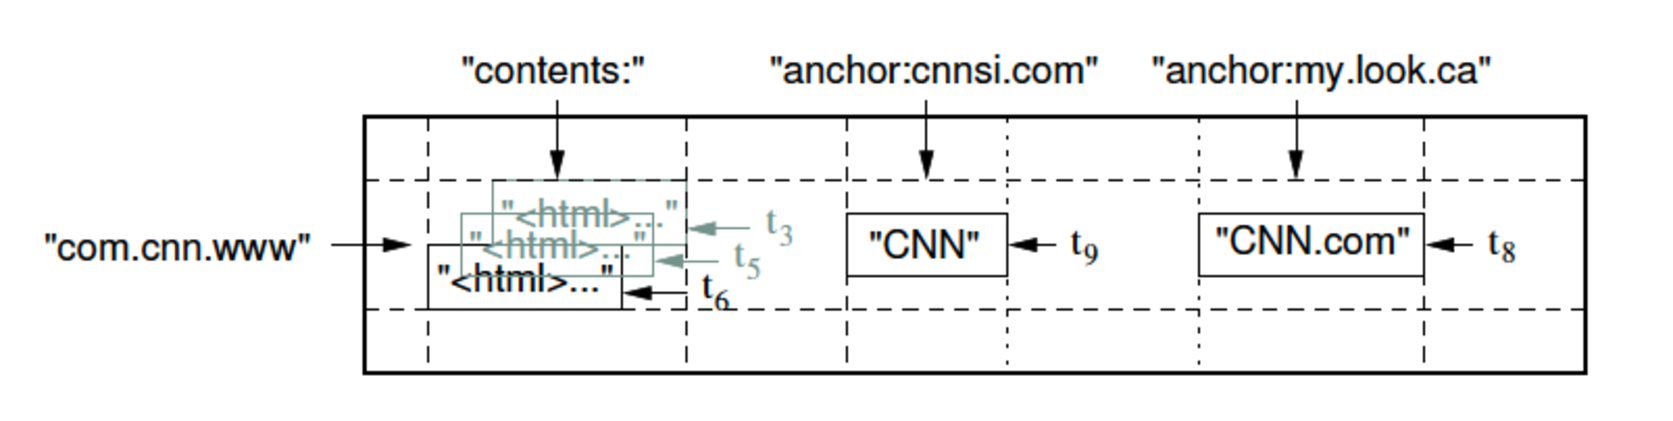
\includegraphics[width=4in]{../figures/bigtable.pdf}
\caption{HBase的基本数据单位:表的组成}
\label{fig:hbase}
\end{figure}

数据写事件来源于外界或者触发器本身对底层存储系统的写动作。当前版本的Domino是基于HBase实现的,因此我们首先对HBase中存储的数据结构进行一个简单的介绍。在HBase\cite{chang2008bigtable}中,数据是以表为单位存储的。表中的元素通过使用行关键字来区分,每一个行关键字都可以是任意一个字节串,而且HBase保证了所有针对字节串的读写都是原子的。如图\ref{fig:hbase}所示,HBase中的每一个表通常包含了数以亿行的数据,每一个行最多可以存储上千个列族以及上百万个列。列是以列族的方式组织起来的,每一个列族中可能包含不定数目的列,这些列可以在程序运行的过程中随时增加,列族也是进行访问控制的最小单元。每一个行列定位一个cell,其中存储着多个版本的数据。数据版本是一个64bit的整数。在cell中所有数据按照数据版本顺序以堆栈的方式堆叠起来。HBase中,如果想要使用某一个列族,开发人员必须事先新建该列族,或者通过改变表的属性来增加列族,列族被创建之后列才能被使用,用户通过指定\textit{列族:列}来制定一个cell。前面提到了Domino是通过修改HBase来实现的,在Domino中,我们要求用户提交触发器的时候指定所要监控的事件,默认情况下就是数据更新事件。这个事件中必须制定所监测的表、列族,列则是可选的,如果不指定列,那么所有该列族中的列上的更改都会产生数据更新事件。



\begin{table}[hb]\small
	\begin{minipage}[t]{0.5\linewidth}
	\centering
	\caption{HBase中表\textit{WBContent}的结构}
	\label{table:wbcontent}
	\begin{tabular}{|c|c|c|}
		\hline
		\textit{MessageId} & \textit{Content:zh} & ...,... \\
		\hline
		\textit{Message-1} & $content_{1}$ & ...,... \\
		\hline
		\textit{Message-2} & $content_{2}$ & ...,... \\
		\hline
		... & ... & ...\\
		\hline
	\end{tabular}
	\end{minipage}
	\begin{minipage}[t]{0.5\linewidth}
	\caption{HBase中表\textit{WBUser}的结构}
	\label{table:wbuser}
	\centering
		\begin{tabular}{|c|c|c|}
			\hline
			\textit{User Id} & \textit{Activity:recently} & ...,... \\
			\hline
			\textit{User-1} & $true$ & ...,... \\
			\hline
			\textit{User-2} & $true$ & ...,... \\
			\hline
			... & ... & ...,...\\
			\hline
		\end{tabular}
	\end{minipage}
\end{table}

\begin{quotation}
\textbf{[分布式爬虫实例]}在Domino网络爬虫的实现中,我们需要监控两个数据写事件。一个来自由于爬取到新的微博数据而修改的WBContent表的列: \textit{Content:zh},另一个来自于由于猜测到某些用户可能最近更新了微博页面的WBUser表的列:\textit{Activity:recently}. (触发器WBContentTrigger所监控的表如\ref{table:wbcontent}所示,而触发器WBUserTrigger所监控的表如\ref{table:wbuser}所示)。
\end{quotation}


\subsubsection{条件(Condition)}
触发器模型中,条件是一组用户自定义的函数。该函数的传入参数是封装好的事件,返回值为true或false来表明当前用户制定的条件是否满足。在Domino中,条件(condition)包括了三种,分别负责三个关键的功能:首先,由于触发器一旦提交到系统中就会持久存在除非用户显式的取消该,但是在大多数情况下,我们希望触发器能够在到达某些条件的时候自动停止,而不是永远运行。在这种情况下,用户就可以通过编写停止条件(stop condition)来实现判断。除此之外,由于Domino中的事件都是由数据写入引起的,如果短期内写入频率非常高,对它们进行快速处理就会极大的占据系统资源,在这种情况下,用户就可以通过编写间隔条件(interval condition)来为每一个触发器指定执行的周期。其实在Domino中,每一个活跃的触发器都是有一个最大执行频率的,用户可以通过编写条件函数覆盖该设置以加入自己的频率控制语句。最后,Domino还引入了选择条件(select condition)来对事件进行选择,仅仅处理其中一部分事件,该条件对于很多高效应用非常重要。

停止条件(stop condition)中非常的应用在那些迭代收敛的应用中。比如PageRank或者很多机器学习算法,这些算法中,往往需要判断连续两次迭代中计算的值之差是否足够小。如果足够小,程序就可以停止运行。Domino对这种应用做了特别的优化,每一个传入条件函数的封装好的事件都包括了更新前的值和更新后的值。

\begin{quotation}
\textbf{[分布式爬虫实例]}对于爬虫来说,我们不需要特别的停止语句,因此我们将默认使用Domino本身提供的条件函数(如\ref{code:wbcrawler}的filter函数所示),实际Java代码实例如下:
\begin{lstlisting}[language=java]
  //过滤器,用来判断这个事件是否应该使触发器执行。这里永远返回true
  @Override
  public boolean filter(HTriggerEvent hte) {
    return true;
  }
\end{lstlisting}
\end{quotation}

\subsubsection{动作(Action)}
触发器模型中,动作函数(Action)是由用户编写的一段代码块来执行所需要的代码逻辑。Domino为用户的动作函数提供了完整的变量封装以提高用户代码执行的效率,如\ref{code:wbcrawler}中的HTriggerEvent对象。在该对象中,Domino为用户程序封装了多个相关值供其操作,这些值包括:触发该事件的数据更新动作相关的行关键字的值;该触发器所监测的列族或者列中数据的新值以及更新操作之前的旧值;事件发生的时间和上次同样的事件发生的时间。除此之外,我们还封装了相关的环境变量。比如触发器执行时所在节点的信息以及某些用户提交触发器时显式设置的变量及其值。

Domino为用户提供的是面向数据的编程模型,其允许用户在动作函数中任意访问需要的数据并且加以修改,并不需要像MapReduce或者Storm模型那样,必须按照数据流来组织应用和访问数据。这种方式简化了用户代码,不过也带来了问题。首当其冲的就是效率问题,允许用户在高频执行的动作函数对分布式存储系统(HBase)中的数据任意读写,特别是写,将给存储系统带来极大的压力,并且也会严重影响动作的执行速度。因此我们为这种情况专门提供了延迟写的异步语义,用户在动作函数中对分布式存储系统的写操作会被缓冲在本地的WritePrepared实例中,直到该动作函数退出前统一调用flush函数实施真正的写入操作。这一部分详细内容我们将在第\ref{section:io}部分进一步详述。

\begin{quotation}
\textbf{[分布式爬虫实例]}本应用中动作函数非常简单:对任意一条消息,找到所有曾经评论或者转发它的用户,并且将该用户的数据写入到WBUser表中。对每一个用户,爬取所有其最近发表的所有消息,并且存储到WBContent表中。具体的Java代码参见\ref{code:wbcrawler}中两个触发器中的action函数,或下面的代码节选。
\begin{lstlisting}[language=java]
  @Override
  public void action(HTriggerEvent hte) {
    byte[] msgId = hte.getRowKey();
    byte[] msgContent = hte.getNewValue();
    String msgContentStr = new String(msgContent);

    ArrayList<String> aus = this.getUsersByAPI(new String(msgId));
    for (String userId : aus){
      Put p = new Put(userId.getBytes());
      p.add("Activity".getBytes(), "recently".getBytes(),
      		  "true".getBytes());
      this.writer.append(p);
    }
    this.writer.flush();
  }
  
  @Override
  public void action(HTriggerEvent hte) {
	byte[] userId = hte.getRowKey();
	Timeline tl = new Timeline();
	tl.client.setToken(this.accessToken);
	StatusWapper status = tl.getUserTimelineByUid(new String(userId));
	for (Status s:status.getStatuses()){
		Put p = new Put(msgId);
		p.add("Content".getBytes(), "zh".getBytes(), s.getText().getBytes());
		writer.append(p);
	}
	this.writer.flush();
  }
\end{lstlisting}
\end{quotation}

Domino模型在动作函数中一个关键的不同于现有的基于事件的分布式计算模型(比如Percolator或者Oolong)的地方:如何实现聚合操作。分布式爬虫的实例中不存在聚合操作,为了说明聚合操作的作用和重要性,我们这里简单的扩展该爬虫:当从某消息中获得所有曾经评论或者转发它的用户后,且将这些用户数据写入到WBUser表之前,出于某种原因,我们需要判断该用户所评论或转发的字数之和是否超过一定阈值,如果超过才认为他是活跃的并且写入到WBUser表以进行爬取工作。实现该功能,就需要搜集到所有同关键字的数据,并且加以聚合,就需要使用到聚合操作。

在Oolong这样的事件处理系统中,用户可以使用一系列显式的,事先定义好的聚合函数,比如求和、最大(小)值等。不过这些函数都太过简单,限制了实现很多复杂的逻辑的可能性。Google的Percolator完全没有对聚合操作提供额外的支持,所有的聚合动作都由用户通过使用事务机制自己实现(通常通过加分布式锁来实现),这对于不熟悉分布式系统的开发人员来说并不是一个好的选择。不同于已有系统,Domino设计了一个专用与聚合操作的设计模式:聚合模式。当用户需要聚合操作的时候,他可以完全按照聚合模式的指导来设计系统:首先,与原有触发器一起提交一个聚合触发器;其次,对所有需要聚合的触发器,修改其WritePrepared实例,引导结果写入到刚才提交的聚合触发器而不是HBase的表中;最后,通过修改聚合触发器中的动作函数来完成用户逻辑。通过这种方式,所有需要聚合的中间结果将被写入到一个隐式的表中($t_{acc}$),聚合触发器会自动检测该表上的变化,并且运行用户提交的动作函数。

引入聚合模式仅仅是解决了如何将来自不同的触发器动作产生的结果结合在一起的问题,紧接着的问题就是什么时候执行聚合模式中的动作函数:当来自不同服务器的触发器动作试图更新($t_{acc}$)中的数据时,它们往往是不同步的。然而,编程框架无法判断是否应该在触发器动作处进行同步等待或者可以异步向下执行,这跟应用程序有很大的相关性,因此Domino为不同的应用类型提供了不同的同步模型。


\subsection{同步模型}
\label{section:sync}
这里所说的同步和异步不同于I/O系统中的同步、异步,而是指多个并发执行流之间的同步。在分布式程序的执行过程中,如果当前计算需要聚合多个并发运行的子任务产生的数据的时候,就需要对这些子任务进行同步操作。同步模型意味着计算的继续需要所有子任务的结果都已经产生;而异步模型意味着计算只需要发现有子任务产生结果就可以继续运行。

\subsubsection{严格同步}

同步模型下运行的程序往往会带来很大的性能损失,这也很容易理解,因为程序的执行需要等待多个分布式子任务中最慢的那个完成才能继续,不过由于很多程序或者算法本身必须遵循该模型才能得到正确的结果,因此Domino中对该类应用提供了严格同步的原语以帮助实现这些算法。

假设一个触发器在多个服务器上独立运行,并且在某一个节点需要一个严格同步的场景,在Domino中可以简单的通过使用同步模式来实现:在节点处实现一个聚合触发器,该触发器所配备的表会存储所有需要同步的中间计算结果。此时问题的关键就在于聚合触发器上的用户动作什么时候开始执行,它是如何知道所有需要同步的任务都已经执行到同步点了呢?

在Domino实现中,我们提供了两个原语($register$和$waitSync$)来提供严格同步的功能。首先所有需要进行同步的触发器动作刚开始执行的时候都需要先调用$register$来注册自己,每次注册成功后会在ZooKeeper中生成一个临时节点,节点的名字为\textit{triggger-id}加当前执行序列\textit{id},该节点中会存储一个count值,每次动作在注册的时候将count值加1。当触发器动作执行完退出的时候会将ZooKeeper中对应的节点中的值减1,如果减一后节点值为0,那么就删除该节点。所有调用$waitSync$的动作函数都根据当前执行序列id,挂在ZooKeeper的对应节点上同步等待。当节点被删除的时候,$waitSync$返回,开始执行用户逻辑。此时可以保证所有需要同步的节点上的触发器动作都已经执行完毕了。


\subsubsection{完全异步}

与同步模型相比,异步模型是另外一个极端,它永远以分布式子任务中最快的那个为标准执行,从而具有更好的执行速率,并且很多算法都被证明异步结果和同步结果非常接近,并不会影响到结果的正确性。比如很多线性\cite{bertsekas1989parallel}的数据挖掘和机器学习算法(belief propagation\cite{gonzalez2009residual}, expectation maximization\cite{neal1998view}, stochastic optimization\cite{macready1996criticality, smola2010architecture}, 以及PageRank等)。Domino本身的触发器语义天然的支持了这种全异步的模型:触发器被自动的指派到不同的节点上独立执行,并且触发器之间没有隐式的同步动作。

\subsubsection{最终同步}

为了平衡同步应用对性能的要求,Domino除了提供同步异步模型外,还设计了一套最终同步的模型,专门用来提高那些需要较好的响应时间,且不能够简单改写为异步模型应用的性能。

\begin{figure*}[h!]
\centering
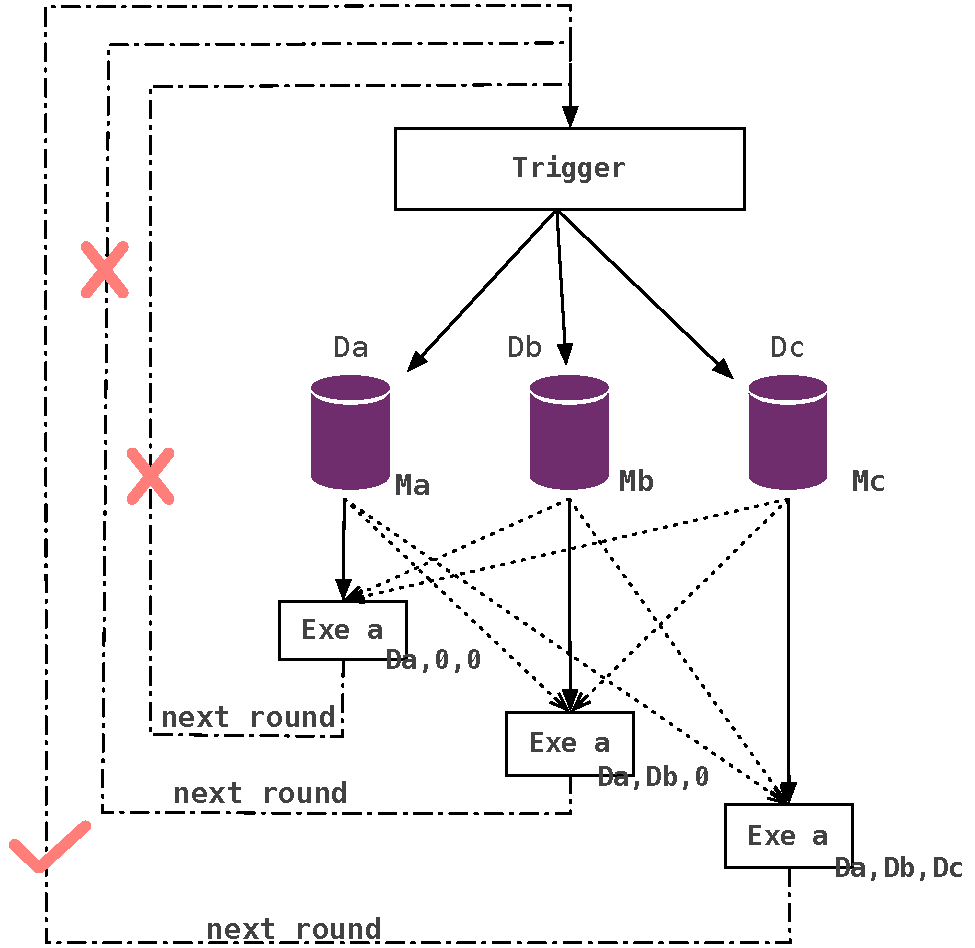
\includegraphics[width=5in]{../figures/sync.pdf}
\caption{最终同步的基本概念}
\label{fig:sync}
\end{figure*}

最终同步模型中,程序的执行不需要等待所有的子任务都完成,程序可以提前向下执行,但是在足够的时间窗口后,最终还是会得到同步执行相同的结果。图\ref{fig:sync}列举了在三台服务器($Ma, Mb, Mc$)上执行的三个触发器动作需要进行聚合时的情况,聚合$Da, Db, Dc$三个值。服务器$Ma$上的触发器首先计算出$Da$,此时$Mb$和$Mc$都没有完成计算,此时计算不会等待,而是根据$Da, 0, 0$计算出结果(这里的0不是指值为零,而是数据版本号为0,可参考下面的描述);随后$Mb$和$Mc$先后完成计算,产生了$Da, Db, 0$和$Da, Db, Dc$两个值。最后触发的$Mc$产生的值会覆盖掉之前的部分值,作为最终同步的结果出现。

Domino中最终同步模型基于HBase的多版本表实现,它可以用于同步两个不同的触发器,也可以用于上一节我们描述的聚合模式。比如,当用户需要聚合操作,并且需要在聚合操作处进行同步的时候,只要伴随需要聚合的触发器再提交一个聚合触发器即可。系统会自动创建一个仅本应用可以访问的隐式表,该表存储的所有数据都是带有版本信息的。表中任一个cell上数据的版本信息等于将该数据写入表的触发器动作的执行序列id,而触发器动作的执行序列id则是从0开始,每次执行自动加1的。聚合触发器的动作(Action)则根据表上的数据更新操作来执行:每次数据更新都会触发动作执行用户定义的聚合操作,那么这个动作的执行序列id就是更新后的数据的版本号。执行聚合操作需要读入表的数据,Domino模型确保该函数只能读到小于或等于当前执行序列id的数据,最终产生的结果的版本id也是当前动作的执行序列id加1。

\begin{figure*}[h!]
\centering
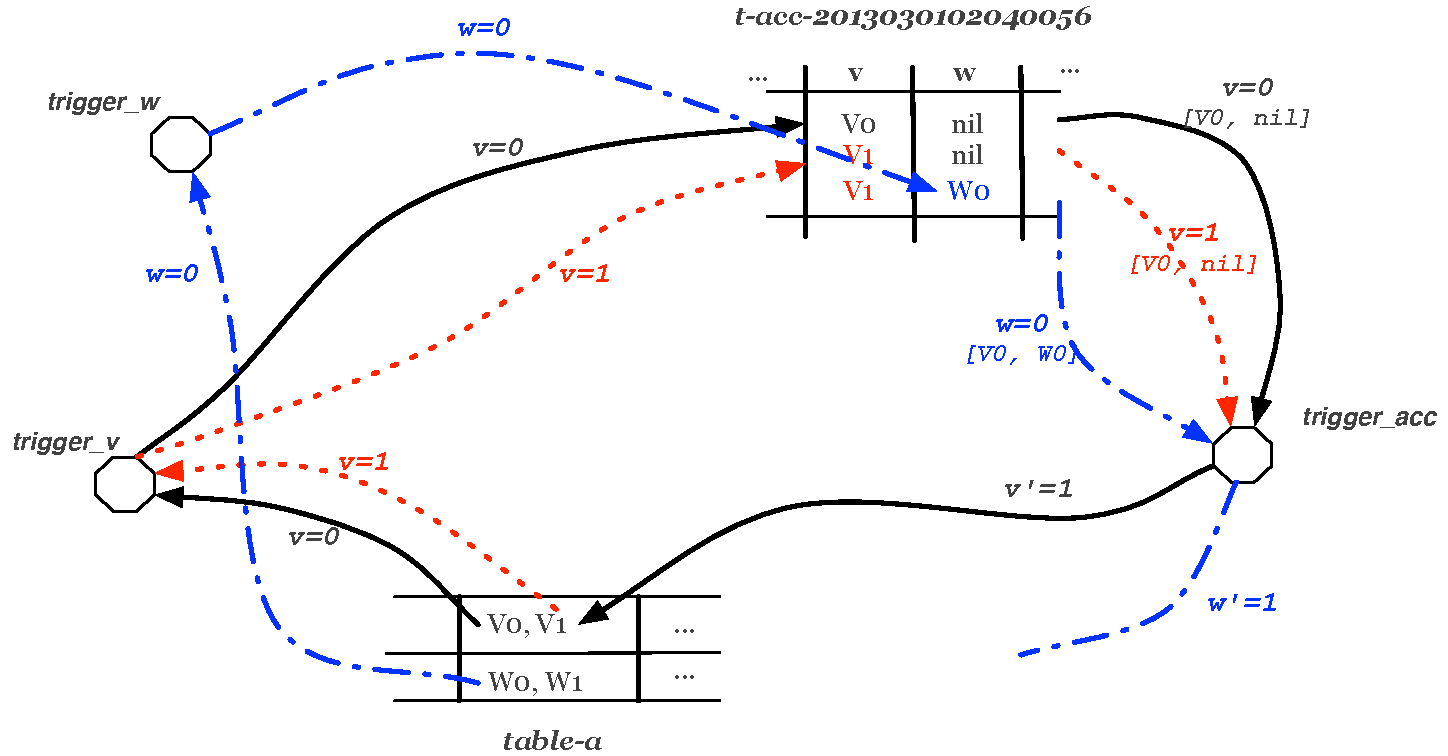
\includegraphics[width=5.5in]{../figures/multiv.pdf}
\caption{Domino中最终同步模型下多版本执行的流程图}
\label{fig:multiv}
\end{figure*}


图\ref{fig:multiv}展示了这样一个最终同步模型下多版本执行的流程。我们使用了两个触发器:$trigger_{[w|k]}$和$trigger_{acc}$来做示例。其中$triger_{[w|k]}$由表$table_a$触发,而$trigger_{acc}$用来帮助同步所有$trigger_{[w|k]}$实例产生的中间结果。表名字为t-acc-2013030102040056,由Domino系统自动创建,且仅在$trigger_{acc}$中可以访问。由图中可以看出$trigger_w$比$trigger_v$慢一些,当$v$已经运行到执行序列为1的时候,$w$刚刚开始它第0轮运行。那么在整个执行过程中,两个中间结果会被聚合触发器的动作函数根据输入$[v_0, nil], [v_1, nil]$计算出来并且写入到HBase的表中。这些结果未必正确,但是它能够作为中间结果被访问和使用。如果我们的算法中这些部分结果是有意义的,那么这些部分结果就能够被最早的加以利用,而不是所有的节点都等待最慢节点的执行。当然,随着$w$的执行,其最终也会将结果写入到表中,聚合函数根据版本顺序,取到的输入正好是所有同版本的数据,从而得到正确的结果。

最终同步相比较严格同步来说,不会发生停止等待的情况,不需要分布式锁的参与。特别对于那些中间结果有意义的算法具有非常好的效果,且其本身也可以保证最终结果与同步模型结果完全相同。因此在实际应用中有很多优势。不过其问题也非常明显,其中最大的就是资源浪费问题,如果大量的中间结果是无意义的,那么浪费计算资源去计算它们就没有意义。因此对于这类算法,还是应当采用严格同步的模型。

由于在最终同步的实现中,所有的序列id都是本地维护的,这样就存在一种可能性:具有相同执行序列的动作函数都试图向同一个位置发起写操作。在这种情况下,我们需要对这些写操作指定一个顺序来保证结果的正确性。在Domino中,我们定义一个触发器的某个动作函数的写序向量如下:
\begin{equation}
V^{T} = (V_{tc_{fired}}: V_{tc_1} : V_{tc_2}: ... V_{tc_i})
\end{equation}
其中等式右边的$V_{tc_{fired}}$代表触发该触发器动作执行的数据版本号,而$V_{tc_i}$则代表了触发器动作执行时访问的数据的版本号。当两个具有相同的触发器动作执行序列号的动作($i$和$j$)试图向同一个位置写入数据的时候,系统将比较他们的写序向量:首先比较$V_{tc_{fired}}^i$ 和 $V_{tc_{fired}}^j$,较大的动作写入;若相等,那么从前向后依次比较$V_{tc_i}$,同样是较大的动作写入。

通过这种方式设计的写顺序,通过简单的分析就可以知道:任何时候,一个全部到达同步点的写入带来的触发器动作一定比所有未完全到达同步点的触发器动作的写序向量大,这样就保证了最终同步的结果不会被覆盖。

\section{设计和实现}
\label{section:design}
本节中我们将介绍Domino运行时系统的实现以及其主要挑战的解决方法。我们将Domino系统设计成为使用Java实现的基于HBase的计算模型,并且和HBase以一种插件的方式一起运行,然而事实上Domino的实现并不限制与HBase,它可以与任何的分布式存储系统一起工作,只要存储系统提供持久性支持并且允许存储多版本的数据。我们现在正在将Domino移植到Sedna系统中。


\begin{figure}[h!]
\centering
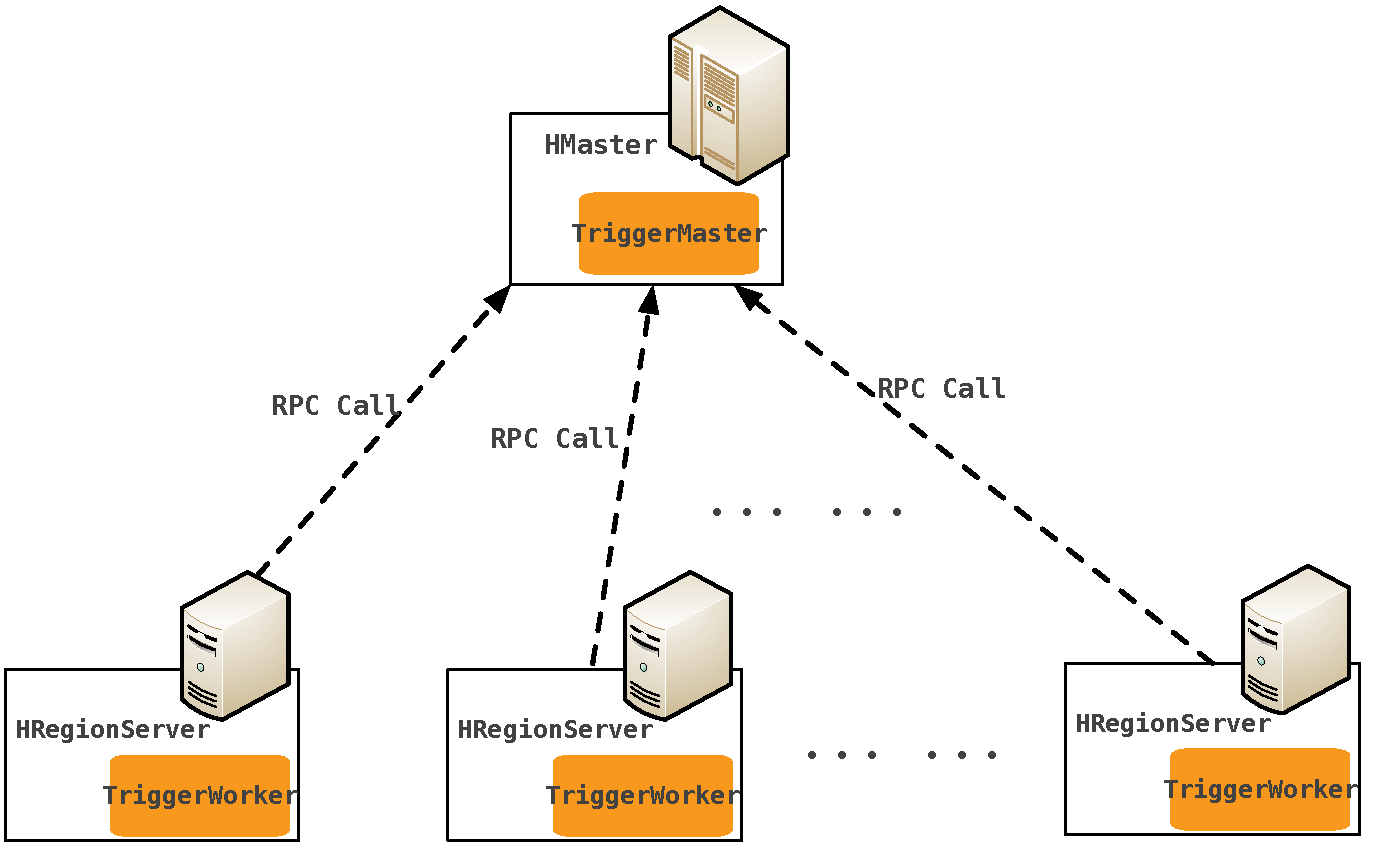
\includegraphics[width=5in]{arch1.pdf}
\caption{运行在HBase集群上的Domino集群的架构图}
\label{fig:arch1}
\end{figure}

\begin{figure}[h!]
\centering
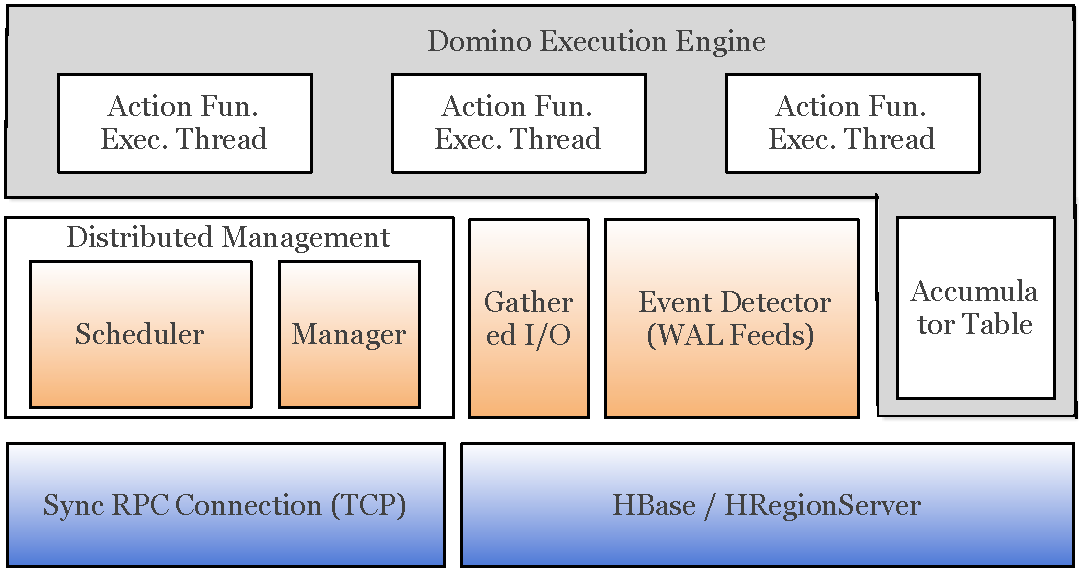
\includegraphics[width=5in]{../figures/arch.pdf}
\caption{Domino运行时系统的模块图,每一个模块都依赖于其下面模块提供的服务}
\label{fig:arch}
\end{figure}

图\ref{fig:arch1}和\ref{fig:arch}分别展示了Domino的系统架构以及不同逻辑模块之间的逻辑架构。Domino本身是基于HBase实现的,因此在实际运行中其节点之间的架构和HBase一致,都是由Master节点和Slave节点组成。HBase中的Master节点称为$HMaster$,slave节点也就是实际的Region存储的节点被称为$HRegionServer$;于此对应的是Domino的节点,Domino的Master节点$TriggerMaster$与HBase的$HMaster$运行在同一个物理节点上,而任务执行节点$TriggerWorker$运行在$HRegionServer$的节点上。所有的节点都运行着图\ref{fig:arch}中的各个组件,唯一的区别是$TriggerMaster$会运行其中的分布式管理(distribted management)部分,而$TriggerWorker$则不会运行这部分。不同的$TriggerWorker$之间通过同步的RCP远程调用来互相通信,而所有的$TriggerWorker$也需要和$TriggerMaster$保持一个心跳连接以汇报所有触发器的执行状态。需要注意的是,Domino的$HMaster$不是由用户手工指定的,而是在Domino启动的时候首次将自己注册成为$TriggerMaster$的节点充当。因此在Domino中不存在单点故障或者单点性能瓶颈。

\subsection{执行流程}
用户想Domino系统提交触发器采用MapReduce任务提交类似的方式:首先将需要执行的触发器相关代码打包成jar包,然后通过domino命令行程序提交到系统中去。下面的代码块展示了如何将上文中实现的分布式触发器提交给Domino的命令。其中WBCrawler为一个包含了main入口的主类,其负责提交另外WBContentTrigger和WBUserTrigger。
\begin{lstlisting}[language=bash]
	bin/domino trigger WBCrawler.jar wbcrawler.WBCrawler
\end{lstlisting}

用户向Domino提交触发器是通过新建并初始化一个Trigger对象,之后调用其submit方法实现的。下面的代码块展示了分布式爬虫实现中一个触发器(WBUserTrigger)的提交代码。用户需要新建一个Trigger对象,这个对象中必须设置触发器的名字,指定所监测的表、列族信息。如果这个触发器的检测对象具体到列族中的某个列,那么还需要调用配套的设置函数来设置,最后最重要的是需要设置该触发器触发时执行的类。这个类中应当包括用户实现的条件函数和动作函数。

\begin{lstlisting}[language=java]
Trigger tg2 = new Trigger("WBUserTrigger", "WBUser", "Activity");
tg2.setTriggerOnColumn("recently");
tg2.setActionClassName("wbcrawler.WBUserTrigger");
tg2.submit();
\end{lstlisting}

调用Trigger对象的submit函数后,Domino会首先从$TriggerMaster$处获得一个全局唯一的触发器id,之后将用户提交的jar包提交到HDFS存储系统由该触发器id组成的目录中。之后所有的$TriggerWorker$都将HDFS的该位置下载并加载需要的类。Domino会首先向$TriggerMaster$提交触发器。提交成功之后,会询问HBase的.META.表来获取本触发器所监测的表所在的$RegionServer$的位置。之后会依次向这些$RegionServer$提交触发器请求。只有所有的触发器请求都成功之后,提交才会返回。如果其中出错,Domino会负责回滚之前的操作,并且返回用户提交失败的信息。

触发器提交成功之后就已经开始在$RegionServer$处开始运行。此后,Domino在每一台服务器上都运行着事件感知组件(\ref{subsection:feed})负责监控数据更改,当遇到对象的数据修改的时候,用户提交的触发器代码就会被加载执行。触发器会因为停止条件(stop condition)而停止,也可以由用户提交命令显示的停止。在Domino中,用户程序可以使用Trigger对象的stop()方法来卸载一个触发器,也可以使用shell命令来完成:
\begin{lstlisting}[language=bash]
	bin/domino stop_trigger trigger-id
\end{lstlisting}
命令提交后,Domino会首先根据用户提交的‘trigger-id’来查找对应的trigger实例。如果存在,就会先卸载运行在$TriggerWorker$上的实例,所有实例卸载完成之后再卸载$TriggerMaster$上的实例,完成后返回。

\subsection{事件感知组件(Event Detector)}
\label{subsection:feed}
Domino的事件感知组件包括两部分。第一部分(WAL Feeds)作为主要的事件感知源用于在正常情况下对数据修改进行快速的感知;而另外一部分(Sequential Scan)则作为持久化事件的组件存在,当系统中出现错误的时候,该部分则保证所有未处理的事件都不会丢失。

\subsubsection{WAL Feeds}

HBase是一个保证了数据持久存储的分布式存储系统,它不会因为少量节点的故障而丢失数据。这是因为其会将所有的数据都存储在磁盘中,而磁盘则利用HDFS提供的多备份来保证数据的安全性。然而由于磁盘的响应时间过慢,为了提高IO性能,HBase会将所有的数据暂时存储在内存中,同时持久化在HDFS的WAL(write-ahead-log)中。为了保证数据不会因为在写操作的过程中节点突然崩溃而丢失,HBase会先将数据写入到WAL中,并且在写入成功后才开始将数据写入到内存中。写入到WAL中的数据是按照其在内存中的结构组织来写,而是将每一条数据整理成包括:行关键字、列族、列、值、时间戳、类型的日志,以顺序的方式写入WAL文件中,以提高磁盘I/O性能。

Domino的事件感知组件利用了HBase存储数据的特点,在每一个$TriggerWorker$中,Domino的事件感知组件都会将自己注册到HBase写入WAL文件的关键路径中,完全异步地对当前写入的日志数据进行判断,判断是否属于某个已注册的触发器所监测的范围。

\begin{figure}[]
\centering
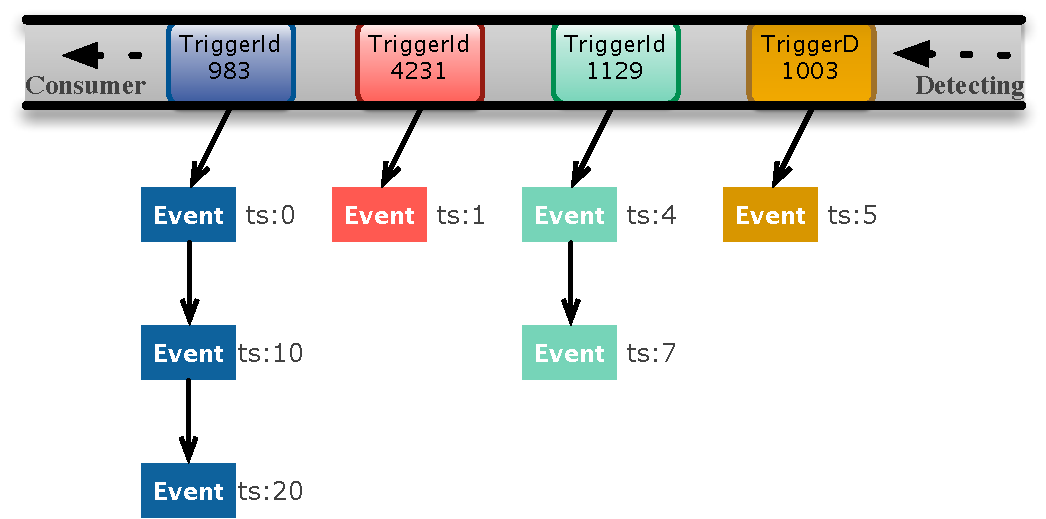
\includegraphics[width=5in]{../figures/queue.pdf}
\caption{Domino事件队列。如果两个事件属于同一个触发器,它们会整合被放入到队列中的同一个位置。队列中的顺序基于时间戳。消费者每次队列中取出属于同一个触发器的所有事件以减少频繁的进行线程切换带来的性能损失。}
\label{figs:queue}
\end{figure}

一旦事件感知组件探测到了一个对WAL文件的修改,并且该修改正好属于某一个已经注册的触发器的监测范围,它将封装一个包括了更新后的值以及更新前的值的事件(HTriggerEvent)并且将封装好的事件对象放入到事件队列中(如图\ref{figs:queue})所示。队列上有一个消费者不断的从队列中取出最新的事件来处理。最终,触发的事件会被发送到用户所写的条件函数和动作函数来处理。为了进一步提高效率,我们在每一个$TriggerWorker$中预先开辟了一个线程池,且为每一个触发器启动了一个线程,并且空置等待着事件到来执行。在实际的实现中,我们扩展了Java的同步线程库,使得所有的线程都变得可管理。具体表现在所有的子线程都有自动的异常处理、执行状态记录、重启等功能。

\subsubsection{顺序扫描}
WAL Feeds 组件对事件相应时间较低,适合作为主要的事件感知组件在Domino中运行。然而由于它的核心组件——事件队列是一直存在与单节点的内存中的,如果节点出现故障就无法恢复。这对于一个会长时间运行的分布式运行时系统来说是不可以接受的。为了在保证事件感知效率的前提下提高系统容错的能力,我们引入了Sequential Scan的策略来为Domino提供错误情况下的事件探测工作。

首先,由于Domino允许最小的监测单元是列,而HBase本身是将表按照列族分为独立的单元来管理的,因此同一行且同一个列族的数据一定在同一台服务器上存储着。我们修改HBase代码,为每一个列族默认的增加一列(\_events\_),每次HBase在向某一列族中的某一列写入数据的时候,系统会同时在\_events\_列中存储此次写入的本地唯一id,这个本地唯一id也会被存储到$HTriggerEvent$对象中,传给动作函数。用这样的方式,在WAL文件中,就会生成连续的两条写入日志:数据列写入和\_events\_列写入。另外一方面,当用户提交的触发器动作函数执行完毕的时候,Domino会自动将id从\_events\_列中删除。

如果Domino在运行过程中,某个节点崩溃,那么我们在WAL Feeds中所构造的事
件队列全部丢失,此时触发器会在另外一个节点上重新启动,而所有的崩溃节点
的数据也会在另外一个节点上由WAL文件进行恢复。在恢复的过程中,我们可以首先获得每一行数据,每一个列族的\_event\_列最新数据。上面记录了在事件队列中丢失了的所有的写入时的id。对每一个id,从后向前,逆着事件顺序搜索,当发现带有该id的WAL日志的时候,其前面那一条日志中存储的数据就是导致事件发生的,更新的数据的值。Domino会强制重新产生这个事件,进而继续之前未能执行的触发器动作。


\subsection{延迟写组件(Gathered I/O)}
\label{section:io}
Domino为用户提供了面向数据的编程模型,它允许用户在自己编写的函数中自由
的访问数据。但是这种模型也会带来很多问题。首当其冲的就是性能问题,因为
访问非本地数据是非常耗时的,而用户写的函数中可能多次调用这样的写操作从
而使得情况更加糟糕。另外一个问题就是数据的一致性问题,前面在介绍最终同
步的时候,我们介绍了如何解决同一个触发器不同的动作之间写冲突时一致性的
方案,而这里需要考虑的是不同触发器的写冲突。首先,对于单个写操作,在
Domino中,我们始终保证后写成功。在这个前提下,我们面临一个更复杂的情况:
由于我们允许用户自由的读写数据,那么有可能发生不同的触发器动作会进行交
错的写操作。比如触发器A写入$loc_1$,且成功,之后开始写$loc_2$;而触发
器B先写入$loc_2$成功后写入$loc_1$,这样最后结果是$loc_1$被A写入,
$loc_2$被B写入,任何一个触发器内部都无法得到一个一致的状态。

为了解决这些问题,在Domino中,我们提供了一个延迟写组件(WritePrepared)
帮助提高写效率,同时帮助在一个触发器内部维持一个一致的数据状态。
WritePrepared封装所有在触发器动作函数中发起的对HBase表格的写操作,并且
通过在一次动作函数执行完毕的时候调用flush方法来一次性的将WritePrepared
中缓存的数据真正写入到HBase的表格中。

WritePrepared中的缓存数据写入HBase表时是有序的,顺序是由调用flush操作
的时候从ZooKeeper获得的全局序列id($G_{id}$)决定的。当两个具有不同全局
id的写操作从Domino的触发器中发出的时候,如果两者并没有冲突(即没有写入
同一个位置),那么HBase并不会感受到有什么不同;然而如果两者产生冲突,那
么具有较大的全局序列id的写操作会被挂起直到前一个写操作完成。在挂起期间,
所有之前部分写成功的数据都会被冲突的那个、具有较小的全局序列id的写操作
覆盖。WritePrepared的flush顺序并不意味着我们将所有的分布式写操作都强制
排序了。强制对所有写操作排序会极大的降低写性能,我们只是通过版本控制保
证具有较低的全局id的flush操作开始后,它就不会被别的触发器抢占。

使用WritePrepared和flush操作,我们可以为触发器中的动作函数提供较高的
I/O效率,并且保证所有的写操作不会互相交错。

\subsection{容错和恢复组件}
容错能力是云计算平台下的计算模型面临的的最大的挑战。很多流式计算模型,
像Storm和S4这样的系统虽然具有较好的性能,但是其在容错和恢复上的短板同
样极大的限制了其应用。然而,Domino由于采用了基于触发器的模型,所有的中
间数据都可以保存在持久存储的分布式存储环境中使得我们能够有机会提供较好的容错能力以及错误恢复能力。

首先,Domino的各个组件通过HBase提供的容错能力作为其静态容错的基础:所
有提交的触发器信息都存储在HBase中,所有中间数据都被保存在HBase表中,触
发器的执行状态也通过序列id区别保存,聚合模式中自动创建的分布式表
($t_{acc}$)也持久存储在HBase中。这些信息都不会因为节点的意外崩溃而丢失。

除了静态容错外,由于触发器在Domino系统中时刻处于运行的状态,我们希望能
够对执行中的状态实现容错和恢复。比如正在执行的触发器所在的节点崩溃,或
者触发器本身线程崩溃,我们希望能够尽快的在备份节点上继续之前正在进行的
计算。

Domino节点中比较极端的情况是物理节点崩溃,这也意味着其上面运行的HBase
服务也离线。那么节点崩溃之后的所有更新操作都会被重定向到自动选出的备份
节点,并且在备份节点上会开始根据WAL中的数据重建内存数据结构。在备份节点恢复数据的同时,Domino的触发器会随之重新在备份节点上初始化并且开始运
行。这意味着,所有在节点崩溃之后新的数据写入操作都会如同没有发生错误一
样在新的节点上被触发器监测并且处理。

对于那些崩溃发生时正在执行的动作函数来说,所有能影响到HBase的输出都被缓存在WritePrepared中。若崩溃时尚未执行到flush,那么该动作函数的本次执行未完成,Domino在备份节点上重新运行该动作函数即可(只读入对应该执行序列id的输入数据);若崩溃时已经开始执行flush,那么这次动作函数的执行其实已经完成,只剩下最后的IO操作。为了能够保证完成所有的缓存在WritePrepared中的IO操作,在Domino中,除了前面所讲每一个的WritePrepared都在ZooKeeper中申请全局唯一序列号($G_{id}$)
外,我们还为每一个WritePrepared实例都在ZooKeeper上映射了一个临时节点,
其中存放序列化好的HBase写入操作序列以及当前执行完的操作id,这样保证一
旦flush开始就能够完整结束。

在Domino中用户提交的触发器代码并不是像MapReduce中那样运行在独立的JVM中,而是运行在$TriggerWorker$所在的JVM中。这样做主要是由于用户提交的触发器是常驻系统执行的,其执行时间长,粒度较低,对响应时间要求较高。如果每次提交触发器都要在相关的$TriggerWorker$上生成新的JVM运行的话,那一台服务器所能处理的触发器数目就极为有限。

但是将用户提交的函数放在Domino所在的JVM执行需要面临不可控代码带来的错误和异常。在Domino中我们在每一个$TriggerWorker$中实现了一个$LocalThreadManager$类,它负责在初始化的时候预先开辟一个线程池供用户提交的触发器使用;除此之外,该类会记录所有的触发器和线程的对应关系;最重要的是其会尝试catch所有来自用户提交的函数产生的错误和异常(通过捕获Java的Throwable对象实现)。这样当$LocalThreadManager$发现某一个线程出现未处理的错误或者异常的时候,它会按照系统的要求进行处理使其不会影响到$TriggerWorker$的正常执行。

\subsection{优化}
Domino的设计和实现为面向需要快速给出答案的迭代和递增处理应用,尽管通过基于触发器的编程模型以及HBase的高随机读写的特点,我们已经提供了非常有竞争力的任务执行速度,但是我们依然希望能够进一步的提升系统执行速度,降低资源占有率。本章将主要介绍在Domino系统的两个优化。

\subsubsection{内存加速}
考虑Domino中的一个迭代应用,在触发器多次执行的过程中,我们需要将所有的中间结果写入到HBase的表中。这样做最主要的原因是我们需要这些针对HBase中表内容的修改才能触发下一轮的触发器执行,当然把这些中间结果写入到HBase的表中也能够提高系统日后容错恢复的能力。但实际情况是,在系统没有发生错误的情况下,我们对这些中间结果并不关心,我们只是希望尽快的得到最后的正确结果。因此,为了提升Domino中应用程序执行的速度,不将系统资源浪费在存储不关心的中间结果上,我们引入了内存加速的方案。

在Domino中,编程人员可以通过改变WritePrepared对象的参数来使得所有写的写操作不写入到HBase表中,而是写入到Domino自动创建的分布式内存表中。该分布式内存表结构与HBase表相同,区别在于仅仅存储在分布式的内存中,写操作不需要持久化到WAL中,因此其性能远优于HBase。Domino应用程序在迭代执行过程中产生的所有的中间结果可以通过这种方式存储在WritePrepared所创建的分布式内存表中,而后续的触发器则可以通过监测这个分布式内存表来产生下一步的事件,并且加以处理。当触发器结束执行的时候,该触发器的WritePrepared对象所关联的分布式内存表将被转化成为真正的HBase表持久化储起来。

使用内存加速能够极大的提高Domino下应用程序的执行速度,它特别适合那些需要较快计算出结果的迭代例程。不过,我们在上面的描述中也同时指出了,内存中的数据都是不安全的,任何一个错误都会导致整个计算重新开始,因此对于那些需要长时间运行的应用程序,使用这种策略反而可能会延长计算时间。面对这种应用,我们可以将其分解成为若干步互相依赖的短的任务,并且对每一个短任务使用内存加速,这样就能够更快的计算出最终结果,并且对于计算中出现的错误也能够以较小的代价重新运行。

\subsubsection{负载均衡}
Domino系统中运行的所有应用都严格遵守了数据局部性的原则:所有的计算(触发器动作)一定在引起该触发器运行的节点上运行(尽管其执行过程中未必保证所有的读入数据都来自于本地节点)。这种特性对于提高计算性能是非常有利的,不过却容易出现负载不均衡的情况:比如HBase的某表的特定行范围被更新的频率明显高于其它表或者表的其他范围,而这个范围恰好又落在某一台服务器上,那么这个服务器就会面临更多的触发器执行,从而导致相应速度变慢。这种情况下,我们称表的这个部分为热区(hot spot)。在Domino中,我们考虑这种情况设计了简单的行负载均衡策略来对热区进行平均分配。

HBase中表格存储是按照行进行分割的,最开始一个空表存储在某一台服务器上。随着不断增加新的数据,表的行数也在不断增加,当表的行数增加到一定程度的时候,HBase会将这个表按照行进行分割,并且将两个子表存储在不同的服务器上。可以称这种做法为HBase的负载均衡。Domino的热区均衡就是基于同样的流程:HBase表的每一个区域(Region)的访问频度都被我们记录下来,当某一个表的大小超过的HBase允许的阈值,或者它的访问频度超过了Domino设置的访问频度上限,我们就将这个表进行分割,并且将产生的子表存储的不同的服务器上。表分割的同时,表上面设置的触发器也会跟着复制传输到另外一个节点。


\section{应用实例}
\label{section:apps}
之前我们已经详细介绍了Domino的编程模型以及其实现的细节,按照我们在本章开始之处指出的,我们希望Domino是一个通用的编程模型而不是像数据库中的触发器那样仅仅作为一个辅助工具出现。为了表明,现在我们设计的Domino具有这个能力,本节我们将介绍如何在Domino中实现几个比较经典的分布式应用: 搜索引擎中常用的PageRank算法;推荐系统中常用的协同过滤算法\cite{zhou2008large};数据挖掘中常用的$K$-means算法。这三个算法各具特色,在某种程度上能够体现出Domino的通用性。需要注意的是,在实现这它们的过程中,我们都只关注了最核心的算法部分的实现且并未针对性的进行优化。

\subsection{PageRank算法}
PageRank算法是最早由Google的创始人提出的计算互联网中页面重要程度的算法。它的输入是一个稀疏图,图中的每一个节点代表一个页面,每一个有向边代表了页面之间通过超链接产生的连接关系。它的思想很简单:那些被更多页面连接的页面更加重要。在实际计算中,我们将页面之间的连接关系抽象成一个网络图并且用一个矩阵$M$来表示,假设所有的页面的PageRank值最后组成一个向量$v$,那么PageRank的计算公式如下所示:

\begin{equation}
  \label{equation:pagerank}
v^{new}=\beta M v^{old} + (1 - \beta)e/n
\end{equation}

其中,$\beta$ 是一个选定的常熟,通常在0.8到0.9之间,$e$是一个全1向量,为公式合理性而加入的; $n$ 代表了所有页面的个数。PageRank算法会迭代的运行公式 \ref{equation:pagerank},直到 $v_{new}$ 和 $v_{old}$之间的差小于一个常数$\epsilon$。PageRank算法的实现也非常直白:首先为所有的页面设置一个初始的PageRank值$pr_i$,这样如果一个页面有$k_i$个向外的链接,那么每一个链接的权重就为$pr_i/n_i$。其次对每一个页面求所有指向自己的链接的权重和,比如有$ins$个指向自己的链接,那么当前页面新的$pr_i$的值就为$\sum_{k=0}^{ins}(pr_k/n_k)$。得到页面新的PageRank值之后,更新该页面所有向外链接的权重,继续执行下去。在得到页面新的PageRank值之后,是否马上更新所有链接权重,并且继续计所有别的页面的PageRank值体现了不同的实现策略。如果必须等待所有页面的新PageRank值计算完成之后才开始下一轮就成为同步实现,否则称为异步实现。实验和理论分析都证明,同步和异步的PageRank算法都能够得到正确的结果,并且异步算法速度优于同步算法,因此在本试验中,我们采用了异步实现。

在使用Domino模型编写PageRank之前,所有页面的信息首先应该存储在HBase中。表\ref{table:tm}展示了这样一个存储爬虫爬到的所有页面的信息表。表中每一行都是一个页面,每一个页面都有一个全局唯一的id;第一列pr属于列族prvalues,其中存储了当前页面的pagerank值;第二个列族存储了所有本页面中向外的链接指向的页面id,其中列的数目不确定,其余与PageRank计算无关的没有在表中列出来。

\begin{table}[ht]\small
\caption{HBase中\textit{webpages}表结构}
\label{table:tm}
\centering
\begin{tabular}{|c|c|c|c|}
\hline
\textit{WebPage} & \textit{prvalues:pr} & \textit{outlinks:[* any linkout]} & \textit{...}\\
\hline
$p_1$ & 0.5(default) & $p_{11}, p_{12}, p_{13}, ...$ & ...\\
\hline
$p_2$ & 0.5(default) & $p_{112}, p_{21}, p_{32}, ...$& ... \\
\hline
... & ... & ... , ... & ... \\
\hline
\end{tabular}
\end{table}

如表\ref{table:tm}所示,Domino的PageRank实现只需要在webpages表的'prvalues:pr'列上设置一个触发器,每当一个页面的PageRank值发生改变的时候,我们就根据列族outlinks中存储的链接信息更新每一个链接的权重。考虑到停止条件(stop condition),当任一个网页$wp_i$的新的pagerank值$rank^{'}_{wp_i}$和旧的pagerank值$rank_{wp_i}$的差小于$\epsilon$,我们就可以停止继续运行。因此停止条件为:
\begin{equation}
  Cond:true [r_{new} - r_{old} \leq  \epsilon]
\end{equation}

而根据当前页面的pagerank值更新所有的外链(指向其他页面的链接)权重的算法也非常简单,如算法\ref{alg:praction}所示:

\begin{algorithm}[]
  \caption{PageRankDist}
  \label{alg:praction}
  \begin{algorithmic}
    \REQUIRE Event object of current row ($e$)
    \STATE $n \leftarrow e.outedges$     //get out edges number
    \STATE $w \leftarrow e.rank/n $                //calculate out edge weight
    \FORALL{page $\in$ e.outedge[]}
    \STATE lazy-write(pr-acc, page, curr-page, w) //write into accumulator
    \ENDFOR
    \STATE Flush all written in lazy-write               //flush to available to other actions
  \end{algorithmic}
\end{algorithm}

在获得每一个链接的权重之后,我们需要对每一个页面计算所有指向它的链接权重的和。这是一个典型的聚合操作,因此我们使用了Domino提供的聚合模式来实现该方法。算法\ref{alg:praction}中使用lazy-write的时候,并不是将结果写入到HBase表中,而是写入到'pr-acc'这个聚合触发器中。这个聚合触发器作用于表\ref{table:acc}中。它监测着表的列族nodes,每当列族中数据发生改变的时候,聚合触发器就会通过求和得到当前页面的新的pagerank值,并且将新的pagerank值写入到表webpages的prvalues:pr中去。整个算法流程如\ref{alg:pracc}所示,具体的Java代码可见附录\ref{appendix:pagerank}。


\begin{table}[ht]\small
\caption{HBase中表\textit{pr-acc}的结构}
\label{table:acc}
\centering
\begin{tabular}{|c|c|c|c|}
\hline
\textit{WebPage} & \textit{nodes:[*any linkins]} & \textit{...}\\
\hline
$p_1$ & $p_{11}, p_{12}, p_{13}, ...$ & ... \\
\hline
$p_2$ & $p_{112}, p_{21}, p_{32}, ...$& ... \\
\hline
... & ... , ... & ... \\
\hline
\end{tabular}
\end{table}

\begin{algorithm}[ht]
  \caption{accumulator actions of \textit{pr-acc}}
  \label{alg:pracc}
  \begin{algorithmic}
    \REQUIRE distributed table $t_{acc}$. page-id as the row-key.
    \REQUIRE Each column represents the weights from one link-in edge.
    \FORALL{$weight_i \in$ $t_{acc}.columns$}
    \STATE $pr$ += $weight_i$
    \ENDFOR
    \STATE Flush $pr$ back to \textit{webpages} table
  \end{algorithmic}
\end{algorithm}

\subsection{协同过滤算法}
协同过滤算法是一种数据挖掘算法,主要用在推荐系统中。它能够根据已有的评分信息来预测尚未有评分信息的实体之间的关系。由于其有效性,大量应用在大型的互联网网站中。比如Netflix网上电影租赁系统会利用该算法根据用户已看过的电影以及评分信息来为用户推荐他们还未看过的电影。系统过滤算法也有很多种,本节我们将介绍一种称为\textbf{alternationg least squares (ALS)}的算法\cite{zhou2008large}在Domino上的实现,该算法曾应用在Netflix举办的第一届推荐系统大赛上,取得了非常好的效果。

ALS算法通过将一个拥有百万行列的稀疏矩阵表示成为两个较低维度的矩阵的乘积来预测那些原矩阵中缺失的数据。ALS的输入数据是稀疏矩阵$R$,其中包括了所有已知的评分信息(矩阵行代表了不同的用户、列代表不同的电影,每一个单元表示了某用户对某一部电影的评分信息)。ALS算法会迭代的计算出一个低维的矩阵分解,如公式\ref{equation:als}所示。

\begin{equation}
  \label{equation:als}
  R_{m,n} \thickapprox U_{m,d} \times M_{d,n}
\end{equation}

稀疏矩阵$R$是$m \times n$维的,其被分解成为两个低维矩阵$U$(m行d列)和$M$(d行n列)。具体的做法是先固定$M$,然后求出最好的$U$矩阵;之后固定$U$,求出最好的$M$。不断迭代,直到对已知数据的误差平方差小于一个小常数$\epsilon$。这里面$d$是可变的,值越大计算复杂度越高,但是结果对于输入数据的拟合度越高。在实际的应用中,通常我们设置一个比较合理的值来控制,比如20,来控制计算的时间。

不像PageRank算法,对于ALS算法本身的计算过程使用Domino的触发器模型来考虑并不是非常直观。不过使用触发器模型来实现该问题确有非常大的优势。相比较现有的ALS算法,Domino程序能够提供对不断增加、修改的用户评分信息提供实时的响应。在传统实现中,系统往往会选择周期性的重新执行ALS算法来处理过去一段时间增加的用户评价信息。这样,当输入数据集非常大,每次计算需要耗费大量资源的时候,就需要在推荐的实时性和资源使用成本之间做一个折中。使用Domino,由于对增量更新的处理需要较少的计算资源,使得实时的推荐成为可能。

首先,矩阵$R_{m,n}$被存储在HBase表(\textit{rating-table})中,这种大规模的稀疏表恰好是HBase存储的强项:每一个用户作为一行,其观看过的所有电影的评分信息存储在列'ratings:[* any movie]'中,即都存储在ratings列族中,而每一部电影都是列族中单独的一个列,如表\ref{table:rating}所示。Domino实现中,我们需要设置一个触发器监控rating-table的列族ratings,每当用户其中数据进行了修改(比如修改了$r_{i,j}$),我们就需要重新计算$U$的第i行和$M$的第j列的值,以使其能够拟合新的评分,并把新的$U$和$M$数据并且写入到聚合触发器(对应的表结构如表\ref{table:aslacc})中。与PageRank类似,聚合触发器将根据新的$U$和$M$的值来重新计算rating-table中的值,当新的值写入rating-table的时候又会触发下一轮对$U$和$M$的生成。不同的是,判断迭代是否应该中止的条件不是判断连续两次数据之差是否小于$\epsilon$,而是判断新的值和最初始值的差是否小于$\epsilon$。由于HBase支持多版本数据存储,这一点也很容易实现。

\begin{table}[ht]\small
\caption{HBase中的\textit{rating-table}表结构}
\label{table:rating}
\centering
\begin{tabular}{|c|c|c|c|}
\hline
\textit{Users} & \textit{ratings:[* any movie]} & \textit{...}\\
\hline
$U_1$ &  $p_{11}, p_{12}, p_{13}, ...$ & ...\\
\hline
$U_2$ &  $p_{112}, p_{21}, p_{32}, ...$& ... \\
\hline
... & ..., ... & ... \\
\hline
\end{tabular}
\end{table}


\begin{table}[]\small
\caption{ALS聚合表的结构}
\label{table:aslacc}
\centering
\begin{tabular}{|c|c|c|c|}
\hline
\textit{Entity} & \textit{vector:d-vector} & \textit{...}\\
\hline
$U_1$ &  $\left( v_1^{u1}, v_2^{u1}, ... v_d^{u1} \right)$ & ...\\
\hline
$M_1$ &  $\left( v_1^{m1}, v_2^{m1}, ... v_d^{m1} \right)$ & ... \\
\hline
... & ..., ... & ... \\
\hline
\end{tabular}
\end{table}

ALS算法实现中需要特别主意的是ALS算法对执行顺序的敏感性:ALS算法执行过程中,来自不同运算流程的更新如果没有序列化最终会影响$U$和$M$的收敛性。因此在ALS的Domino实现中需要使用严格同步模型来实现。

\subsection{$K$-means算法}
数据挖掘中,$K$-means也是一个被高频使用的聚类分析工具,它能够将未打标签的$n$个观测数据集根据彼此之间\textit{距离}的远近分割成为$k$个子类。$K$-means的正规定义如下:给定一个观察数据集$\left(x_1,
  x_2, ... x_n\right)$,其中每一个数据都是一个$d$维的实向量,$k$-means算法的目标就是将这$n$个数据分割成为$k$个集合($\left(k \leq n\right)$),S=($S_1, S_2, ...,
S_k$),使得单个集合内部所有点距离平均点的举例平方和最小:
\begin{equation}
  min\{\sum\limits_{i=1}^{k} \sum\limits_{x_j \in S_i}^{} ||X_j - \mu_i||^2\}
\end{equation}

$K$-means本身是NP问题,常见的解法是采用迭代逐步逼近的贪心算法。首先随即指定$k$个初始的聚类,其中每一个聚类的均值点是$m_1, ..., m_k$,接下来算法就迭代的进行下面两步:1)将每一个观测数据指派给它距离最近的集合;2)指派完所有的节点之后,计算新生成的集合的均值点。最终算法发现所有的观测数据的所属关系不再变化,就认为已收敛。

由上面的介绍我们可以知道$k$-mean算法是一个CPU密集型的计算任务。直观的来看,Domino提供的基于触发器的模型似乎和这种简单的计算密集型任务的关系不是很明确,实现起来也无从下手。

使用Domino模型编写应用程序的一个技巧:从收敛条件开始分析。我们注意到当$k$-mean发现所有节点的归属关系不再发生改变的时候就收敛结束了,那么我们第一个触发器一定要负责监控所有节点的归属关系。只有这样,我们才有可能正确的在收敛时停止运行。确定了触发器的检测表以及列族的信息后,我们就可以推断出HBase表的结构。比如在本例中,我们需要创建表\textit{cluster-table}来存储所有的$k$个聚类的中心点(存储在\textit{centroids:value}列中),并且所有属于该聚类的观测点(存储在\textit{clusterNodes}列中)。

\begin{enumerate}
\item 配置一个触发器(\textit{CentralTrigger})来监控表\textit{cluster-table}中的列\textit{centroids:value}。
\item 配置一个触发器(\textit{ClusterNodeTrigger})来监控同一个表的\textit{clusterNodes}列。
\end{enumerate}

程序刚开始执行的时候,首先产生随机的聚类中心点并且写入到表\textit{cluster-table}中,当然了此时这些聚类总还不包括任何的观测数据。该随机中心点的更新会导致\textit{CentralTrigger}中的动作执行,该动作会计算所有的存储在本地的观测单点和所有的聚类中心点的举例,得到最小的距离代表的聚类,并且将本观测点写入到聚类的\textit{clusterNodes}列族中。此时\textit{ClusterNodeTrigger}就会触发执行,它计算新的中心点,并且写入到列\textit{centroids:value}中。在$k$-means的实现中,不同的迭代之间需要严格的同步来保证最后结果的正确性,因此在这里我们使用了Domino提供的严格同步模型来实现该代码。

通过上面的分析可以看出来,在Domino模型下实现类似$k$-means的算法是有一些技巧的,它不像使用触发器模型写一个分布式网络爬虫那么直观,并且性能也很大程度上依赖着数据在不同节点上的存储时的平衡度。不过,我们依旧可以看出作为一个通用的编程模型,Domino依然能够为$k$-means这样的应用提供完善的支持。虽然直接计算$k$-means的效率和使用MapReduce模型相比优势并不明显但是如果考虑到不断变化的观察点求聚类的话,那么整个计算复杂度则依旧明显由于任何MapReduce的解决方案。


\section{实验分析}
\label{section:exp}

\subsection{实验环境设置}
我们通过对之前实现的多个应用程序(分布式爬虫、PageRank、协同过滤以及$k$-means算法)对Domino模型和运行时系统进行性能评测,对应比较版本为MapReduce实现。

大部分的实验都基于一个9个节点的本地集群实现,所有的节点都包含一个Xeon双核2.53GHz处理器以及6GB的内存,通过1Gb的以太网交换机连接。图\ref{fig:data}展示了每一个参与比较的应用程序的默认输入数据集大小以及最大的输入数据集。PageRank算法的默认输入来自于我们的分布式爬虫爬取到的1百万用户的页面信息。更大的输入数据集则来自于手工产生的10亿用户页面数据。协同过滤算法的输入数据来自于公开的电影评分数据集,所使用的最大数据集则使用随机生成的十亿条评分信息作为输入。

\begin{figure}[h!]
\centering
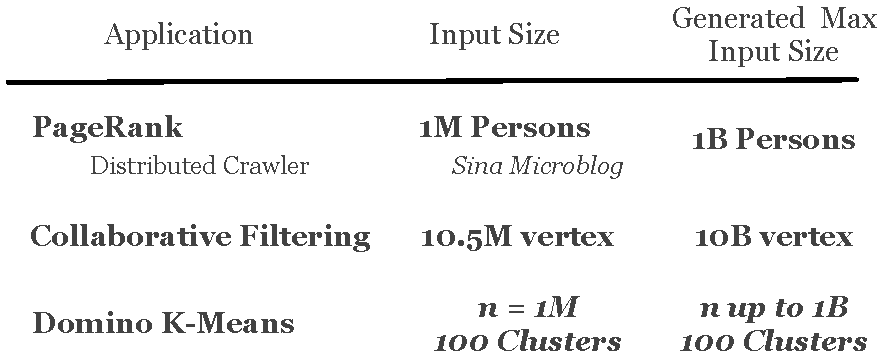
\includegraphics[width=4in]{data.pdf}
\caption{Domino相关测试输入数据大小}
\label{fig:data}
\end{figure}

\subsection{HBase性能比较}

按照我们之前的描述,Domino系统是基于对HBase的\textit{WAL}写动作进行监控实现的事件本地监测,并且通过向每一个\textit{RegionServer}添加本地周期扫描线程实现容错处理,除此之外,触发器的动作函数也是在HBase所运行的JVM中运行。因此这些操作一定会降低HBase本身的读写性能,本实验中我们将监测Domino实现本身对HBase系统性能的影响。本节所有实验都基于本地的9节点Domino集群实现。


\begin{figure}[h!]
  \centering
  \includegraphics[angle=270, width=4.5in]{gnuplot/cmphbase.eps}
  \caption{Domino和HBase写性能的对比图 1(Domino中无Trigger运行)}
  \label{cmphbase}
\end{figure}

\begin{figure}[h!]
  \centering
  \includegraphics[angle=270, width=4.5in]{gnuplot/cmphbaseouttrigger.eps}
  \caption{Domino和HBase写性能的对比图 2(Domino中Trigger高频率触发)}
  \label{cmphbase1}
\end{figure}

HBase的写性能测试中我们使用了\textit{PerformanceEvaluation}\cite{hbaseperformance}包,该包最早由HBase-399引入来测试HBase系统本身的读写性能。整个测试通过启动多个MapReduce任务完成,给定一个参数$n$,测试程序会在$n$台客户机上同时启动$10*n$个map任务,同时对HBase进行插入操作,每一个客户端将插入1百万行,每一行正好是1000字节。简单的计算可知,每一个map任务需要插入十万条。Reduce任务则比较简单,它会将所有的map中成功插入的条数做一个和,最后返回给用户。由于Reduce时间尽管没有对HBase进行写入,但依然会耗费大量的时间,因此在实际的比较中,我们将这一部分时间删去。为了更好的比较Domino和HBase的性能,我们根据整个MapReduce任务的执行时间计算出每一个map的平均执行时间,并且根据每一个map的平均写入条数来计算出单map的插入效率,通过乘以系统允许同时运行的map数目,最终得到整个HBase集群的写入速度。

图\ref{cmphbase}展示了当Domino中系统中没有触发器运行时与HBase的写性能的多次(共8次)试验的比较数据,此时所有的性能降低来自于我们的\textit{WAL Feeds}实现。我们发现Domino性能确有所降低,但是差别非常小(2\%)。图\ref{cmphbase1}则展示了当Domino系统中存在着频繁触发的触发器的时候系统的写性能与HBase的多次比较的结果。测试时我们对\textit{PreformanceEvaluation}所写的表设置了触发器,每次写入时,触发器都将执行。为了只检查触发本身的性能损失,触发器执行的动作非常简单,基本不占用CPU资源。从图中可以看出,即便在非常频繁的触发情况下,Domino和HBase相比性能下降依然在10\%以内。我们可以得出结论Domino本身实现带来的性能降低是非常小的。

\subsection{与MapReduce比较}

我们通过在Hadoop中实现了PageRank算法用以和Domino版本进行比较,而对于ALS算法和$k$-means算法我们采用了Mahout\cite{mahoutproject}中的实现。Mahout是一个基于Hadoop实现的饿开源大规模机器学习库,它包括了许多被高度优化的机器学习算法以及它们在Hadoop上基于MapReduce的实现。由于分布式爬虫没有任何可以基于MapReduce模型实现的必要,因此在本文中我们没有将其加入到比较中。

所有的实验都基于本地的9节点集群实现,所有的输入数据都是默认的输入数据,并且Domino使用了内存加速优化。在实验中,我们分别在3个节点和9个节点的集群上运行同样的应用以观察Domino应用和MapReduce应用的性能差别,以及进一步比较两种模型下应用的扩放性。从图\ref{spd}可以看出,在1百万个点的输入数据下,Domino的PageRank算法性能至少达到了基于Hadoop的PageRank实现的10倍以上的性能。而对于9个节点的集群来说,Domino下性能提升较Hadoop的提升也更大。

\begin{figure}[h!]
  \centering
  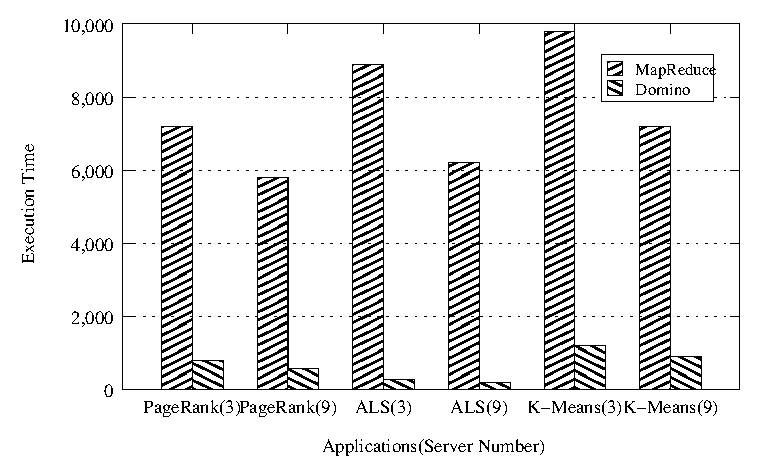
\includegraphics[width=5in]{gnuplot/cmpmapreduce.eps}
  \caption{PageRank、ALS、K-means算法的MapReduce实现和Domino实现的性能差别(3/9个节点)}
  \label{spd}
\end{figure}


从图\ref{spd}也可以看出ALS和$k$-means算法的性能提升同样非常明显,特别是ALS算法。这也很容易理解,由于Mahout中的ALS实现的每一个迭代包括了3个连续的MapReduce任务,这些MapReduce任务中所有的map函数并不进行计算,仅仅是为了将数据分发到不同的reduce函数中进行计算,这一切在Domino中都是不必须的,并且使用基于数据的模型是的Domino版本的ALS基本上不会进行多余的数据通讯。

\subsection{递增计算性能}

由于采用触发器模型,Domino模型最大的优势在于对递增计算的支持。PageRank的应用场景能够很好的体现这一点:通常情况下网络爬虫会不断的爬取新的网页交由PageRank进行排序。

\begin{figure}[h!]
  \centering
  \includegraphics[angle=270, width=5in]{gnuplot/increpr.eps}
  \caption{递增的PageRank在Domino和MapReduce下实现的性能对比}
  \label{incr}
\end{figure}

图\ref{incr}展示了Domino和MapReduce方案对于部分改变网页的计算性能对比。$y$轴表示了部分计算所花费的时间和全部都进行计算所花费时间的比率。基本的MapReduce语义中,无论几个页面发生了改变,为了得到正确的结果都需要对整个数据集运行一次完整的MapReduce程序。然而在Domino中,应用程序只需要对那些发生改变的页面以及与这些页面相关联的页面进行计算,因此Domino的递增计算性能远远好于MapReduce等系统:对于少量的输入数据集改变,可以立即得到新的结果。

\section{小结}
本章介绍了一个通用的基于触发器的编程模型及其运行时支持系统的设计和实现。通过引入聚合模式,我们在触发器这个纯异步模型的基础之上实现了同步语义;通过多版本数据管理,我们在Domino中引入了最终同步、严格同步模型,加上触发器本身的完全异步模型,为程序开发人员提供了针对应用可选的灵活模型。通过多种应用程序在Domino计算模型上的实现充分证明了该模型的有效性和通用性。除此之外,我们整合HBase存储系统实现了Domino运行时系统并且详细描述了各种优化策略,进一步提高其性能,应用的性能试验也证明了Domino运行时系统本身的高性能和高扩放性。Domino基于多版本数据管理为任务的容错和恢复设计了快速恢复的策略,能够有效的降低由于节点失效对整个应用执行速度的影响。

Domino并未对底层存储系统提出针对性的需求。带有容错和快速恢复功能的Domino仅要求底层存储系统能够提供数据持久化以及数据多版本存储的能力,因此Domino本身可以和多种存储系统整合起来以面向不同的应用场景。我们也正在进行这方面的工作,希望最终将存储系统和基于触发器编程模型模型紧密结合起来,作为云计算软件基础架构的核心组件存在。


  \chapter{结束语}

\section{研究工作总结}

本人博士期间工作和创新主要分为三部分:
\begin{enumerate}

\item 首先对现有的云计算基础软件架构的一个重要实现—Hadoop进行了系统的研究和应用测试,通过提出基于模糊逻辑的异构Hadoop集群的配置工具,简化了大规模异构的Hadoop集群的配置方式,提升了Hadoop集群上应用的执行速度。实验证明通过对Hadoop大规模集群的配置参数进行模糊推理和自动配置能够很大的提高系统性能。但是受限与MapReduce模型以及HDFS存储系统本身的特点,当面对基于海量数据的实时应用的时候,当前的云计算基础软件架构依然面临较大的挑战。应对这些挑战成为博士期间的核心工作。

\item 针对实时应用对分布式存储系统的数据访问速度的要求,我们设计实现了一个完全基于内存的分布式键值存储系统Sedna。通过使用内存作为主要存储介质,极大地提高了随机读写的响应速度和读写带宽。Sedna利用多备份实现了数据持久保存的能力,通过提出一种层次化的数据中心内存储系统的架构设计,Sedna结合一致性哈希和元数据集中管理的优点,提供了更好的扩放性性以及更灵活的负载均衡策略。我们还首次在Sedna中引入了基于触发器的文件读原语,通过监控数据的改变来帮助应用程序实时检测到数据的改变。

\item 针对新型的云计算平台上的复杂应用,我们提出了一个基于触发器的通用编程模型Domino,它能够更好的支持复杂的计算过程,比如典型的多次迭代和递增计算过程。除了将触发器模型引入到分布式处理中,并扩展成为一个通用的编程模型,Domino提出了聚合模式来解决多子任务数据同步的问题。Domino提出了多版本数据管理策略来实现最终同步的方法,进一步解决了在触发器模型下的数据同步问题,极大的扩宽了该模型的应用范围。我们还在Domino系统中首次完整的提出了对计算和数据进行容错以及恢复的算法。最后通过在不同应用上的使用实例也证明了Domino的可行性和效率。

\end{enumerate}


\section{对未来工作的展望}

通过之前的工作,我们建立了一个结合了Sedna和Domino的云计算环境的机会。通过扩展Sedna系统使其支持多版本数据的存储和管理,我们可以轻易的将现基于HBase的Domino编程模型移植到Sedna中。由于Sedna是一个完全基于内存的存储系统,通过和HBase的简单性能对比也可以看出来,其性能远远超过HBase,我们相信和基于Sedna的分布式存储系统的结合将进一步的提升Domino的计算速度。

其次Domino模型本身作为一种触发器模型更加适合递增计算,通过我们的之前的描述也容易注意到,对于某些复杂的大数据的数学计算其并不是非常适合,需要进行问题的转换后才能在Domino模型下实现。因此我们希望能够将Domino模型和现有的基于MapReduce的模型进行结合。对于存在大量数据时的首轮计算将采用MapReduce的方式计算,之后的改变则使用Domino模型进行计算。

另外,对于一个部署了Domino和Sedna的大规模集群来说,一样存在着资源管理优化配置的问题。我们相信基于模糊逻辑的Hadoop异构集群中提出的模糊逻辑思路对于提高集群的效率能够起到很好的指导作用。通过设计Domino和Sedna使其对动态改变配置更加友好,我们相信未来能够设计和实现一个运行时动态配置大规模集群的工具,用于进一步优化集群性能。




%\emph{Qingsong Liu}

%  参考文献测试:\citep{deng:01a}

  %参考文献测试:\citep{knuth86e}


%%%%%%%%%%%%%%%%%%%%%%%%%%%%%%
%% 附件部分
%%%%%%%%%%%%%%%%%%%%%%%%%%%%%%
\backmatter

  % 参考文献
  % 使用 BibTeX
  \bibliographystyle{ustcbib}%{GBT7714-2005NLang-UTF8}
  \bibliography{bib/tex}
  \nocite{*} % for every item
  % 不使用 BibTeX
  % %\renewcommand{\baselinestretch}{0.5}
\begin{thebibliography}{10}

\bibitem{deng:01a}
{邓建松,~彭冉冉,~陈长松邓建松,~彭冉冉,~陈长松邓建松,~彭冉冉,~陈长松邓建松,~彭冉冉,~陈长松邓建松,~彭冉冉,~陈长松邓建松,~彭冉冉,~陈长松邓建松,~彭冉冉,~陈长松邓建松,~彭冉冉,~陈长松邓建松,~彭冉冉,~陈长松邓建松,~彭冉冉,~陈长松邓建松,~彭冉冉,~陈长松}.
\newblock {\em \LaTeXe{}~科技排版指南}.
\newblock 科学出版社,~书号:~7-03-009239-2/TP.1516, 北京, 2001.

\bibitem{wang:00a}
王磊.
\newblock {\em \LaTeXe{}~插图指南}.
\newblock 2000.

\bibitem{zhang:03a}
张林波.
\newblock {\em 关于新版~CCT~的说明}.
\newblock 2003.

\bibitem{lshort-cn}
C\TeX{} 翻译小组.
\newblock {\em lshort~中文版~3.20}.
\newblock 2003.

\bibitem{knuth86e}
Donald~E. Knuth.
\newblock {\em Computer Modern Typefaces}, volume~E of {\em Computers and
  Typesetting}.
\newblock Addison-Wesley, Reading, Massachusetts, 1986.

\bibitem{knuth86d}
Donald~E. Knuth.
\newblock {\em {METAFONT}: The Program}, volume~D of {\em Computers and
  Typesetting}.
\newblock Addison-Wesley, Reading, Massachusetts, 1986.

\bibitem{knuth86c}
Donald~E. Knuth.
\newblock {\em The {METAFONT}book}, volume~C of {\em Computers and
  Typesetting}.
\newblock Addison-Wesley, Reading, Massachusetts, 1986.

\bibitem{knuth86b}
Donald~E. Knuth.
\newblock {\em {TeX}: The Program}, volume~B of {\em Computers and
  Typesetting}.
\newblock Addison-Wesley, Reading, Massachusetts, 1986.

\bibitem{knuth86a}
Donald~E. Knuth.
\newblock {\em The {TeX}book}, volume~A of {\em Computers and Typesetting}.
\newblock Addison-Wesley, Reading, Massachusetts, 1986.

\bibitem{lamport85a}
Leslie Lamport.
\newblock {\em {LaTeX} --- A Document Preparation System: User's Guide and
  Reference Manual}.
\newblock Addison-Wesley, Reading, Massachusetts, 2nd edition, 1985.

\end{thebibliography}


  % 附录
  \begin{appendix}
      \section{代码节选}
\subsection{\textbf{[分布式爬虫实例]}}
\label{code:wbcrawler}
\begin{lstlisting}[language=java]
/**
 * WBContentTrigger.java
 */
package wbcrawler;

//所有提交的触发器都需要实现HTriggerAction这个基类
public class WBContentTrigger extends HTriggerAction{

  //访问微博的凭证
  private final String accessToken = @access_token;
  private WritePrepared writer = null;

  //初始化读写其他表中数据所用的WritePrepared实例。
  public WBContentTrigger(){
    byte[] tableName = "WBRelation".getBytes();
    this.writer = new WritePrepared(tableName);
  }

  private ArrayList<String> getUsersByAPI(String msgId);

  //封装好的事件对象,其中包括了触发事件的表、行以及相关列族的内容数据。
  @Override
  public void action(HTriggerEvent hte) {
    byte[] msgId = hte.getRowKey();
    byte[] msgContent = hte.getNewValue();
    String msgContentStr = new String(msgContent);

    ArrayList<String> aus = this.getUsersByAPI(new String(msgId));
    for (String userId : aus){
      Put p = new Put(userId.getBytes());
      p.add("Activity".getBytes(), "recently".getBytes(),
      		  "true".getBytes());
      this.writer.append(p);
    }
    this.writer.flush();
  }
  //过滤器,用来判断这个事件是否应该使触发器执行。
  @Override
  public boolean filter(HTriggerEvent hte) {
    return true;
  }
}
\end{lstlisting}
\begin{lstlisting}[language=java]
/**
 * WBUserTrigger.java
 */
package wbcrawler;
public class WBUserTrigger extends HTriggerAction{
  ...
  ...
  @Override
  public void action(HTriggerEvent hte) {
	byte[] userId = hte.getRowKey();
	Timeline tl = new Timeline();
	tl.client.setToken(this.accessToken);
	StatusWapper status = tl.getUserTimelineByUid(new String(userId));
	for (Status s:status.getStatuses()){
		Put p = new Put(msgId);
		p.add("Content".getBytes(), "zh".getBytes(), s.getText().getBytes());
		writer.append(p);
	}
	this.writer.flush();
  }
  @Override
  public boolean filter(HTriggerEvent hte) {
    return true;
  }
}
\end{lstlisting}


\subsection{\textbf{[PageRank实现实例]}}
\label{appendix:pagerank}
\begin{lstlisting}[language=java]

public class PageRankDist extends HTriggerAction{

  private WritePrepared writer = null;
  private ReadPrepared reader = null;

  public PageRankDist(){
    boolean isAcc = true;
    writer = new WriterPrepared(`PageRankAcc`.getBytes(), isAcc);
    reader = new ReadPrepared(`wbpages`.getBytes[]);
  }

  @Override
  public void action(HTriggerEvent hte) {
    byte[] currentPageId = hte.getRowKey();
    float fvalue = Float.parseFloat(hte.getNewValue());

    Get g = new Get(currentPageId);
    g.addFamily("outlinks".getBytes());
    Result r = reader.get(g);

    outlinks = r.getFamilyMap("outlinks".getBytes());
    int n = outlinks.size();
    float weight = fvalue / n;

    for (byte[] link: outlinks.values()){
      Put p = new Put(link);
      p.add("nodes".getBytes(), currentPageId, weight);
      writer.append(p);
    }
    this.writer.flush();
  }

  @Override
  public boolean filter(HTriggerEvent hte) {
    byte[] nvalue = hte.getNewValue();
    byte[] oldValue = hte.getOldValue();
    float fnv = Float.parseFloat(new String(nvalue));
    float fov = Float.parseFloat(new String(oldValue));
    if (Math.abs((fnv - fov)) < 0.001){
      return false;
    }
    return true;
  }
}
\end{lstlisting}

\begin{lstlisting}[language=java]

public class PageRankAcc extends HTriggerAction{

  private WritePrepared writer = null;
  private ReadPrepared reader = null;

  public PageRankAcc(){
    writer = new WriterPrepared(`wbpages`.getBytes());
    reader = new AccModeReader();
  }

  @Override
  public void action(HTriggerEvent hte) {
    byte[] pageId = hte.getRowKey();
    Get g = new Get(pageId);
    g.addFamily("nodes".getBytes());
    Result r = this.reader.get(g);

    nodes  = r.getFamilyMap("nodes".getBytes());
    for (byte[] weight:nodes.values()){
      String sw = new String(weight);
      float fw = Float.parseFloat(sw);
      sum += fw;
    }
    Put p = new Put(pageId);
    p.add("prvalues".getBytes(), "pr".getBytes(), sum);
    this.writer.append(p);
    this.writer.flush();
  }
  @Override
  public boolean filter(HTriggerEvent hte) {
    return true;
  }
}

\end{lstlisting}

  \end{appendix}

  % 致谢
  
\begin{thanks}
博士毕业的前夕,回首在中国科学技术大学度过的将近十年的时光,深刻的感受到了作为科大学子的自豪和幸运。在这十年中,无数的老师和同学曾给与我无私的帮助,而我所从事的学习和研究工作,也都是在导师以及其他多位老师和同学们的指导帮助下进行的。没有他们就没有这篇论文,更没有即将博士毕业的我,在此完成论文之际,请允许我对他们表达真诚的感谢。

首先感谢导致周学海教授和实验室李曦副教授多年的指导和教诲,正是老师们给予的帮助带领我进入了分布式系统的研究领域。正是在周老师和李老师的教导下,我才能在硕士期间打下坚实的基础,能够在新的领域做出一点点工作。两位老师细致的治学态度以及宽广的胸怀让我收益终身。

感谢班主任钱海老师多年的关怀,钱老师作为我的指路人,更是博士期间的班主任,他认真负责的工作态度给我平添了无数的温暖。

感谢实验室杨峰、吴昊、毛熠路、张启元、高师姐、马宏星等师兄师姐的指点和照顾,特别感谢王超在我博士期间给予的帮助,与你的讨论使我收益良多;感谢贾刚勇、石亮等几位同班同学,感谢你们在过去的几年里对我的照顾和帮助;感谢孙明明、卢坤、陈涛、刘吉、王亚楠、唐长城等师弟师妹,我们在云计算实验室共同创造未来,一起经历过拼搏和成功的日子,感谢你们的陪伴和支持。需要感谢的人太多,没有办法一一举出您的名字,谢谢你们,陪伴我度过这美丽快乐的学生时代!

最后,感谢我父母一贯的鼓励和支持,你们是我追求学业的坚强后盾。感谢我的妻子廖奕。谢谢你过去5年里对我的支持,感谢你对我的理解!

\vskip 18pt

\begin{flushright}

~~~~代 栋~~~~

\today

\end{flushright}

\end{thanks}


  % 发表文章目录
  \chapter{在读期间发表的学术论文与取得的研究成果}

\noindent\textbf{已发表论文:}

\begin{tabularx}{0.97\linewidth}{>{\raggedleft\scshape}p{2cm}X}
Conference & \textbf{Dong Dai}, Xi Li, Junneng Zhang, Chao Wang,
Xuehai Zhou. Detecting Associations in Large Dataset on
MapReduce. \textit{International Symposium on Parallel and Distributed
  Processing with Applications(IWCDM), 2013}
\end{tabularx}

\begin{tabularx}{0.97\linewidth}{>{\raggedleft\scshape}p{2cm}X}
Conference & \textbf{Dong Dai}, Xi Li, Chao Wang, Mingming Sun, and
Xuehai Zhou. Sedna: A Memory Based Key-value Storage System for
Realtime Processing in Cloud. \textit{In the proceeding of IEEE
  Cluster'12 (IASDS 2012), 24-28, Sep, Beijing}
\end{tabularx}

\begin{tabularx}{0.97\linewidth}{>{\raggedleft\scshape}p{2cm}X}
Conference & Kun Lu, \textbf{Dong Dai}. HDFS+: Concurrent Write
Improvements for HDFS. \textit{The 12th IEEE/ACM International
  Symposium on Cluster, Cloud and Grid Computing, 2013}
\end{tabularx}

\begin{tabularx}{0.97\linewidth}{>{\raggedleft\scshape}p{2cm}X}
Conference & \textbf{Dong Dai}, Xi Li, Chao Wang, and Xuehai
Zhou. Cloud Based Short Read Mapping Service. \textit{In the
  proceeding of IEEE Cluster'12, 24-28, Sep, Beijing}
\end{tabularx}

\begin{tabularx}{0.97\linewidth}{>{\raggedleft\scshape}p{2cm}X}
Conference & Chao Wang, Xi Li, \textbf{Dong Dai}, Gangyong Jia, and
Xuehai Zhou. Phase detection for loop-based programs on multicore
architectures. \textit{In the proceeding of IEEE
  Cluster'12, 24-28, Sep, Beijing}
\end{tabularx}

\begin{tabularx}{0.97\linewidth}{>{\raggedleft\scshape}p{2cm}X}
Conference & Tao Chen, \textbf{Dong Dai} et al. MapReduce On Stream
Processing. \textit{International Conference on Intelligent Computing
  and Intelligent System, 2011}
\end{tabularx}

\begin{tabularx}{0.97\linewidth}{>{\raggedleft\scshape}p{2cm}X}
Conference & Gangyong Jia, Xi Li, Xuehai Zhou, \textbf{Dong
  Dai}. Architecture Support Predicting Method for CMP
Scheduling. \textit{In Proceeding of International Conference on
  Computer Research and Development(ICCRD), 2011}
\end{tabularx}

\begin{tabularx}{0.97\linewidth}{>{\raggedleft\scshape}p{2cm}X}
Journal & \textbf{Dong Dai}, Xuehai Zhou, Feng Yang, and Chao Wang. An
auto-configuration tool for heterogeneous hadoop cluster. \textit{In
  Journal of the Graduate School of the Chinese Academy of Sciences,
  2011}
\end{tabularx}

\vskip 1cm

\noindent\textbf{投稿中论文:}
\vskip 0.5cm

\begin{tabularx}{0.97\linewidth}{>{\raggedleft\scshape}p{2cm}X}
Conference  & \textbf{Dong Dai}, Xi Li, Kun Lu, Chao Wang, Xuehai
Zhou. Domino: A trigger-based Programming Framework in
Cloud. \textit{IEEE Super Computing, 2013}
\end{tabularx}

\vskip 1cm

\noindent\textbf{专利申请情况}
\vskip 0.5cm
\begin{tabularx}{0.97\linewidth}{>{\raggedleft\scshape}p{2cm}X}
\gray 专利 & \textbf{基于Hadoop集群的分布式监控系统及其监控方法,受理
  号:201110060308.1}

\end{tabularx}

\vskip 1cm

\noindent\textbf{参与的科研项目}
\vskip 0.5cm
\begin{tabularx}{0.97\linewidth}{>{\raggedleft\scshape}p{2cm}X}
\gray Period & \textbf{07/2011 --- 07/2012}\\
\gray Name & \textbf{RFP-07-999 Cisco Research Foundation}\\
\end{tabularx}

\begin{tabularx}{0.97\linewidth}{>{\raggedleft\scshape}p{2cm}X}
\gray Period & \textbf{03/2010 --- 08/2011}\\
\gray Name & \textbf{Jiangsu Research Project-BY128}\\
\end{tabularx}


\end{document}
